%%% Generic LaTeX document.
%%% Basically just a wrapper around the PRL template.
%%%
%%% AUTHOR: Salvatore Cardamone
%%%         University of Cambridge, 2017

\documentclass[preprint,nofootinbib]{revtex4-1}

%%%
%%% Package inclusions and package-specific settings 
%%%
\usepackage{amsmath}
\usepackage{amssymb}
\usepackage{amsthm}
\usepackage{xcolor}
\usepackage{braket}
\usepackage{float}
\usepackage{tabularx}
\usepackage{graphicx}
\graphicspath{images}
\usepackage{pgfplots}
\usepackage{rotating}
\usepackage{enumitem}
\usepackage[toc,page]{appendix}
\usepackage[mathscr]{euscript}
\usepackage{minted}
\usepackage{mdframed}

\usetikzlibrary{positioning,circuits.ee.IEC}

%%%
%%% Generic LaTeX settings and commands
%%%
% Get rid of the cursed indentation
\setlength{\parindent}{0cm}
\raggedbottom
\setlist[enumerate]{noitemsep, nolistsep}
\setlist[itemize]{noitemsep, nolistsep}

%%%
%%% Macros and shortcuts
%%%
\renewcommand{\vec}[1]{\mathbf{#1}}
\newcommand{\matr}[1]{\mathbf{#1}}
\newcommand{\im}{{i\mkern1mu}}
\newcommand{\ex}[1]{\mathrm{e}^{#1}}
\newcommand{\dx}[1]{\mathrm{d}#1\mkern1mu}
\newcommand{\dsqx}[1]{\mathrm{d}^2#1\mkern1mu}
\newcommand{\infsum}[1]{\sum_{#1=-\infty}^\infty}
\newcommand{\rect}[1]{\Pi\left(#1\right)}
\newcommand{\ddx}[1]{\frac{\mathrm{d}}{\mathrm{d#1}}}

\newcommand{\red}[1]{\color{red}{#1}}
\newcommand{\orn}[1]{\color{orange}{#1}}
\newcommand{\yel}[1]{\color{yellow}{#1}}
\newcommand{\grn}[1]{\color{green}{#1}}
\newcommand{\blu}[1]{\color{blue}{#1}}
\newcommand{\st}{^\mathrm{st}\mkern1mu}
\renewcommand{\th}{^\mathrm{th}\mkern1mu}
\newcommand\fnorm[1]{\left\lVert#1\right\rVert}
\DeclareMathOperator{\sinc}{sinc}
\DeclareMathOperator*{\argmin}{arg\,min}

% Get rid of stupid revtex numbering
\def\thesection{\arabic{section}}
\def\thesubsection{\arabic{section}.\arabic{subsection}}
\def\thesubsubsection{\arabic{section}.\arabic{subsection}.\arabic{subsubsection}}
\def\theparagraph{\arabic{section}.\arabic{subsection}.\arabic{subsubsection}.\arabic{paragraph}}

\theoremstyle{definition}
\newtheorem{exmp}{Example}[section]
\newtheorem{iden}{Identity}[section]

%%%
%%% Document start
%%%
\begin{document}

%%%
%%% Document preamble
%%%
\title{DSP Lecture Notes}
\author{S. Cardamone}
\date{\today}

\begin{titlepage}
\maketitle
\tableofcontents
\end{titlepage}

%%%
%%% Actual document files
%%%
\section{Lecture 1: Introduction}

\subsection{Some Common Operations on Signals}
%
For the sake of introducing some basic definitions with which we can gain some
physical intuition, we'll define a \textbf{signal} as a stream of information
which originates from a sensor (and isn't necessarily indexed by time), and a
\textbf{system} as an entity which processes signals and produces other signals.
%
\begin{figure}[!htb]
  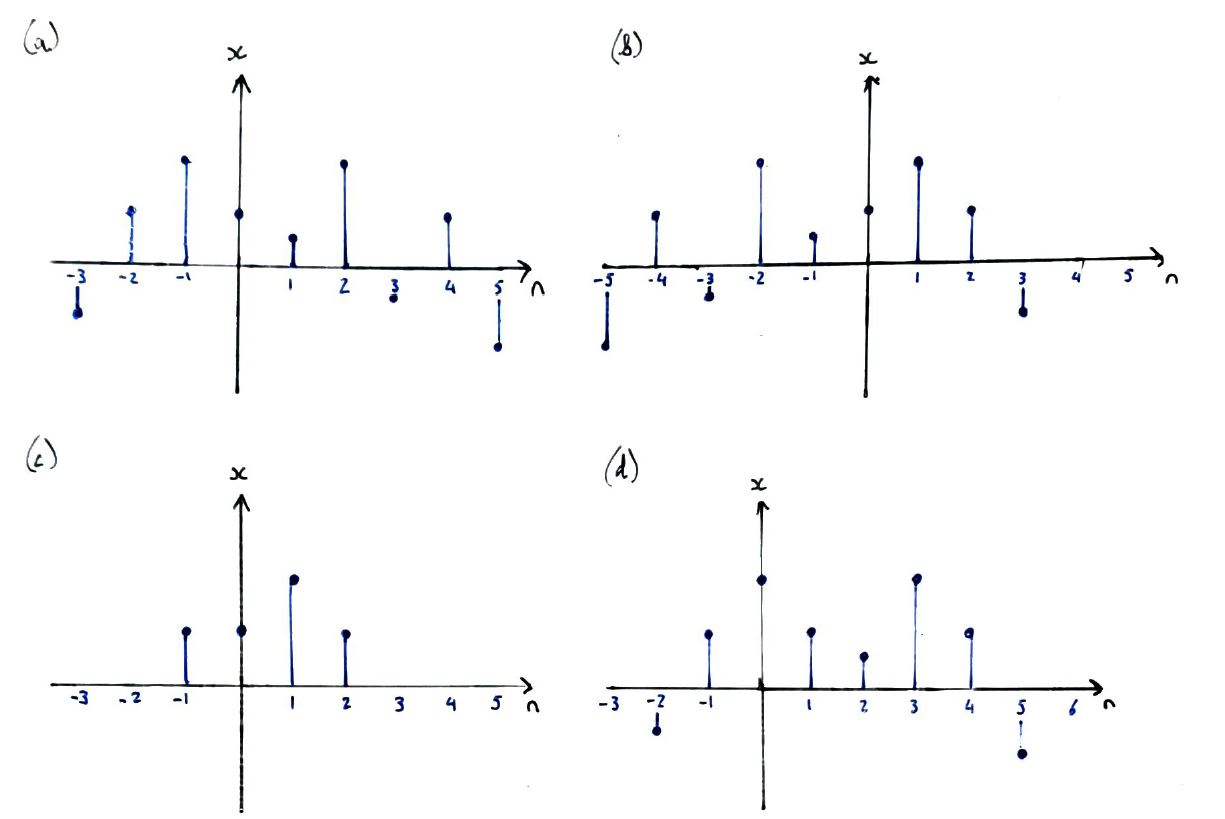
\includegraphics[width=\textwidth]{images/lecture_1_signal_operations.JPG}
  \caption{
    An example of some signals and common manipulations. (a) shows a
    signal, $x_a[n]$. (b) shows the signal from (a) having been ``reflected''
    (about the vertical axis), $x_b[n] = x_a[-n]$. (c) shows the signal from (a)
    having been ``scaled'' (in the horizontal axis), $x_c[n] = x_a[2n]$. (d) shows
    the signal from (a) having been ``shifted'' (along the horizontal axis),
    $x_d[n] = x_a[n+3]$.
  }
  \label{fig::lecture_1_signal_operations}
\end{figure}


\subsection{Compositions of Transformations}
%
The three transformations we've just discussed can be composed with general form
$n^\prime \leftarrow an + b$, where $a$ arises from the reflection and scaling (reflection
can be thought of as scaling by negative one) and $b$ arises from the shifting.
The order in which one applies these transformations is important since nonlinear algebra
is non-commutative, and can be deduced through the use of regular function composition.
Denote the reflection and scaling by $A: n\rightarrow an$ and shifting by
$B: n\rightarrow n+b$. Then,
%
\begin{displaymath}
  (B\circ A)(n) = B(an) = an + ab \,,
\end{displaymath}
%
which is clearly wrong. Exchanging the order of operations,
%
\begin{displaymath}
  (A\circ B)(n) = A(n + b) = an + b \,,
\end{displaymath}
%
as required. Consequently, transformations should be applied in the order
\textbf{shift, flip, scale}.
%
\begin{figure}[!htb]
  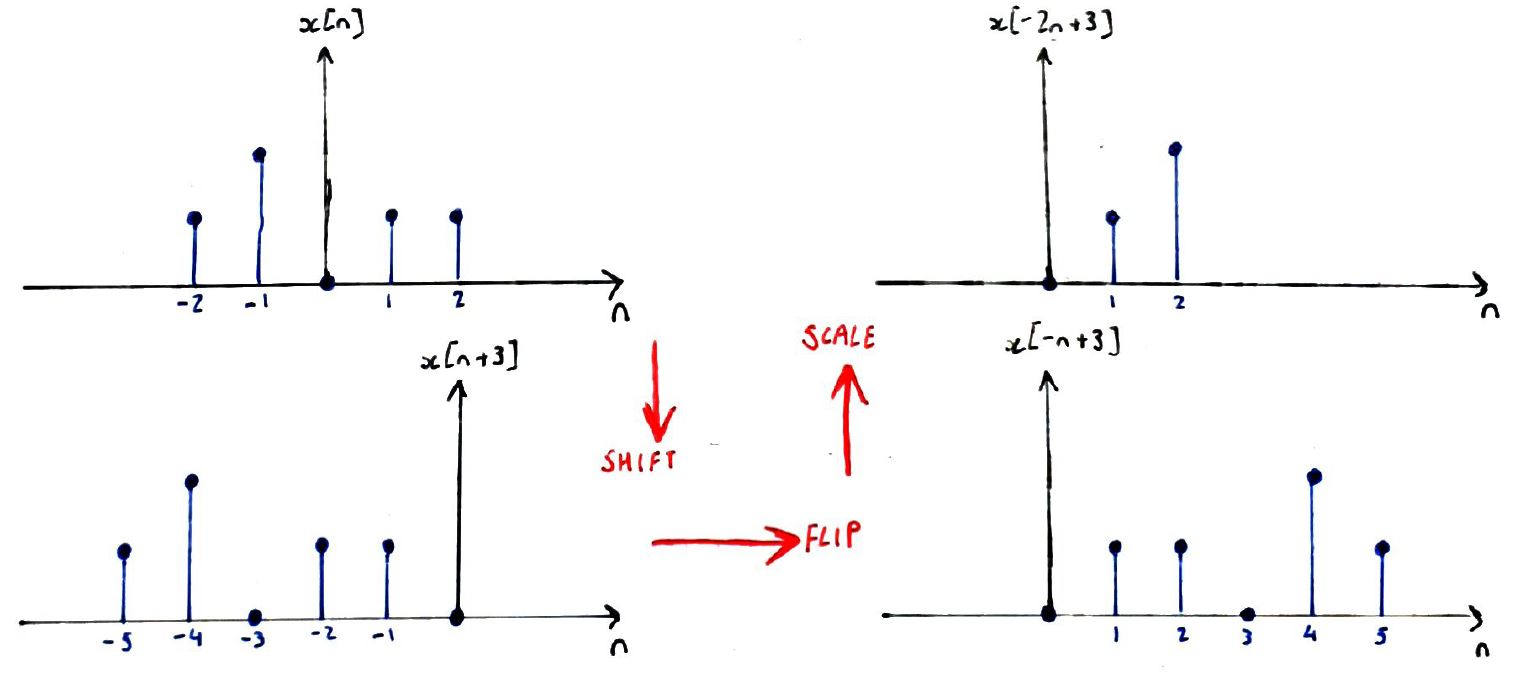
\includegraphics[width=\textwidth]{images/lecture_1_transformation_order.JPG}
  \caption{
  }
  \label{fig::lecture_1_transformation_order}
\end{figure}


\subsection{Even and Odd Functions}
%
A signal is \textbf{even} if $x[n] = x[-n]$, i.e. it is symmetric about the vertical axis.
A signal is \textbf{odd} if $x[n] = -x[-n]$, i.e. it is symmetric about the function $y = -x$.
Every signal has even and odd parts, as given by the formulae:
%
\begin{align}
  \mathrm{Even}(x[n]) &= \frac{1}{2}(x[n] + x[-n]) \,, \\
  \mathrm{Odd}(x[n]) &= \frac{1}{2}(x[n] - x[-n])  \,.
\end{align}
%
The original signal can then be recovered by adding odd and even parts. Through use of the
definitions of even and odd functions, we can verify the above representations are indeed
even and odd,
%
\begin{align*}
  \mathrm{Even}(x[n]) &= \frac{1}{2}(x[n] + x[-n]) \xrightarrow[x(n)=x(-n)]{} \frac{1}{2}(x[n] + x[-n]) \,, \\
  \mathrm{Odd}(x[n]) &= \frac{1}{2}(x[n] - x[-n]) \xrightarrow[x(n)=-x(-n)]{} \frac{1}{2}(x[n] - x[-n]) \,.
\end{align*}


\subsection{Special Signals}
%
The \textbf{delta function}, $\delta[n]$, is defined as being zero at all places where its argument
is non-zero, and one where its argument is zero,
%
\begin{equation}
  \delta[n] = \left\{\begin{array}{ccl}
    1 & & n = 0 \\
    0 & & n \neq 0
  \end{array}\right. \,.
\end{equation}
%
Note that this is simply the Kronecker delta function, where the second argument is zero, i.e. $\delta_{n0}$.
The \textbf{step function}, $u[n]$, is defined as being zero for all negative arguments and one for
all arguments that are greater than or equal to zero,
%
\begin{equation}
  u[n] = \left\{\begin{array}{ccl}
    1 & & n \geq 0 \\
    0 & & n < 0
  \end{array}\right. \,.
\end{equation}
%
\begin{figure}[!htb]
  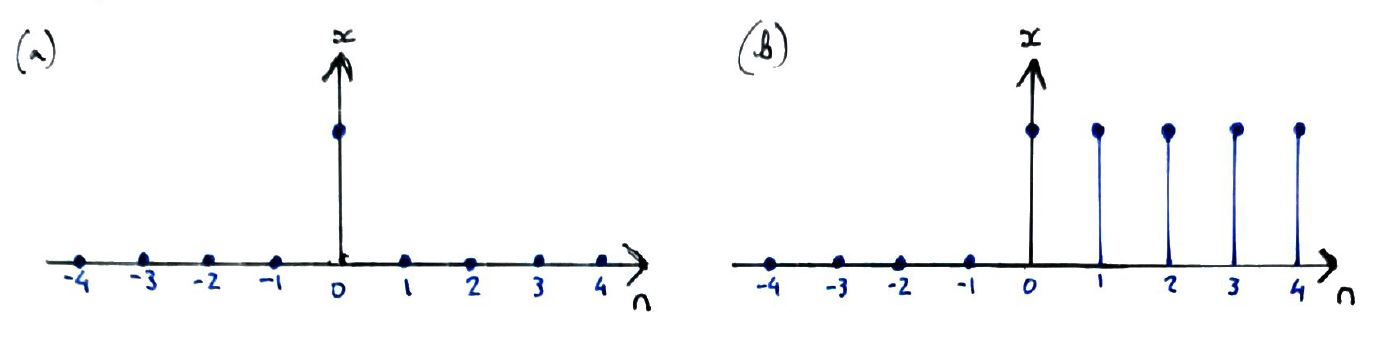
\includegraphics[width=\textwidth]{images/lecture_1_delta_and_step.JPG}
  \caption{
  }
  \label{fig::lecture_1_step_function}
\end{figure}
%
The step function can be written in terms of an infinite sum over shifted delta functions,
%
\begin{equation}
  u[n] = \delta[n] + \delta[n-1] + \delta[n-2] + \hdots = \sum_{k=0}^\infty \delta[n-k]
\end{equation}
%
In continuous-variable calculus, it can be shown that the Heaviside function, $H(t)$, (the continuous
analogue of the step function) can be written as an integral over the impulse response,
%
\begin{displaymath}
  H(t) = \int^t_{-\infty} \dx{\tau}\delta(t) \,.
\end{displaymath}
%
This integral is zero until $\tau = t$, at which point it becomes, and remains, one. In a similar
fashion, we can write the step function as a ``discrete integral'', i.e. a summation,
%
\begin{equation}
  u[n] = \sum_{k=-\infty}^n \delta[k] \,.
\end{equation}
%
One can conversely think of the delta function as the discrete derivative of the step function,
%
\begin{equation}
  \delta[n] = u[n] - u[n-1] \,,
\end{equation}
%
although note that in the discrete case, the derivative is well-defined, in contrast to the continuous
case where the derivative at the transition is undefined.\\
%
In the same way as we have created the step function from an infinite sum of shifted delta functions,
we can write any signal as an infinite sum of shifted and scaled delta functions,
%
\begin{equation}
  x[n] = \sum_{k=-\infty}^\infty \delta[n-k] x[k]
\end{equation}
%
This seems like something of a convoluted way to write out a function, but it simply allows us to
break a signal down into a sum of its component pieces using the ``sifting'' or ``sampling'' property
of the delta function, which allows us to parse out a part of a signal that we want.
%
\begin{figure}[!htb]
  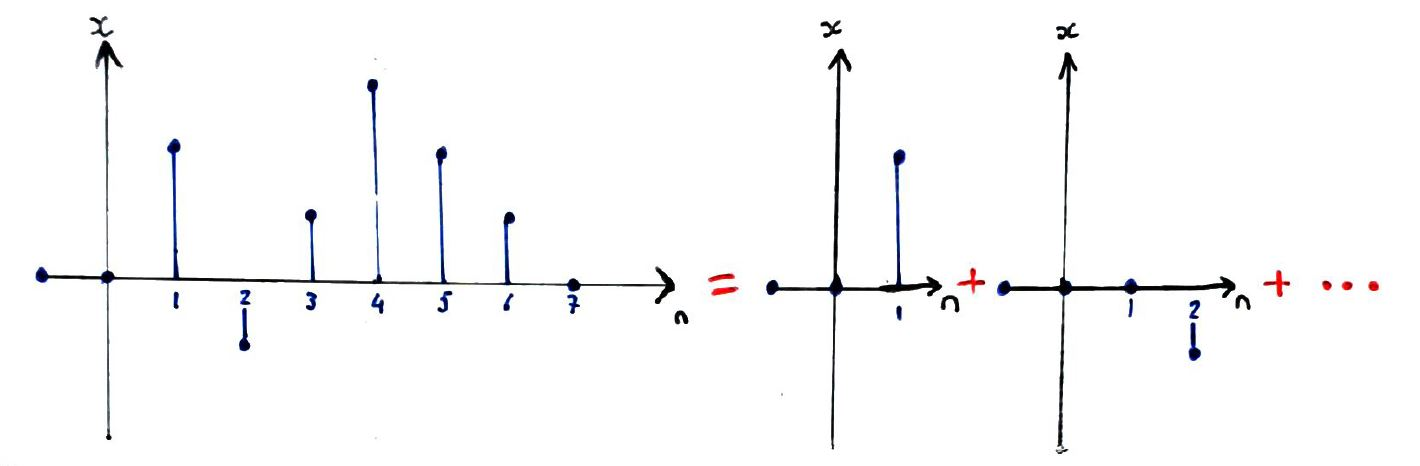
\includegraphics[width=\textwidth]{images/lecture_1_sum_of_deltas.JPG}
  \caption{
  }
  \label{fig::lecture_1_sum_of_deltas}
\end{figure}

\subsection{Complex Number Review}
%
Foregoing the basic introduction to complex numbers, we'll just recap by thinking a general complex
number, $x[t] = C\exp[at]$, where $C,a\in \mathbb{C}^2$, looks like. Writing $C = |C|\exp[\im\theta]$ in
polar form and $a = r + \im\omega_0$ in rectilinear form, we can form the expression
%
\begin{align*}
  x[t] &= C\exp[at] = |C|\exp[\im\theta]\exp[rt]\exp[\im\omega_0 t] = |C|\exp[rt]\exp[\im(\theta + \omega_0 t)] \\
  &= |C|\exp[rt]\left[ \cos(\omega_0 t + \theta) + \im\sin(\omega_0 t + \theta) \right]
\end{align*}
%
Taking the real part of $x[t]$, we see that the function is the cosine whose amplitude is bounded by the
exponential $|C|\exp[rt]$, which is either increasing or decreasing depending on whether $r$ is positive
or negative, respectively. We'll encounter many signals of this form, and referring back to its behaviour
will prove useful.
%
\begin{figure}[!htb]
  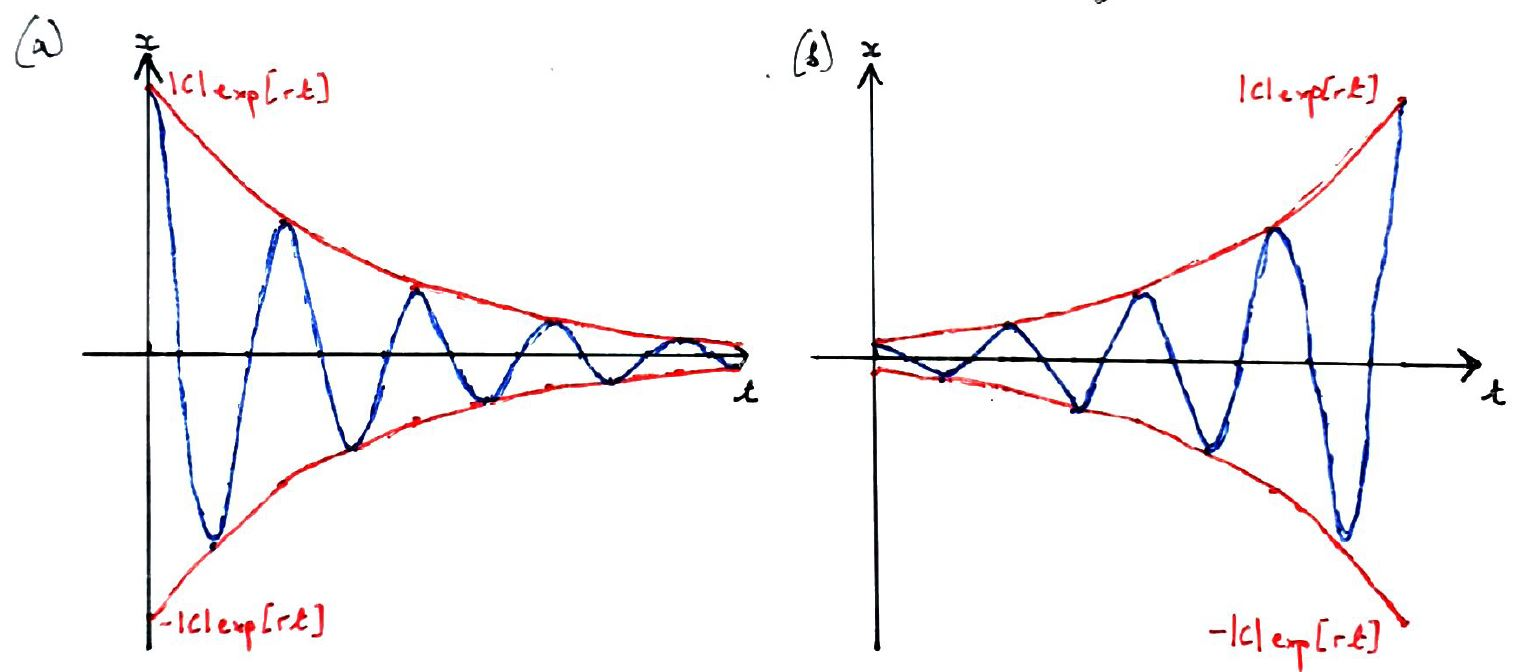
\includegraphics[width=\textwidth]{images/lecture_1_complex_numbers.JPG}
  \caption{
  }
  \label{fig::lecture_1_complex_numbers}
\end{figure}

\subsection{Periodicity in Discrete Time}
%
Consider the function $exp[\im\omega_0 n]$, a phasor rotating around the complex plane with frequency
$\omega_0$. Adding a term to $\omega_0$ results in a phasor of higher frequency. For the continuous
time case, the function $\exp[\im(\omega_0 + 2\pi)n]$ is a phasor whose frequency is $2\pi$ higher
than $\exp[\im\omega_0 n]$. However, for the discrete time case, we have that $n\in\mathbb{N}$.
Factoring our phasor,
%
\begin{displaymath}
  \exp[\im(\omega_0 + 2\pi)n] = \exp[\im\omega_0n]\exp[\im 2\pi n] = \exp[\im\omega_0n] \,.
\end{displaymath}
%
For a discrete time system, adding $2\pi$ to any frequency returns the same frequency, and
consequently there's an upper bound on the frequencies we can explore in discrete time -- that
upper bound is $\pi$ (i.e. two samples per period) since this results in
%
\begin{displaymath}
  \exp[\pi n] = \left\{\begin{array}{ccl}
  1 & & n\hspace{1mm}\mathrm{even} \\
  -1 & & n\hspace{1mm}\mathrm{odd} \\
  \end{array}\right. \,,
\end{displaymath}
%
the highest frequency with which we can recover a sinusoid -- a sampling frequency
higher than this will result in aliasing (to be covered in a later lecture).
%
\begin{figure}[!htb]
  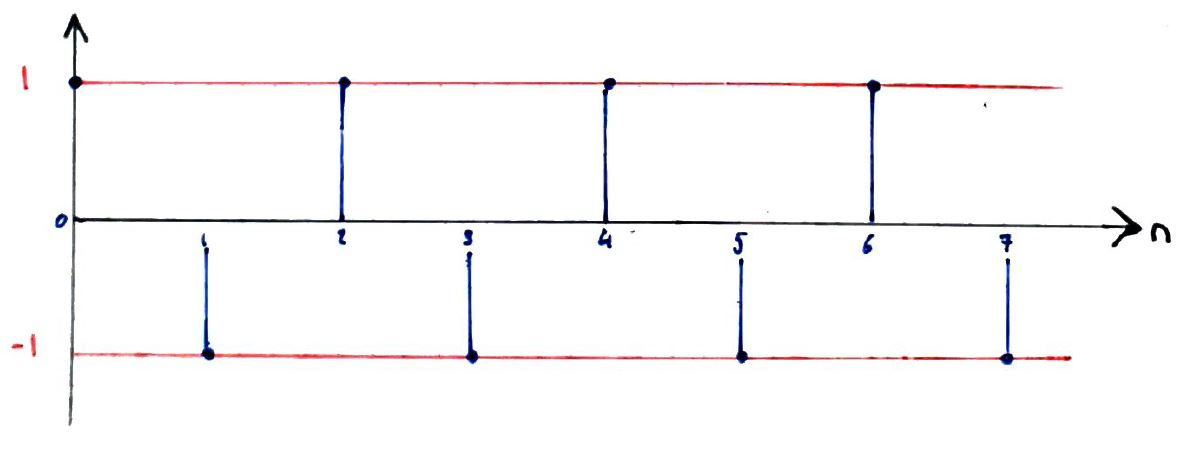
\includegraphics[width=\textwidth]{images/lecture_1_discrete_sampling.JPG}
  \caption{
  }
  \label{fig::lecture_1_discrete_sampling}
\end{figure}
%
One needs to be careful in assessing whether a signal is periodic in discrete time. It is
tempting to think that any sinusoid will surely satisfy this criterion, but this is not
the case. We need to answer when is $\exp[\im\omega_0 n]$ periodic in discrete time. By
the periodicity condition, $\exp[\im\omega_0(n+N)] = \exp[\im\omega_0n]$ for the signal
to be periodic with period $N\in\mathbb{N}$. Factoring our expression,
%
\begin{displaymath}
  \exp[\im\omega_0(n+N)] = \exp[\im\omega_0n]\exp[\im\omega_0N] \,,
\end{displaymath}
%
meaning that we require this final term to equate to one, which is satisfied when $\omega_0N$
is some multiple of $2\pi$, i.e.
%
\begin{displaymath}
  \omega_0N = 2\pi k, \qquad k\in\mathbb{N} \,.
\end{displaymath}
%
This then leads us to
%
\begin{displaymath}
  \omega_0 = \frac{2\pi k}{N} \quad\rightarrow\quad N = \frac{2\pi k}{\omega_0} \,,
\end{displaymath}
%
i.e. $N$ must be some integer multiple of $\frac{2\pi}{\omega_0}$.
%
\begin{exmp}
  Consider $x[n] = \cos[\frac{4\pi}{5}n]$.
  \begin{displaymath}
    N = \frac{2\pi k}{\omega_0} = \frac{10\pi k}{4\pi} = \frac{5}{2}k \,.
  \end{displaymath}
  Since $N,k\in\mathbb{N}$, we find that $k=2, N=5$ and the signal is periodic with
  period 5.
\end{exmp}
\begin{exmp}
  Consider $x[n] = \cos[7n]$. In continous time, this function is periodic with period
  $\frac{2\pi}{7}$. However, in discrete time,
  \begin{displaymath}
    N = \frac{2\pi k}{\omega_0} = \frac{2\pi k}{7} \,.
  \end{displaymath}
  But there is no integer $k$ which yields $N\in\mathbb{N}$ ($\pi$ is irrational, and by
  definition can't be represented as a fraction of integers), and so the signal is not
  periodic in discrete time.
\end{exmp}



\section{Lecture 2: Linear Time-Invariant Systems}

\subsection{System Properties}
%
\subsubsection{Causality}
%
The output at time $n$ only depends on the input up to time $n$. For instance,
$y[n] = x[n] - 2x[n-1]$ is causal, whereas $y[n] = x[n+3]$ is not causual.
Real-time signals are necessarily causal, whereas signals used in image processing
are not since the signal index denotes a pixel -- pixels ahead of the current
pixel are accessible at an instance of time.

\subsubsection{Linearity}
%
For a system to be linear, it must exhibit \textbf{additivity} and
\textbf{homogeneity}. Additivity requires that if $f(x_1) = y_1$ and
$f(x_2) = y_2$, then $f(x_1 + x_2) = y_1 + y_2$. Homogeneity requires that
$f(ax_1) = ay_1$ for some scalar $a$. Combining both of these properties, we can
state that linearity is given by the requirement that
%
\begin{displaymath}
  f(ax_1[n] + bx_2[n]) = ay_1[n] + by_2[n] \,,
\end{displaymath}
%
for any $x_1,x_2$.

\begin{exmp}
  Consider the function $y[n] = x[n] - 2x[n-1]$. Then, for $x_1$ and $x_2$, we have
  %
  \begin{align*}
    y_1[n] &= x_1[n] - 2x_1[n-1] \,, \\
    y_2[n] &= x_2[n] - 2x_2[n-1] \,.
  \end{align*}
  %
  The response to the input $z[n] = x_1[n] + x_2[n]$ is then
  %
  \begin{align*}
    y_z[n] = z[n] - 2z[n-1] &= (x_1[n] + x_2[n]) - 2(x_1[n-1] + x_2[n-1]) \\
    &= (x_1[n] - 2x_1[n-1]) + (x_2[n] - 2x_2[n-1) \\
    &= y_1[n] + y_2[n] \,.
  \end{align*}
  %
  Consequently, the system is additive.
\end{exmp}
%
\begin{exmp}
  Consider the same function as used in the previous example. The response to the
  input $z[n] = ax_1[n]$ is then
  %
  \begin{align*}
    y_z[n] = z[n] - 2z[n-1] &= ax_1[n] - 2ax_1[n-1] = a(x_1[n] - 2x[n-1]) \\
    &= ay_1[n] \,.
  \end{align*}
  %
  Consequently, the system is homogeneous.
\end{exmp}
%
\begin{exmp}
  Consider the function $y[n] = 3x[n] + 5$. The response to the input
  $z[n] = ax_1[n] + bx_2[n]$ is then
  %
  \begin{displaymath}
    y_z[n] = 3(ax_1[n] + bx_2[n]) + 5 \,.
  \end{displaymath}
  %
  However, $y_1[n] + y_2[n] = (3ax_1[n] + 5) + (3bx_2[n] + 5) = 3(ax_1[n] + bx_2[n]) + 10$,
  and so we fail to meet the additivity criterion. The system is then not linear.
\end{exmp}

\subsubsection{Time Invariance}
%
The system behaves the same way regardless of when the input is applied. So if
$f(x[n]) = y[n]$, then $f(x[n-n_0]) = y[n-n_0]$.
%
\begin{exmp}
  Consider the function $y[n] = x[n] - 2x[n-1]$. Then $y[n-n_0] = x[n-n_0] - 2x[n-n_0-1]$.
  We create a delayed signal $z[n] = x[n-n_0]$, such that
  %
  \begin{displaymath}
    y_z[n] = x[n-n_0] - 2x[n-n_0-1] \,,
  \end{displaymath}
  %
  which is equal to $y[n-n_0]$, and so the system is time-invariant.
\end{exmp}
%
\begin{exmp}
  Consider the function $y[n] = x[n^2]$. Then
  $y[n-n_0] = x[(n-n_0)^2] = x[n^2-2nn_0 + n_0^2]$. As before, we create a delayed signal
  $z[n] = x[n-n_0]$, such that
  %
  \begin{displaymath}
    y_z[n] = z[n^2] = x[n^2 - n_0] \,.
  \end{displaymath}
  %
  This is clearly not the same as $y[n-n_0]$, and so the system is not time-invariant.
\end{exmp}
%
A useful way to verify time-invariance is through use of the delta function. We first evaluate
the response to the input $x_1[n] = \delta[n]$, and then the response to the delayed input
$x_2[n] = \delta[n-1]$. For the function in the example above, $y[n] = x[n^2]$, we see that
the response to $x_1[n]$ yields $y_1[n] = \delta[n]$. However, QQ

\subsection{Linear Time-Invariant (LTI) Systems}
%
Real-world systems are often modelled as LTI systems since they're often a very good approximation,
and their analysis is very easy. The key concept that facilitates their treatment is that of
superposition, such that
%
\begin{equation}
  a_0x[n] + a_1x[n-1] + a_2x[n-2] + \hdots = a_0y[n] + a_1y[n-1] + a_2y[n-2] + \hdots \,.
\end{equation}
%
This is important because we strive to use the delta function, and constructing signals as
sums of shifted delta functions. The above is simply the expanded for of the sifting property
of the delta function,
%
\begin{displaymath}
  x[n] = \sum_{k=-\infty}^\infty \delta[n-k]x[k] \,,
\end{displaymath}
%
such that the response of an LTI system, $H$, to a signal $x[n]$ is given by
%
\begin{equation}
  H(x[n]) = H\left( \sum_{k=-\infty}^\infty \delta[n-k]x[k] \right) \,.
\end{equation}
%
However, the $x[k]$ are effetively constant amplitudes that scale the delta functions,
so we can invoke the linearity condition,
%
\begin{equation}
  H(x[n]) = \sum_{k=-\infty}^\infty x[k] H(\delta[n-k]) \,.
\end{equation}
%
Finally, by time-invariance,
%
\begin{equation}
  H(x[n]) = \sum_{k=-\infty}^\infty x[k] h[n-k] \,.
\end{equation}
%
This summation is a special mathematical form, referred to as convolution and denoted by
%
\begin{equation}
  y[n] = x[n] \circledast h[n] \,,
\end{equation}
%
where $h[n]$ is referred to as the unit impulse response, which fully characterises an LTI
system.

\section{Lecture 3: Convolution}

There are a number of ways in which we can manually compute the convolution
sum of the previous lecture. We'll enumerate them here. Consider the LTI system
function $y[n] = x[n] - 2x[n-1] + 3x[n-2]$, and its response to the signal
%
\begin{displaymath}
  x[n] = \left\{\begin{array}{ccl}
  1 & & 0 \leq n < 3 \\
  0 & & \mathrm{otherwise}
  \end{array}\right. \,.
\end{displaymath}

\subsection{Direct Way}
%
Since the signal is finite, we can explicity enumerate each non-zero response:
%
\begin{align*}
  y[n<0] &= 0 \\
  y[0] &= x[0] = 1 \\
  y[1] &= x[1] - 2x[0] = -1 \\
  y[2] &= x[2] - 2x[1] + 3x[0] = 2 \\
  y[3] &= -2x[2] + 3x[1] = 1 \\
  y[4] &= 3x[2] = 3 \\
  y[n>4] &= 0 \,,
\end{align*}
%
and we have $y = \left[\begin{array}{ccccc}1 & -1 & 2 & 1 & 3\end{array}\right]$.

\subsection{Convolutional Sum}
%
Recall that the convolution is given by
%
\begin{displaymath}
  y[n] = \sum_{k=-\infty}^\infty h[n-k] x[k] \,.
\end{displaymath}
%
Our first task is to compute the impulse response, $h[n]$, which is done by passing
the delta function through the system. Since the delta function just sifts the input,
$h[n]$ is given by the coefficients of the system function, i.e.
$h[0] = 1, h[1] = -2, h[2] = 3$. Expanding the summation in the convolution,
%
\begin{displaymath}
  y[n] = x[0]h[n] + x[1]h[n-1] + x[2]h[n-2] \,,
\end{displaymath}
%
and we see that we're simply weighting each of the input signal values by the
delayed impulse response (see Figure \ref{fig::lecture_3_impulse_response_weighting}).
%
\begin{figure}[!htb]
  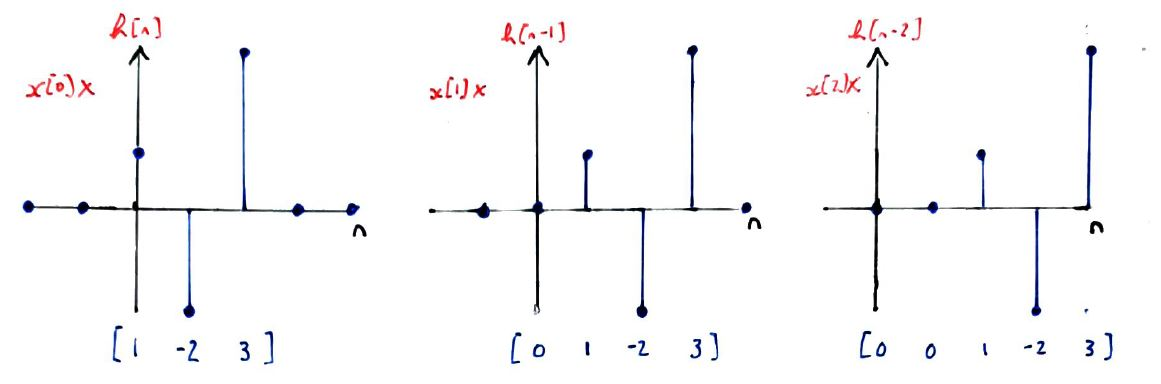
\includegraphics[width=\textwidth]{images/lecture_3_impulse_response_weighting.JPG}
  \caption{
    Each element of the signal $x[k]$ multiplies delayed versions of the impulse
    response $h[n-k]$, resulting in a partial signal. These partial signals are
    then summed to give the convolved signal, $y[n]$.
  }
  \label{fig::lecture_3_impulse_response_weighting}
\end{figure}

\subsection{``Flip and Slide''}
%
Consider the form $h[n-k]$, where $k$ is the dependent variable in our convolutional
sum. Addition of $n$ means the impulse response is first shifted to the left, and
subseqeuntly reflected about the vertical axis (see Figure
\ref{fig::lecture_3_flip_and_slide}).
%
\begin{figure}[!htb]
  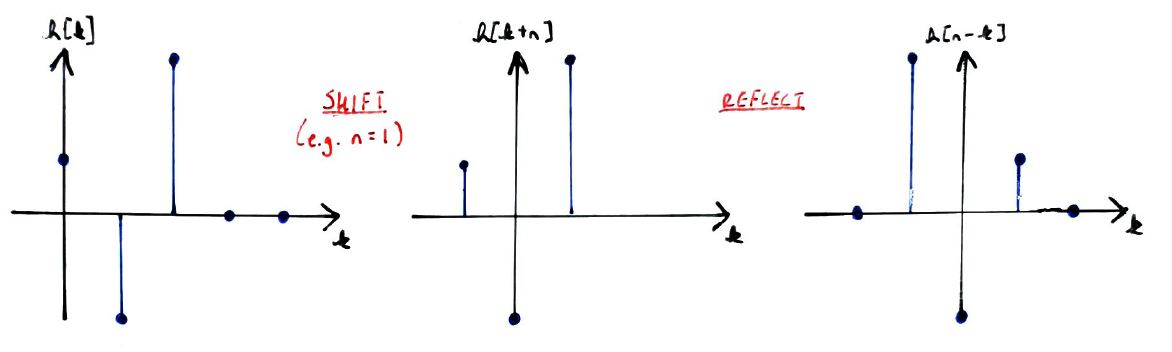
\includegraphics[width=\textwidth]{images/lecture_3_flip_and_slide.JPG}
  \caption{
    Transforming the impulse response so that it can be ``slid'' along the
    signal. Inner products with the signal then yield the convolved signal
    value at a given time.
  }
  \label{fig::lecture_3_flip_and_slide}
\end{figure}
%
The transformed impulse response is then overlapped with the input
signal and an inner product taken, yielding an element of the convolved
signal.

\subsection{Convolutional Array}
%
If it is imperative that one perform a convolution by hand, the simplest
way is probably through the use of an array like that in Figure
\ref{fig::lecture_3_convolution_grid_one}. The rows are enumerated by elements
of the impulse response and the columns by elements of the input signal.
A double line is placed under the element corresponding to the arrays
at $n=0$, and all entries in the matrix are formed by multiplying the
corresponding row and column. Diagonals are then drawn across the array
and elements on the same diagonal are summed to give the result of the
convolution.
%
\begin{figure}[!htb]
  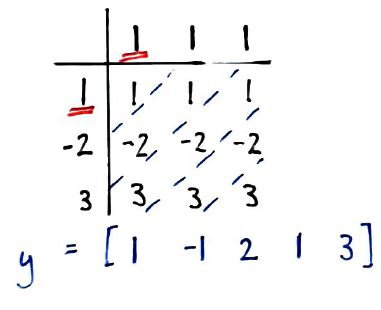
\includegraphics[width=0.3\textwidth]{images/lecture_3_convolution_grid_one.JPG}
  \caption{
    Convolutional array for the signal
    $x = \left[\begin{array}{ccc} 1 & 1 & 1\end{array}\right]$ and
    impulse response
    $h = \left[\begin{array}{ccc} 1 & -2 & 3\end{array}\right]$.
  }
  \label{fig::lecture_3_convolution_grid_one}
\end{figure}
%
In Figure \ref{fig::lecture_3_convolution_grid_one}, we have
$x = \left[\begin{array}{ccc} 1 & 1 & 1\end{array}\right]$ and
$h = \left[\begin{array}{ccc} 1 & -2 & 3\end{array}\right]$. Performing the
summation across diagonals gives the result of the convolution,
$y = \left[\begin{array}{ccccc} 1 & -1 & 2 & 1 & 3\end{array}\right]$. The
zeroth element in $y$ is given by the diagonal containing the multiplication
of underlined elements in the input array, in this case the first diagonal.

\subsection{Properties of LTI Systems}
%
\begin{enumerate}
\item An LTI system is entirely determined by its impulse response. This is \textbf{not} true
  for non-LTI systems. If it's possible to write the response to some special input, e.g. $u[n]$,
  and it is possible to write any other input in terms of this special input, then the response
  to the special input characterises the system
  \footnote{
    Adding a physical analogue for the sake of intuition, consider the problem of characterising
    the acoustics of a room. Ideally, one could produce an instantaneous sound and observe
    the acoustic response, i.e. the signal is $\delta[n]$, and the impulse response is observed.
    However, it's not possible to create a sound like $\delta[n]$ -- some finite duration must
    be associated with the noise, and so the input signal is better approximated by $u[n]$. If the
    step response can be characterised, then this can be turned into an impulse response.
  }.\\
  %
\item The convolution is commutative. This can be shown by defining the dummy dependent variable
  $m = n - k$,
  %
  \begin{align*}
    h * x &= \sum_{k=-\infty}^\infty x[k] h[n-k] = \sum_{m=-\infty}^\infty h[m] x[n-m] \\
    &= x * h \,.
  \end{align*}
  %
\item The convolution is distributive:
  %
  \begin{displaymath}
    x * (h_1 + h_2) = x * h_1 + x * h_2 \,.
  \end{displaymath}
  %
\item The convolution is associative:
  %
  \begin{displaymath}
    x * (h_1 * h_2) \Longleftrightarrow (x * h_1) * h_2 \,.
  \end{displaymath}
  %
\item For a causal system, $h[k] = 0$ for $k < 0$. This allows for a simplification in the
  form of the convolution that we've previously used through changing the lower bound of
  the summation:
  %
  \begin{equation}
    y[n] = \sum_{k=0}^\infty h[k]x[n-k] \,.
  \end{equation}
  %
  Were this not the case, $y[n]$ could depend on future values of $x$, and the system would no
  longer be causal.
\end{enumerate}
%
\begin{exmp}
  Let's begin by convolving $x[n] = \alpha^n u[n]$ with $h[n] = u[n]$, where
  $\alpha\in [0,1]$. Given the commutativity of convolution, we can effectively
  choose which function gets ``flipped and slid'' across the other. In this case,
  it will prove easiest to flip and slide the impulse response. In this way, the terms
  in the convolution turn into a geometric progression,
  %
  \begin{displaymath}
    y[-1] = 0, \quad y[0] = 1, \quad y[1] = 1 + \alpha, \quad y[2] = 1 + \alpha + \alpha^2, \hdots
  \end{displaymath}
  %
  \begin{equation}
    y[n] = \left\{\begin{array}{ccl}
    0 & & n < 0 \\
    \sum_{k=0}^n \alpha^k & & \mathrm{otherwise}
    \end{array}\right. = u[n]\sum_{k=0}^n \alpha^k \,.
  \end{equation}
  %
  Recall the elementary identity for the geometric progression when $0\leq\alpha< 1$:
  %
  \begin{displaymath}
    \sum_{k=0}^\infty \alpha^k = \frac{1}{1 - \alpha} \,.
  \end{displaymath}
  %
  For the finite sum, we can write this as
  %
  \begin{align*}
    \sum_{k=0}^n \alpha^k &= \sum_{k=0}^\infty \alpha^k - \sum_{k=n+1}^\infty \alpha^k \\
    &= \sum_{k=0}^\infty \alpha^k - \alpha^{n+1}\sum_{k=0}^\infty \alpha^k \\
    &= \frac{1}{1-\alpha} - \frac{\alpha^{n+1}}{1-\alpha} = \frac{1 - \alpha^{n+1}}{1 - \alpha} \,.
  \end{align*}
  %
  It then follows that for our convolution, we have
  %
  \begin{equation}
    y[n] = \frac{1 - \alpha^{n+1}}{1 - \alpha} u[n] \,.
  \end{equation}
  %
  This signal intercepts the vertical axis at $1$ and asymptotes to $\frac{1}{1-\alpha}$.
\end{exmp}
%
\begin{exmp}
  The previous example can actually be treated explicitly:
  %
  \begin{align*}
    y[n] &= \sum_{k=-\infty}^\infty x[k]h[n-k] = \sum_{k=-\infty}^\infty \alpha^k u[k] u[n-k] \\
    &= \sum_{k=0}^\infty \alpha^k u[n-k] = \sum_{k=0}^n \alpha^k \,,
  \end{align*}
  %
  where the second line omits the summation from $-\infty$ to $-1$ since $u[k] = 0$ for $k < 0$.
  Note that this solution makes intuitive sense: the impulse response $h[n] = u[n]$ effectively
  says that everything input to the system persists indefinitely. So we should expect the
  output at $n$ to be the partial sum of all input up to and including time $n$, as
  specified in our solution.
\end{exmp}

\section{Lecture 4: Fourier Series}

Every periodic continuous time signal can be written as a sum of sinusoids. Consider
the periodic signal $x(t)$, where
%
\begin{displaymath}
  x(t + T) = x(t), \qquad \forall t \,.
\end{displaymath}
%
The \textbf{Fourier Synthesis} allows us to represent $x(t)$ as
%
\begin{equation}
  x(t) = \sum_{k=-\infty}^\infty a_k\ex{\im k\omega_0 t} \,.
\end{equation}
%
The complex exponentials form a set of basis functions, and so we're interested in
trying to compute the expansion coefficients, $\{a_k\}$ for a given $x(t)$.
Multiplying through by $\ex{-\im n \omega_0 t}$,
%
\begin{displaymath}
  x(t)\ex{-\im n\omega_0 t} = \sum_{k=-\infty}^\infty a_k\ex{\im k\omega_0 t}\ex{-\im n\omega_0 t}
  = \sum_{k=-\infty}^\infty a_k\ex{\im (k-n)\omega_0 t} \,.
\end{displaymath}
%
Integrating both sides on the interval $[0,T]$ and factoring the $\{a_k\}$ from the integrand,
%
\begin{displaymath}
  \int_0^T \dx{t}x(t)\ex{-\im n\omega_0 t} = \sum_{k=-\infty}^\infty a_k \int_0^T\dx{t} \ex{\im (k-n)\omega_0 t} \,.
\end{displaymath}
%
Taking the integral on the right-hand side and using Euler's theorem,
%
\begin{displaymath}
  \int_0^T\dx{t} \ex{\im (k-n)\omega_0 t} = \int_0^T\dx{t} \cos((k-n)\omega_0 t) + \im\int_0^T\dx{t} \sin((k-n)\omega_0 t) \,.
\end{displaymath}
%
Taking the case where $k=n$, the first term becomes $T$ and the second term becomes zero. For the
case where $k\neq n$, we have that $(k-n)$ is an integer. Because the integral is over the time
period $T$, the integrals of the sinusoids are zero since the positive and negative regions cancel,
and consequently
%
\begin{displaymath}
  \int_0^T \dx{t} x(t)\ex{-\im n\omega_0 t} = a_n T \,,
\end{displaymath}
%
\begin{equation}
  a_n = \frac{1}{T}\int_0^T \dx{t} x(t)\ex{-\im n\omega_0 t} \,,
\end{equation}
%
which is the \textbf{Fourier Analysis}, and the $\{a_k\}$ are referred to as the Fourier series or
spectral coefficients.

\subsection{Fourier Series of Real Signals}
%
Consider the case where $x(t)$ is real. In general, the spectral coefficients are
complex, but there are some patterns that can be exploited. Take the conjugate pair
%
\begin{displaymath}
  x(t) = \sum_{k=-\infty}^\infty a_k \ex{\im k\omega_0 t}
  \quad\mathrm{and}\quad
  x^*(t) = \sum_{k=-\infty}^\infty a_k^* \ex{-\im k\omega_0 t} \,.
\end{displaymath}
%
If $x(t)$ is real, then these two expressions are, by definition, equal. In fact,
by introducing a new index,
%
\begin{displaymath}
  x^*(t) = \sum_{k=-\infty}^\infty a_k^*\ex{-\im k \omega_0 t}
  = \sum_{m=-\infty}^\infty a_{-m}^*\ex{\im m \omega_0 t} \,,
\end{displaymath}
%
we are left with the requirement that $a_k = a_{-k}^*$.\\
%
Our final relationship stems from the fact that we can eliminate the imaginary
component from the complex exponential basis functions by writing it as a cosine
alone,
%
\begin{displaymath}
  x(t) = a_0 + 2\sum_{k=1}^\infty A_k\cos(k\omega_0 t + \theta_k) \,,
\end{displaymath}
%
where the factor of two arises from the fact that $a_k = a_{-k}$, meaning the
sum from $-\infty$ to $-1$ is the same as that from $\infty$ to $1$. The amplitude
and phase, $\{A_k,\theta_k\}$ are recoverable from the spectral coefficient $a_k$.
Alternatively, we can use the double angle formula to turn the phase into
another sinusoid,
%
\begin{displaymath}
  x(t) = a_0 + 2\sum_{k=1}^\infty \left[A_k\cos(k\omega_0 t) - B_k\sin(k\omega_0 t)\right] \,.  
\end{displaymath}

\begin{exmp}
  Compute the spectral coefficients for the signal $x(t) = 5 + 2\cos(\omega_0 t)$.\\
  There's no need to undertake a full Fourier analysis here since we can
  solve by inspection. We use the identity for the cosine,
  %
  \begin{align*}
    x(t) &= 5 + 2\cos(\omega_0 t) = 5 + 2\left[
      \frac{1}{2}\ex{\im\omega_0t} + \frac{1}{2}\ex{-\im\omega_0t}
    \right] \\
    &= 5 + \ex{\im\omega_0 t} + \ex{-\im\omega_0 t} \,,
  \end{align*}
  %
  but these are simply the $\{0,1,-1\}$ terms, respectively, in the Fourier series.
  Consequently, we have $a_0 = 5, a_1 = 1, a_{-1} = 1$, and all other spectral
  coefficients are zero.
\end{exmp}

\begin{exmp}
  Consider the square wave signal in Figure \ref{fig::lecture_4_square_wave}.
  %
  \begin{figure}[H]
    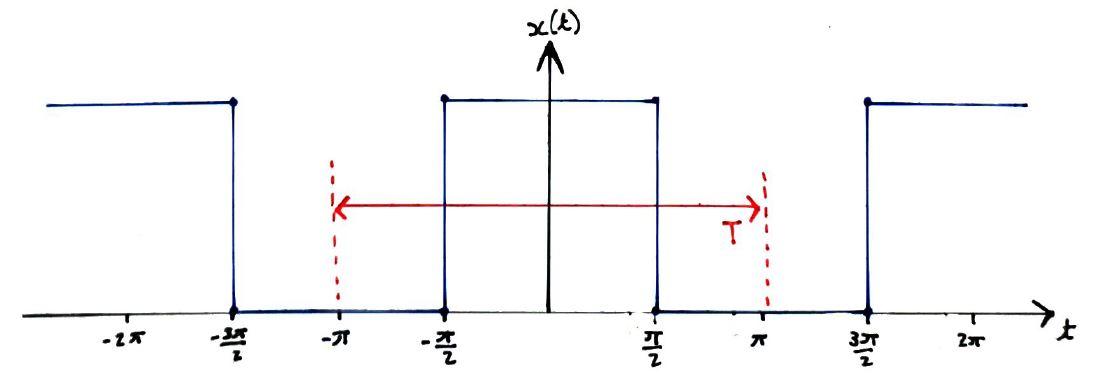
\includegraphics[width=\textwidth]{images/lecture_4_square_wave.JPG}
    \caption{
      A square wave signal of period $2\pi$, height 1 and duty cycle of $0.5$.
    }
    \label{fig::lecture_4_square_wave}
  \end{figure}
  %
  We see that it is periodic with period $T = 2\pi$, and by extension its
  angular frequency is $\omega_0 = \frac{2\pi}{T} = 1$. The zeroth spectral
  coefficient is given by the integral of the signal over its time period,
  %
  \begin{displaymath}
    a_0 = \frac{1}{T}\int_0^T\dx{t} x(t) = \frac{1}{2\pi}\times\pi = \frac{1}{2} \,.
  \end{displaymath}
  %
  For the remaining coefficients, we can integrate over any period of width $T$.
  Since the signal is even, we'll find it easier to integrate over $[-\pi,\pi]$.
  Upon further inspection, we find that this range can be reduced further to
  the non-zero regions, $[-\frac{\pi}{2},\frac{\pi}{2}]$. Now, performing the
  integration,
  %
  \begin{align*}
    a_k &= \frac{1}{T}\int_0^T\dx{t}\ex{-\im k\omega_0 t}
    = \frac{1}{2\pi}\int_{-\frac{\pi}{2}}^{\frac{\pi}{2}} \dx{t}\ex{-\im kt}
    = \left.\frac{1}{2\pi}\frac{-1}{\im k}\ex{-\im kt}\right|_{-\frac{\pi}{2}}^{\frac{\pi}{2}} \\
    &= -\frac{1}{2\pi\im k}\left(\ex{-\im k\frac{\pi}{2}} - \ex{\im k\frac{\pi}{2}}\right)
    = \frac{1}{2\pi\im k}\left(\ex{\im k\frac{\pi}{2}} - \ex{-\im k\frac{\pi}{2}}\right)
    = \frac{\sin(k\frac{\pi}{2})}{\pi k} \\
    &= \frac{1}{2}\sinc\left(\frac{k\pi}{2}\right) \,,
  \end{align*}
  %
  where we have introduced the function $\sinc(x) = \frac{\sin(x)}{x}$. Consequently,
  we can write the first few spectral coefficients,
  %
  \begin{displaymath}
    a_1 = \frac{\sin\left(\frac{\pi}{2}\right)}{\pi} = \frac{1}{\pi}, \quad
    a_2 = \frac{\sin(\pi)}{2\pi} = 0, \quad
    a_3 = \frac{\sin\left(\frac{3\pi}{2}\right)}{3\pi} = -\frac{1}{3\pi}, \quad\hdots \,.
  \end{displaymath}
\end{exmp}
%
It will be useful to have some intuition for how $\sinc(x)$ looks. It is
graphed in Figure \ref{fig::lecture_4_sinc}.
%
\begin{figure}[H]
  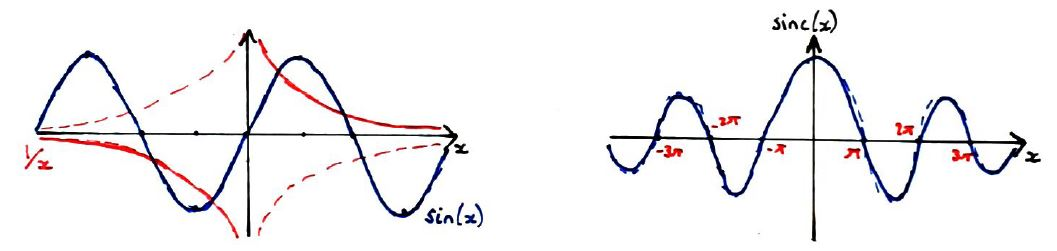
\includegraphics[width=\textwidth]{images/lecture_4_sinc.JPG}
  \caption{
    The $\sinc$ function. The important features worth keeping in mind are
    that at $\sinc(x) = 1$ at $x=0$, and the zeroes of $\sinc$ occur at
    integer multiples of $\pi$.
  }
  \label{fig::lecture_4_sinc}
\end{figure}

\subsection{Validity of the Fourier Series}
%
There are several types of function where the Fourier series doesn't really work. These
are summarised by the \textbf{Dirichlet conditions} for a real-valued periodic function. If these
conditions are satisfied, then the Fourier series converges absolutely to the
function from which it is derived.
%
\begin{enumerate}
\item The function must be square-integrable, i.e. $\int \dx{t}|x(t)|^2 < \infty$.
\item There must be a finite number of minima and/ or maxima.
\item The function must contain a finite number of discontinuities.
\end{enumerate}
%
It is interesting to consider what the Fourier series does at a discontinuity,
since it is formed by an infinite number of smooth basis functions. The Fourier
series converges absolutely at every continuous point, while it converges to the
average value of the function at a discontinuity. To see this, let's consider Figure \ref{fig::lecture_4_gibbs}.
At each discontinuity, the Fourier series yields zero, the average value of the function
at that point. Note also the overshoot in the Fourier series, referred to as the \textbf{Gibbs
Phenomenon}. This overshoot can never be less that roughly $9\%$ the height of the
discontinuity (the derivation of this quantity is fairly involved). The oscillations are
referred to as \textbf{ringing artifacts}\footnote{
  The output signal oscillates at a fading rate, much like a bell, hence ``ringing''
}, and the continual overshooting/ undershooting of the desired value is termed \textbf{clipping}. 
%
\begin{figure}[H]
  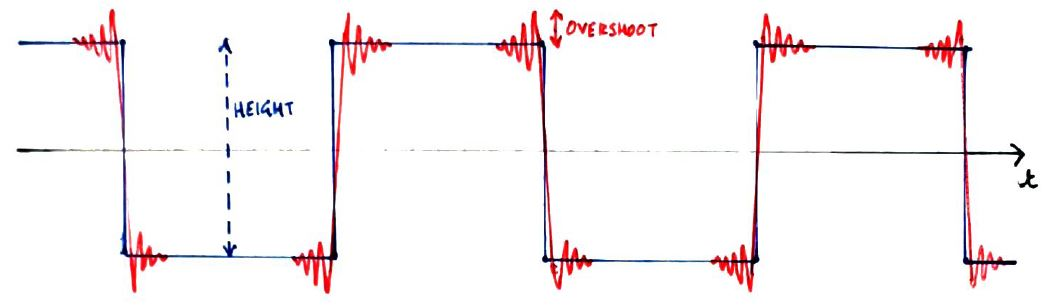
\includegraphics[width=\textwidth]{images/lecture_4_gibbs.JPG}
  \caption{
    A finite Fourier series representation of a signal. The Gibbs Phenomenon
    is clearly visible at the discontinuities.
  }
  \label{fig::lecture_4_gibbs}
\end{figure}


\subsection{Properties of the Fourier Series}
%
Suppose we have a periodic signal $x(t)$ with period $T$, whose Fourier series is given by
$\{a_k\}$. Then:
%
\begin{enumerate}
\item (\textbf{Linearity}) Given the signals $x(t) \Longleftrightarrow \{a_k\}$ and
  $y(t) \Longleftrightarrow \{b_k\}$, then
  %
  \begin{displaymath}
    \alpha x(t) + \beta y(t) \Longleftrightarrow \{\alpha a_k + \beta b_k\} \,.
  \end{displaymath}
  %
\item (\textbf{Time Shifting}) For $x(t) \Longleftrightarrow \{a_k\}$ and
  $y(t) = x(t-t_0)$, then
  %
  \begin{displaymath}
    y(t) \Longleftrightarrow \{a_k\ex{-\im k\omega_0t_0}\} \,,
  \end{displaymath}
  %
  i.e. the magnitudes of the coefficients don't change, but the phases do.
\item (\textbf{Differentiation}) For $x(t) \Longleftrightarrow \{a_k\}$,
  $x^\prime(t) \Longleftrightarrow \{\im k\omega_0 a_k\}$. This is easily shown by
  differentiating the complex exponential basis function.
\item (\textbf{Parseval's Theorem}) There is the same amount of power in both time
  and frequency domains (i.e. no information loss),
  %
  \begin{displaymath}
    \frac{1}{T}\int_0^T \dx{t} |x(t)|^2 = \sum_{k=-\infty}^\infty |a_k|^2 \,.
  \end{displaymath}
  %
\item (\textbf{Convolution}) For the signals $x(t) \Longleftrightarrow \{a_k\}$ and
  $y(t) \Longleftrightarrow \{b_k\}$,
  %
  \begin{displaymath}
    x(t)y(t) \Longleftrightarrow \sum_{m=-\infty}^\infty a_m b_{k-m} = a * b \,,
  \end{displaymath}
  %
  or conversely
  %
  \begin{displaymath}
    x* y = \int_0^T \dx{\tau} x(\tau)y(t-\tau) \Longleftrightarrow Ta_kb_k \,.
  \end{displaymath}
  %
  In other words, convolution in one domain is multiplication in the other.
\end{enumerate}

\section{Lecture 5: The Fourier Transform}

Many signals are aperiodic, i.e. the time period $T \rightarrow\infty$. Such
signals cannot be treated by the Fourier series since this results in
$\omega_0\rightarrow 0$. Consequently, our sum over sinusoids of increasing
frequency makes no sense. Rather, we need to exchange the summations for
integrations over an infinitesimal in frequency,
%
\begin{displaymath}
  x(t) = \sum_{k=-\infty}^\infty a_k\ex{\im k\omega_0 t} \xrightarrow[T\rightarrow\infty]{}
  \int\dx{\omega} \ex{\im\omega t} \times \mathrm{something} \,.
\end{displaymath}
%
\begin{figure}[!htb]
  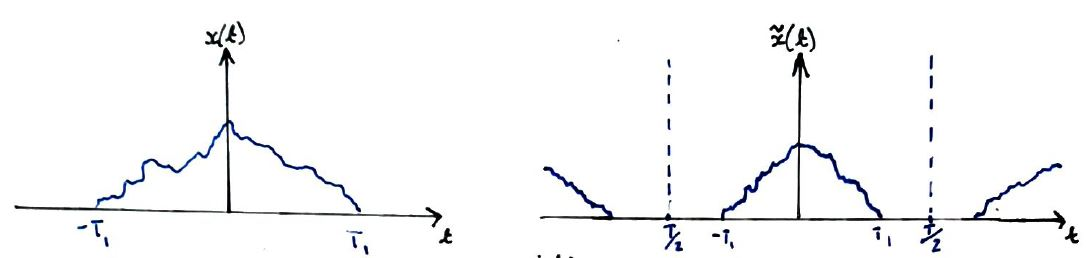
\includegraphics[width=\textwidth]{images/lecture_5_enforce_periodicity.JPG}
  \caption{
    An aperiodic signal (left) and its periodic form (right) where the time period
    has been chosen to include some time during which the signal is zero.
  }
  \label{fig::lecture_5_enforce_periodicity}
\end{figure}
%
Consider the aperiodic signal in Figure \ref{fig::lecture_5_enforce_periodicity}. We can force its periodicity (with
period $T$) by duplicating it. We'll refer to this
signal with ``enforced periodicity'' as $\tilde{x}(t)$, its Fourier synthesis
being
%
\begin{displaymath}
  \tilde{x}(t) = \sum_{k=-\infty}^\infty a_k\ex{\im k\omega_0 t} \,,
\end{displaymath}
%
and Fourier analysis
%
\begin{displaymath}
  a_k = \frac{1}{T}\int_{-T/2}^{T/2} \dx{t} \tilde{x}(t)\ex{-\im k\omega_0 t} \,.
\end{displaymath}
%
However, on the domain $t\in[-\frac{T}{2},\frac{T}{2}]$, $\tilde{x}(t)$ is simply $x(t)$.
And since this signal has no duplicates, the integral can be evaluated indefinitely
%
\begin{displaymath}
  a_k = \frac{1}{T}\int \dx{t} x(t)\ex{-\im k\omega_0 t} \,.
\end{displaymath}
%
Now, defining the \textbf{Fourier Transform} as
%
\begin{equation}
  X(\omega) = \int \dx{t} x(t)\ex{-\im\omega t} \,,
\end{equation}
%
we can formulate the Fourier coefficients
%
\begin{displaymath}
  a_k = \frac{1}{T} X(k\omega_0) \,,
\end{displaymath}
%
presenting us with the expression
%
\begin{displaymath}
  \tilde{x}(t) = \frac{1}{T}\sum_{k=-\infty}^\infty X(k\omega_0)\ex{\im k\omega_0 t} \,.
\end{displaymath}
%
Taking advantage of the fact that $\omega_0 = \frac{2\pi}{T}$,
%
\begin{displaymath}
  \tilde{x}(t) = \frac{1}{2\pi}\sum_{k=-\infty}^\infty \left[X(k\omega_0)\ex{\im k\omega_0 t}\right]\omega_0 \,.
\end{displaymath}
%
The above form allows us to gain some insight into this Fourier synthesis.
Take the example in Figure \ref{fig::lecture_5_riemann}. We see that the summation in our expression for
$\tilde{x}(t)$ is the Riemann sum, and
%
\begin{displaymath}
  \lim_{\omega_0\rightarrow 0}\tilde{x}(t) = x(t) \,.
\end{displaymath}
%
\begin{figure}[!htb]
  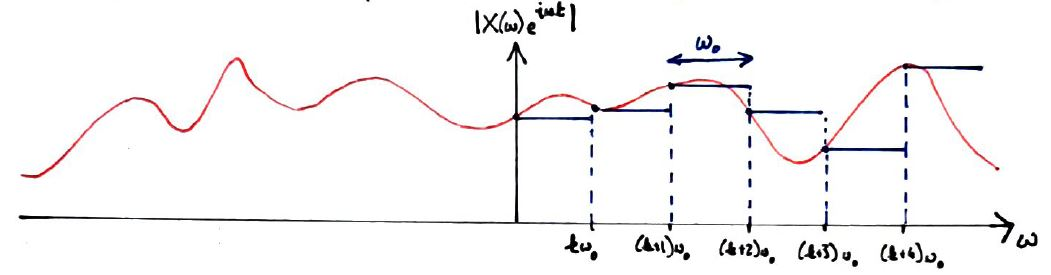
\includegraphics[width=\textwidth]{images/lecture_5_riemann.JPG}
  \caption{
    The value of the periodic signal $\tilde{x}(t)$ at time $t$ is given by the Riemann
    sum of Fourier coefficients multiplied by complex exponentials. The sum is built up
    from rectangles of width $\omega_0$ along the frequency axis. Note that the absolute
    values of the Fourier coefficients are plotted since these are complex-valued quantities.
  }
  \label{fig::lecture_5_riemann}
\end{figure}
%
Since this limit coincides with $T\rightarrow\infty$, we are effectively
pushing the duplicate copies of $x(t)$ infinitely far away, and
%
\begin{displaymath}
  \lim_{\omega\rightarrow 0}\frac{\omega_0}{2\pi}\sum_{k=-\infty}^\infty \ex{\im k\omega_0 t}
  = \frac{1}{2\pi}\int\dx{\omega}X(\omega)\ex{\im\omega t} \,.
\end{displaymath}
%
We're finally left with a pair of expressions that are the continuous-time
analogues of the Fourier synthesis and analysis:
%
\begin{align}
  x(t) &= \frac{1}{2\pi}\int\dx{\omega} X(\omega)\ex{\im\omega t} \\
  X(\omega) &= \int\dx{t} x(t)\ex{-\im\omega t} \,,
\end{align}
%
the former being the \textbf{Inverse Fourier Transform} and the latter being
the \textbf{Fourier Transform}.

\subsection{Validity of the Fourier Transform}
%
We have a similar set of criteria to those of the Fourier series regarding
the types of signals that are viable candidiates for the Fourier transform:
%
\begin{enumerate}
\item $x(t)$ must be square-integrable, i.e. $\int|x(t)|^2 < \infty$.
\item The signal must contain a finite number of extrema.
\item The signal must contain a finite number of discontinuities.
\end{enumerate}

\subsection{Some Fourier Transform Identities}
%
\begin{enumerate}
\item For the delta function, i.e. $x(t) = \delta(t)$, the Fourier transform is
  given by
  %
  \begin{displaymath}
    X(\omega) = \int \dx{t} \delta(t)\ex{-\im\omega t} = \ex{-\im\omega\times 0} = 1 \,,
  \end{displaymath}
  %
  i.e. a constant for all frequencies.
\item For the shifted delta function, i.e. $x(t) = \delta(t-t_0)$, the Fourier transform
  is given by
  %
  \begin{displaymath}
    X(\omega) = \int \dx{t} \delta(t-t_0)\ex{-\im\omega t} = \ex{-\im\omega t_0} \,.
  \end{displaymath}
  %
  These coefficients all have the same magnitude, $\sqrt{\ex{-\im\omega t_0}\ex{\im\omega t_0}} = 1$,
  but rotated on the unit circle in the complex plane, and so all have different phase.
\item For the sum of delta functions $x(t) = \delta(t-t_0) + \delta(t+t_0)$,
  %
  \begin{displaymath}
    X(\omega) = \ex{-\im\omega t_0} + \ex{-\im\omega t_0} = 2\cos(\omega t_0) \,.
  \end{displaymath}
\item For the decaying step function, $x(t) = \ex{-at}u(t)$, where $a > 0$,
  %
  \begin{align*}
    X(\omega) &= \int \dx{t} \ex{-at}u(t)\ex{-\im\omega t} = \int_0^\infty\dx{t} \ex{-t(\im\omega + a)} \\
    &= \left.-\frac{1}{(\im\omega + a)} \ex{-t(\im\omega + a)}\right|_0^\infty = \frac{1}{\im\omega + a} \,.
  \end{align*}
\item For the ``top hat'' function which is high on the domain $[-T/2,T/2]$
  %
  \begin{align*}
    X(\omega) &= \int_{-T/2}^{T/2}\dx{t}x(t)\ex{-\im\omega t} = \int_{-T/2}^{T/2}\dx{t}\ex{-\im\omega t} \\
    &= \left.-\frac{1}{\im\omega} \ex{-\im\omega t}\right|_{-T/2}^{T/2} = \frac{1}{\im\omega}
    \left(\ex{\im\omega\frac{T}{2}} - \ex{-\im\omega\frac{T}{2}}\right) \\
    &= \frac{2}{\omega}\sin\left(\omega\frac{T}{2}\right) = T\sinc\left(\frac{\omega T}{2}\right) \,.
  \end{align*}
\item For a ``top hat'' in the frequency domain which is high on the domain $[-\omega_0/2,\omega_0/2]$
  %
  \begin{align*}
    x(t) &= \frac{1}{2\pi}\int \dx{\omega}X(\omega)\ex{\im\omega t}
    = \frac{1}{2\pi}\int_{-\omega_0/2}^{\omega_0/2} \dx{\omega} \ex{\im\omega t} \\
    &= \left. \frac{1}{2\pi\im t} \ex{\im\omega t}\right|_{-\omega_0/2}^{\omega_0/2}
    = \frac{1}{2\pi\im t} \left(\ex{\im\frac{\omega_0}{2}t} - \ex{-\im\frac{\omega_0}{2}t}\right) \\
    &= \frac{\omega_0}{2\pi}\sinc\left(\frac{\omega_0}{2}t\right) \,.
  \end{align*}
  %
  This result demonstrates the duality of Fourier transform pairs -- a top hat in the
  time domain becomes a $\sinc$ in the frequency domain, and \textit{vice versa}. Similarly,
  a delta function in the time domain becomes a constant in the frequency domain and
  \textit{vice versa}.
\end{enumerate}
%
If $x(t)$ is periodic, then we can choose to use either the Fourier series or Fourier
transform. Let's choose an impulse train, $x(t) = \sum_{k=-\infty}^\infty\delta(t - kT)$,
a series of delta functions that are $T$ apart. Using the Fourier series,
%
\begin{displaymath}
  a_k = \frac{1}{T}\int_{-T/2}^{T/2}\dx{t} x(t)\ex{-\im k\frac{2\pi}{T}t} = \frac{1}{T} \,,
\end{displaymath}
%
as we have seen before since over the interval $[-T/2,T/2]$, the only non-zero point is
at $t=0$.

Suppose $x(t)$ is periodic, and consequently can be represented as a Fourier synthesis.
Then, from the Fourier transform, we have that
%
\begin{displaymath}
  X(\omega) = \int\dx{t}x(t)\ex{-\im\omega t}
  = \sum_{k=-\infty}^\infty\int\dx{t}a_k\ex{\im k\omega_0 t}\ex{-\im\omega t}
  = \sum_{k=-\infty}^\infty \int\dx{t}a_k\ex{\im (k\omega_0 - \omega) t} \,.
\end{displaymath}
%
The integral in this final expression can be simplified through use of the identity
%
\begin{displaymath}
  \int\dx{t}\ex{i(\omega - \omega_0)t} = 2\pi\delta(\omega - \omega_0) \,.
\end{displaymath}
%
This can be proven through use of a test function $G(\omega)$,
%
\begin{displaymath}
  \frac{1}{2\pi}\int\dx{\omega} G(\omega)\left(
    \int\dx{t}\ex{\im(\omega-\omega_0)t}
  \right)  = \int\dx{t}\ex{-\im\omega_0 t} \frac{1}{2\pi}\int\dx{\omega} G(\omega)\ex{\im\omega t} \,.
\end{displaymath}
%
But this second integral is simply the inverse Fourier transform of $G(\omega)$,
%
\begin{displaymath}
  \int\dx{t}\ex{-\im\omega_0 t} g(t) = G(\omega_0) \,,
\end{displaymath}
%
which is subsequently Fourier transformed, and we see that the entire operation
has simply changed the frequency variable from $\omega$ to $\omega_0$, as if
we have selected for $\omega_0$ with a delta function. Consequently, returning to
our expression for $X(\omega)$,
%
\begin{displaymath}
  X(\omega) = \sum_{k=-\infty}^\infty \int\dx{t}a_k\ex{\im (k\omega_0 - \omega) t}
  = \sum_{k=-\infty}^\infty 2\pi a_k \delta(\omega - k\omega_0) \,,
\end{displaymath}
%
where we've taken advantage of the fact that $\delta(x) = \delta(-x)$ (think about
this like a Kronecker delta: $\delta_{i,j} = \delta_{-i,-j}$). Our final form for
$X(\omega)$ lends itself to being graphed -- it's simply an infinite series of shifted
delta functions that are spaced by $\omega_0$, as can be see in Figure
\ref{fig::lecture_5_fourier_deltas}.
%
\begin{figure}[!htb]
  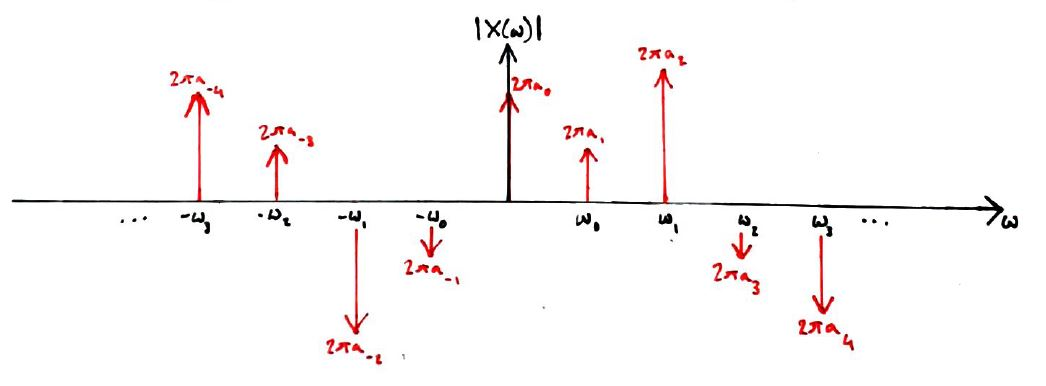
\includegraphics[width=\textwidth]{images/lecture_5_fourier_deltas.JPG}
  \caption{
    The Fourier transform of a periodic function is a series of shifted
    delta functions spaced by $\omega_0$ in the frequency domain, each one
    with magnitude $|2\pi a_k|$.
  }
  \label{fig::lecture_5_fourier_deltas}
\end{figure}

\begin{exmp}
  Consider the spectrum with $X(\pm\omega_0) = \pi$ and $X(\omega) = 0$
  for all other values of $\omega$. Conseqeuntly, we have
  %
  \begin{displaymath}
    x(t) = \frac{1}{2\pi}\int\dx{\omega}X(\omega)\ex{\im\omega t}
    = \frac{1}{2\pi} \int\dx{\omega}\delta(\omega\pm\omega_0)\ex{\im\omega t}
    = \frac{1}{2\pi}\left[\pi\ex{\im\omega_0 t} + \pi\ex{-\im\omega_0 t}\right]
    = \cos(\omega_0 t) \,,
  \end{displaymath}
  %
  which satisfies our condition of $a_k = a_{-k}$ for real-valued signals.
\end{exmp}

\subsection{Properties of the Fourier Transform}
%
\begin{enumerate}
\item (\textbf{Linearity}) Given the Fourier pairs $x(t) \Longleftrightarrow X(\omega)$ and
  $y(t) \Longleftrightarrow Y(\omega)$, then
  %
  \begin{displaymath}
    \alpha x(t) + \beta y(t) \Longleftrightarrow \alpha X(\omega) + \beta Y(\omega) \,.
  \end{displaymath}
  %
\item (\textbf{Time Shifting}) Time-shifting results in a phase change in the
  spectral coefficients, $x(t-t_0) \Longleftrightarrow X(\omega)\ex{-\im\omega t_0}$.
\item (\textbf{Real Signals}) If $x(t)$ is real, then $\Re(\omega) = \Re(-\omega)$
  and $\Im(\omega) = -\Im(-\omega)$, i.e. the real part is even and the imaginary
  part is odd.
\item (\textbf{Even and Odd Signals}) For real $x(t)$,
  $\mathrm{Even}(x(t)) \Longleftrightarrow \Re(X(\omega))$ and
  $\mathrm{Odd}(x(t)) \Longleftrightarrow \im\Im(X(\omega))$.
\item (\textbf{Differentiability})
  %
  \begin{displaymath}
    x^\prime(t) \Longleftrightarrow \im\omega X(\omega) \,,
  \end{displaymath}
  %
  \begin{displaymath}
    \int_{-\infty}^t \dx{\tau}x(\tau) \Longleftrightarrow \frac{1}{\im\omega}X(\omega) + \pi X(0)\delta(\omega) \,.
  \end{displaymath}
\item (\textbf{Scaling}) Consider $x(t) \Longleftrightarrow X(\omega)$. Then,
  %
  \begin{displaymath}
    x(at) = \frac{1}{|a|} X\left(\frac{\omega}{a}\right) \,.
  \end{displaymath}
  %
  If $a$ is large, then $x(at)$ is squeezed and $\frac{1}{|a|} X\left(\frac{\omega}{a}\right)$
  is stretched. Conversely, if $a$ is small then the opposite happens.
\end{enumerate}

\subsection{The Short-Time Fourier Transform}
%
The scaling property leads us to a rather profoud result, since it suggests
a tradeoff between our ability to simultaneously ``concentrate'' both a
function and its Fourier transform in their respective domains. This is a
result that is one of the bedrocks of quantum theory, where position and
momentum are Fourier transform pairs (to within Planck's constant), and
manifests itself as the famous Heisenberg Uncertainty Principle, where
once cannot simultaneously know both the position and momentum of a particle
to arbitrary precision. Knowledge about the particle's position to infinite
accuracy results in a complete loss of knowledge about the particle's
momentum, and \textit{vice versa}. We see that this property is the same for
the generic Fourier transform pairs we've considered in this chapter -- the
Fourier transform of a delta function is a constant across all frequency,
and \textit{vice versa}.
%
The complete derivation of the \textbf{Gabor Limit}, the maximum resolution
with which both time and frequency can be quantified in signal processing,
is presented in Section 3.11 of Brad Osgood's lecture notes on
``The Fourier Transform and its Applications'', to which the reader is
re-directed. We simply present the final result here,
%
\begin{equation}
  \sigma_t\cdot\sigma_\omega \geq \frac{1}{4\pi} \approx \textrm{0.08\;Cycles} \,,
\end{equation}
%
where $\sigma_t, \sigma_\omega$ are the standard deviations in the time and
frequency domains, respectively.

This Gabor limit presents us with an opportunity in signal processing. For a
complex time domain signal, different frequencies appear at different times.
Consider the example of playing an instrument -- in a simplistic sense,
this is simply a sequence of notes, or discrete frequencies, in time. Yet, if
we take the Fourier transform of an audio recording of the piece, all we can
see is that these discrete frequencies were present in the time-domain signal,
it tells us nothing about when in the piece the frequencies were active. In
effect, we're presented with either an infinite precision in the time domain
(the audio track) or an infinite precision in the frequency domain (the
Fourier transform). And this is where the Gabor limit becomes important -- in
principle, I can work out a little bit about both, as long as the product
of standard deviations in time and frequency do not exceed $\frac{1}{4\pi}$.\\

One method for generating a \textbf{spectrogram}, a plot of time against
frequency upon which magnitudes are plotted (i.e. how ``active'' a certain
frequency is at a certain point in time) is the is the
\textbf{Short-Time Fourier Transform} (STFT). 

\section{Lecture 6: The Frequency Response}

We have seen that the output of a system is given from the
convolution of an input signal and the system's impulse response
%
\begin{displaymath}
  y(t) = x(t) * h(t) = \int\dx{\tau}x(\tau)h(t-\tau) \,.
\end{displaymath}
%
We have also seen from our study of the Fourier series that a
convolution in the time domain becomes a multiplication in the
frequency domain. We can show this holds for the Fourier transform
%
\begin{align*}
  Y(\omega) &= \int\dx{t} y(t)\ex{-\im\omega t}
  = \int\dx{t}\ex{-\im\omega t}\left[\int\dx{\tau}x(\tau)h(t-\tau)\right]
  = \int\dx{\tau}x(\tau)\left[\int\dx{t}h(t-\tau)\ex{-\im\omega t}\right] \\
  &= \int \dx{\tau}x(\tau)\mathscr{F}\left[h(t-\tau)\right] \,,
\end{align*}
%
where $\mathscr{F}$ denotes a Fourier transform. From the time-shifting
property of the Fourier transform established in the previous lecture,
this conveniently becomes
%
\begin{align*}
  Y(\omega) &= \int \dx{\tau}x(\tau)\mathscr{F}\left[h(t-\tau)\right]
  = \int \dx{\tau}x(\tau)H(\omega)\ex{-\im\omega\tau} \\
  &= \mathscr{F}\left[x(\tau)\right]H(\omega) = X(\omega)H(\omega) \,,
\end{align*}
%
as required.\\

From our earlier treatment of LTI systems, we know that the convolution
is important since the impulse response fully characterises the system.
The Fourier transform of this quantity, $H(\omega)$, is referred to as
the \textbf{frequency response}.

\subsection{What Does the Frequency Response Mean?}
%
%
The frequency response takes every subcomponent frequency of the input and
modulates it by some amplitude and shifts it by some phase. So the value of the
frequency response at some fixed frequency tells us how the sinusoid of that
frequency is being modified by the system. Let's verify this using the
generic signal $x[n] = A\ex{\im\omega_0 n}$:
%
\begin{align*}
  y[n] &= \infsum{k}h[k]x[n-k] = A\infsum{k}h[k]\ex{\im\omega_0(n-k)} \\
  &= A\ex{\im\omega_0 n}\infsum{k}h[k]\ex{-\im\omega_0 k} = H(\omega_0)A\ex{\im\omega_0 n} \,,
\end{align*}
%
i.e. given an input complex exponential, we get the same one back modulated by
some complex number $H(\omega_0)$. Putting $H(\omega_0)$ in polar form
%
\begin{displaymath}
  A\ex{\im\omega_0 n} \quad\rightarrow\quad
  |H(\omega_0)|A\ex{\im\theta_0}\ex{\im\omega_0 n} \quad\rightarrow\quad
  |H(\omega_0)|A\ex{\im(\omega_0 n + \theta_0)} \,.
\end{displaymath}
%
where $|H(\omega_0)|$ is the amplitude scale and $\theta_0$ is the phase
shift for the frequency $\omega_0$.
%
\begin{exmp}
  Suppose $h(t)$ is real and $x(t) = \cos(\omega_0 t)$. We saw in the previous
  lecture that $X(\omega_0) = \pi[\delta(\omega-\omega_0) + \delta(\omega+\omega_0)]$.
  Then
  %
  \begin{align*}
    Y(\omega) &= \pi[\delta(\omega-\omega_0) + \delta(\omega+\omega_0)]H(\omega) \\
    &= \pi[\delta(\omega-\omega_0)H(\omega_0) + \delta(\omega+\omega_0)H(-\omega_0)]
    = \pi[\delta(\omega-\omega_0)H(\omega_0) + \delta(\omega+\omega_0)H^*(\omega_0)] \,,
  \end{align*}
  %
  where the second line uses the filtering of the delta function to select those
  values of the frequency response where the delta function fires, and the final
  equality results from $H(-\omega_0) = H^*(\omega_0)$ as a result of $x(t)$ being
  real. Now expressing the frequency response in polar form,
  %
  \begin{displaymath}
    Y(\omega) = \pi |H(\omega_0)|\left[
      \ex{\im\theta}\delta(\omega-\omega_0) + \ex{-\im\theta}\delta(\omega+\omega_0)
    \right] \,,
  \end{displaymath}
  %
  where $\theta$ is the phase of $H(\omega_0)$. Transforming this back into the time
  domain,
  %
  \begin{align*}
    y(t) &= \frac{1}{2\pi}\int\dx{\omega}Y(\omega)\ex{\im\omega t} \\
    &= \frac{|H(\omega_0)|}{2} \left[
      \ex{\im\theta}\ex{\im\omega_0 t} + \ex{-\im\theta}\ex{-\im\omega_0 t}
      \right] = \frac{|H(\omega_0)|}{2} \left[
      \ex{\im(\omega_0 t + \theta)} + \ex{-\im(\omega_0 t + \theta)}
      \right] \\
    &= |H(\omega_0)|\cos(\omega_0 t + \theta) \,.
  \end{align*}
  %
  We see that the frequency content of the signal has not changed -- only the phase
  has changed. If a system changes the frequency of an input, it is not an LTI system.
\end{exmp}
%
\begin{exmp}
  Consider the impulse response $h[n] = \left(\frac{1}{3}\right)^n u[n]$ and input
  signal $x[n] = 2\ex{\im\frac{\pi}{3}n}$. $x[n]$ is a single sinusoid at frequency
  $\pi/3$, so we only need to know what the frequency response does at this value:
  %
  \begin{displaymath}
    H(\omega) = \frac{1}{1 - \frac{1}{3}\ex{-\im\omega}} \quad\Longrightarrow\quad
    H\left(\frac{1}{3}\right) = \frac{1}{1 - \frac{1}{3}\ex{-\im\frac{\pi}{3}}}
    = \frac{1}{\frac{5}{6} + \frac{\sqrt{3}}{6}\im} \,,
  \end{displaymath}
  %
  and consequently we have
  %
  \begin{displaymath}
    y[n] = 2 \left|H\left(\frac{\pi}{3}\right)\right| \ex{\im\left(\frac{n\pi}{3} + \theta\right)} \,.
  \end{displaymath}
  As a result, we see that there's no need to take $x[n]$ into the frequency domain.
\end{exmp}

\subsection{Filters}
%
We typically interpret $H(\omega)$ as what the system does to frequencies of the
input signal, \textbf{filter} being a common synonym. The most important of these
is the low-pass filter which is depicted in Figure \ref{fig::lecture_6_low_pass_filter}.
This is a top hat function in the frequency domain whose edges are at $\pm\omega_c$, the
\textbf{cutoff frequency}. The frequency response filters our all frequencies
outside of the cutoff frequency. From the form of the frequency response, we can
conclude that $h(t)$ takes the form of a $\sinc$ with nodes at $n\pi/\omega_c$, where
$n$ is an integer, and height $h(0) = \omega_c/\pi$, i.e.
$h(t) = \frac{\omega_c}{\pi}\sinc(\omega_c t)$.
%
\begin{figure}[!htb]
  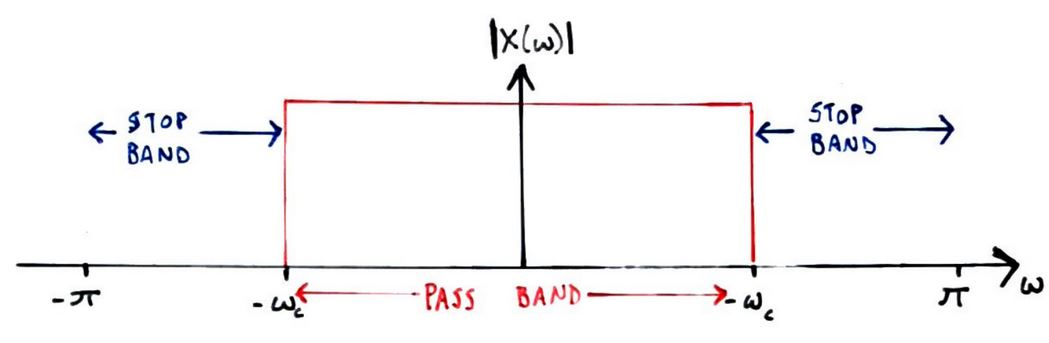
\includegraphics[width=\textwidth]{images/lecture_6_low_pass_filter.JPG}
  \caption{
  }
  \label{fig::lecture_6_low_pass_filter}
\end{figure}
%
There are, however, issues with implementing $h(t)$. For one, it is not causal
since the $\sinc$ is symmetric, and $h(t<0) \neq 0$. It also extends
\textit{ad infinitum} in time, and consequently trucations result in errors.
%
\begin{exmp}
  Consider the impulse response $h(t) =\ex{-at}u(t)$ for $a>0$. We have previously
  found that $\mathscr{F}[h(t)] = \frac{1}{a + \im\omega}$. So,
  %
  \begin{displaymath}
    |H(\omega)| = \sqrt{\frac{1}{(a + \im\omega)(a - \im\omega)}}
    = \frac{1}{\sqrt{a^2 + \omega^2}} \,,
  \end{displaymath}
  %
  which intercepts the vertical axis at $1/a$ and decays like $1/\omega^2$ for
  large $\omega$ -- it resembles a Gaussian. Consequently, $h(t)$ offers
  a fairly crude approximation to a low-pass filter.
\end{exmp}

\subsection{Solving LTI Systems}
%
The most straightforward way to solve a LTI system is to first compute
$X(\omega)$ from $x(t)$, and then multiply it by $H(\omega)$ to yield
$Y(\omega)$. Finally, we perform an inverse Fourier transform to get
$y(t)$.
%
\begin{exmp}
  Consider the signal $x(t) = \ex{-5t}u(t)$ and $h(t) = \ex{-3t}u(t)$.
  Then we have
  %
  \begin{displaymath}
    X(\omega) = \frac{1}{5 + \im\omega} \hspace{10mm}
    H(\omega) = \frac{1}{3 + \im\omega} \,.
  \end{displaymath}
  %
  As a result,
  %
  \begin{align*}
    Y(\omega) &= \frac{1}{(5 + \im\omega)(3 + \im\omega)}
    = \frac{A}{5 + \im\omega} + \frac{B}{3 + \im\omega}
    = \frac{A(3+\im\omega) + B(5+\im\omega)}{(5+\im\omega)(3+\im\omega)} \\
    &= \frac{(3A + 5B) + (A+b)\im\omega}{(5+\im\omega)(3+\im\omega)} \,.
  \end{align*}
  %
  Comparing with out actual expression and equating coefficients, we then
  have $(3A + 5B) = 1, (A + B) = 0$. As such, $A=1/2$ and $B=-1/2$, leading
  us to the output
  %
  \begin{displaymath}
    Y(\omega) = \frac{1}{2(3+\im\omega)} - \frac{1}{2(5+\im\omega)} \,,
  \end{displaymath}
  %
  and since the Fourier transform is linear,
  %
  \begin{displaymath}
    y(t) = \frac{1}{2}\ex{3t}u(t) - \frac{1}{2}\ex{5t}u(t) \,.
  \end{displaymath}
\end{exmp}
%
Fourier techniques can also be used to simplify the solution to differential
equations.
%
\begin{exmp}
  Consider the ODE
  %
  \begin{displaymath}
    \frac{\dsqx{{y}(t)}}{\dx{t}^2} + 4\frac{\dx{y}(t)}{\dx{t}} + 3y(t)
    = \frac{\dx{x}(t)}{\dx{t}} + 2x(t) \,.
  \end{displaymath}
  %
  From the dual $y(t) = x^\prime(t) \Longleftrightarrow Y(\omega) = \im\omega X(\omega)$,
  %
  \begin{displaymath}
    (\im\omega)^2 Y(\omega) + 4\im\omega Y(\omega) + 3Y(\omega)
    = \im\omega X(\omega) + 2X(\omega) \,.
  \end{displaymath}
  %
  Then we can construct the frequency response from the coefficients
  %
  \begin{displaymath}
    H(\omega) = \frac{Y(\omega)}{X(\omega)}
    = \frac{2 + \im\omega}{(1+\im\omega)(3+\im\omega)} \,,
  \end{displaymath}
  %
  which allows us to evaluate $Y(\omega)$ for any $X(\omega)$.
\end{exmp}

\section{Lecture 7: The Discrete-Time Fourier Transform}

We begin by defining the \textbf{discrete-time Fourier transform} (DTFT)
%
\begin{equation}\label{eq::lecture_7_dtft}
  X(\omega) = \sum_{n=-\infty}^\infty x[n]\ex{-\im\omega n} \,.
\end{equation}
%
Note that while this expression is discrete in time, it is continuous
in frequency. However, while the continuous-time Fourier transform
has the frequency range $[-\infty,\infty]$, the DTFT is $2\pi$-periodic
as we've previously pointed out,
%
\begin{displaymath}
  X(\omega + 2\pi) = \sum_{n=-\infty}^\infty x[n]\ex{-\im(\omega+2\pi)n}
  = \sum_{n=-\infty}^\infty x[n]\ex{-\im\omega n}\ex{-\im 2\pi n}
  = \sum_{n=-\infty}^\infty x[n]\ex{-\im\omega n} = X(\omega) \,.
\end{displaymath}
%
So while the DTFT can be evaluated at any frequency, we must exercise
caution in only concerning ourselves with the range $[-\pi,\pi]$.
We'll also introduce the \textbf{discrete-time inverse Fourier transform}
(IDTFT) as
%
\begin{equation}
  x[n] = \frac{1}{2\pi}\int_{-\pi}^\pi\dx{\omega} X(\omega)\ex{\im\omega n} \,.
\end{equation}
%
We can prove that this is the inverse of \eqref{eq::lecture_7_dtft} by
%
\begin{align*}
  x[n] &= \frac{1}{2\pi}\int_{-\pi}^\pi\dx{\omega} X(\omega)\ex{\im\omega n}
  = \frac{1}{2\pi}\int_{-\pi}^\pi\dx{\omega} \sum_{m=-\infty}^\infty x[m]\ex{-\im\omega m}\ex{\im\omega n} \\
  &= \sum_{m=-\infty}^\infty \frac{x[m]}{2\pi}\int_{-\pi}^\pi\dx{\omega}\ex{\im\omega(n-m)}
  = \sum_{m=-\infty}^\infty \frac{x[m]}{2\pi}\delta_{mn}2\pi \\
  &= x[n] \,,
\end{align*}
%
as required. However, note that a sufficient condition for the interchange of
summation and integration on the second line is that $\sum_n|x[n]| < \infty$,
as per the Fubini-Tonelli theorem.
%
\begin{exmp}
  Consider the frequency response given by the top hate which is high over the
  interval $[-\omega_c,\omega_c]$, where $\omega_c < \pi$. Then
  %
  \begin{align*}
    x[n] &= \frac{1}{2\pi}\int_{-\pi}^\pi \dx{\omega}X(\omega)\ex{-\im\omega n}
    = \frac{1}{2\pi}\int_{-\omega_c}^{\omega_c} \dx{\omega}\ex{-\im\omega n}
    = \left. \frac{1}{2\pi\im n}\ex{-\im\omega n}\right|_{-\omega_c}^{\omega_c} \\
    &= \frac{1}{2\pi\im n} \left(\ex{\im\omega_c n} - \ex{-\im\omega_c n}\right)
    = \frac{1}{\pi n}\sin(\omega_c n) = \frac{\omega_c}{\pi}\sinc(\omega_c n) \,.
  \end{align*}
  %
  This function satisfies $\sum_n|x[n]|^2 < \infty$, but not $\sum_n|x[n]| < \infty$,
  which manifests itself as the Gibbs phenomenon since the interchange of summation
  and integration that was invoked in the proof of the IDTFT is no longer valid.
\end{exmp}
%
\begin{exmp}
  Let
  %
  \begin{displaymath}
    x[n] = \delta[n] \Longleftrightarrow X(\omega)
    = \sum_{n=-\infty}^\infty\delta[n]\ex{-\im\omega n} = 1 \,.
  \end{displaymath}
  %
  Now consider $X(\omega) = \delta(\omega)$. Recall that the DTFT is
  $2\pi$-periodic. What we mean by $X(\omega) = \delta(\omega)$ is that
  there is a delta function at every interval of $2\pi$:
  %
  \begin{displaymath}
    X(\omega) = \delta(\omega) \Longleftrightarrow x[n]
    = \frac{1}{2\pi}\int_{-\pi}^\pi\dx{\omega}X(\omega)\ex{\im\omega n} = \frac{1}{2\pi} \,.
  \end{displaymath}
  %
  So a delta function in the frequency domain is a constant in the time
  domain, and \textit{vice versa}, as before.
\end{exmp}
%
\begin{exmp}
  Consider a pulse in the time domain,
  %
  \begin{displaymath}
    x[n] = \left\{\begin{array}{ccl}
    1 & & -m \leq n \leq m \\
    0 & & \mathrm{otherwise}
    \end{array}\right. \,.
  \end{displaymath}
  %
  From the continuous Fourier transform of the top hat function, we expect
  something like a $\sinc$ for the DTFT. But $\sinc$ is not periodic, let alone
  $2\pi$-periodic. Consequently, we expect something like $\sinc$, but $2\pi$-periodic.
  The DTFT is
  %
  \begin{displaymath}
    \infsum{n}x[n]\ex{-\im\omega n} = \sum_{n=-m}^m \ex{-\im\omega n}
    = \ex{\im\omega m}\sum_{n=0}^{2m}\ex{-\im\omega n} \,.
  \end{displaymath}
  %
  With a little foresight, we'll find it prudent to evaluate
  $X(0) = 2m + 1$ before simplifying further. Next, from a table of finite sum
  expressions, we have
  %
  \begin{displaymath}
    \ex{\im\omega m}\sum_{n=0}^{2m}\ex{-\im\omega n}
    = \ex{\im\omega m}\left(
    \frac{1 - \ex{-\im\omega(2m+1)}}{1 - \ex{-\im\omega}}
    \right) \,.
  \end{displaymath}
  %
  Note that this expression is undefined at $\omega = 0$. We can force some
  sinusoids to appear in this expression by factoring out $\ex{-\im\omega\frac{2m+1}{2}}$
  in the numerator and $\ex{-\frac{\im\omega}{2}}$,
  %
  \begin{align*}
    X(\omega) &= \ex{\im\omega m}\left(
    \frac{1 - \ex{-\im\omega(2m+1)}}{1 - \ex{-\im\omega}}
    \right)
    = \ex{\im\omega m}\left(
    \frac{\ex{-\im\omega\frac{2m+1}{2}}\left(\ex{\im\omega\frac{2m+1}{2}}
        - \ex{-\im\omega\frac{2m+1}{2}}\right)}{\ex{-\frac{\im\omega}{2}}\left(\ex{\frac{\im\omega}{2}}
      - \ex{-\frac{\im\omega}{2}}\right)}
    \right) \\
    &= 
    \frac{
      \ex{\im\omega\frac{2m+1}{2}} - \ex{-\im\omega\frac{2m+1}{2}}
    }{
      \ex{\frac{\im\omega}{2}} - \ex{-\frac{\im\omega}{2}}
    } 
    = \frac{\sin\left(\omega\frac{2m+1}{2}\right)}{\sin\left(\frac{\omega}{2}\right)} \,.
  \end{align*}
  %
  This indeed looks like $\sinc$, but from Figure QQ we see it has
  $2\pi$-periodicity as required.
\end{exmp}
%
We have seen for the continuous-time Fourier transform that
$x(t) * h(t) \Longleftrightarrow X(\omega)H(\omega)$. This still holds for the DTFT
as shown here:
%
\begin{align*}
  Y(\omega) &= \infsum{n}y[n]\ex{-\im\omega n} = \infsum{n}\infsum{k}x[k]h[n-k]\ex{-\im\omega n} \\
  &= \infsum{k}x[k]\infsum{n}h[n-k]\ex{-\im\omega n} = \infsum{k}x[k]\infsum{m}h[m]\ex{-\im\omega(m + k)} \\
  &= \infsum{k}x[k]\ex{-\im\omega k}\infsum{m}h[m]\ex{-\im\omega m} 
  = \infsum{k}x[k]\ex{-\im\omega k} H(\omega) \\
  &= X(\omega)H(\omega) \,.
\end{align*}

\subsection{Magnitude and Phase Responses}
%
\begin{exmp}
  Let $x[n] = a^n u[n]$ for $|a|>0$. Then,
  %
  \begin{displaymath}
    X(\omega) = \infsum{k}a^n u[n]\ex{-im\omega n} = \sum_{k=0}^\infty a^n\ex{-\im\omega n}
    = \sum_{n=0}^\infty\left(a\ex{-\im\omega}\right)^n \,.
  \end{displaymath}
  %
  This series is strictly decreasing, and so must be absolutely summable and
  hence can be represented by the DTFT. In this case, we have the geometric series
  %
  \begin{displaymath}
    X(\omega) = \sum_{n=0}^\infty\left(a\ex{-\im\omega}\right)^n = \frac{1}{1-a\ex{-\im\omega}} \,.
  \end{displaymath}
  %
  Note that this expression is complex-valued, and so we conclude as for the continuous
  time case that a real-valued signal yields a complex DTFT. It's convenient to be
  able to plot such complex-valued expressions, and so we plot the
  \textbf{magnitude response},
  %
  \begin{displaymath}
    |X(\omega)| = \left|\frac{1}{1-a\ex{-\im\omega}}\right|
    = \sqrt{\frac{1}{(1-a\ex{-\im\omega})(1-a\ex{\im\omega})}}
    = \frac{1}{\sqrt{1 + a^2 - 2a\cos(\omega)}} \,.
  \end{displaymath}
  %
  Some useful points on here include $|X(0)| = \frac{1}{1-a}$ and 
  $|X(\pm\pi)| = \frac{1}{1+a}$. The function resembles that of the frequency
  response of a decaying exponential as discussed in the previous lecture.
\end{exmp}
%
Typically, filters are named based on how their magnitude response looks. Some
``ideal filters'' are presented in Figure QQ.
%
The \textbf{phase response} is also an important quantity -- it transpires that
a desirable phase response is of the form $\theta = -c\omega$, where $c$ is some
constant. Consider a piecewise constant $\left|H(\omega)\right|$ as seen in
the ideal filters. In the pass region,
%
\begin{displaymath}
  Y(\omega) = H(\omega)X(\omega) = \left|H(\omega)\right|\ex{\im\theta}X(\omega) \,.
\end{displaymath}
%
Assuming that $|H(\omega)| = 1$,
%
\begin{displaymath}
  Y(\omega) = X(\omega)\ex{\im\theta} = X(\omega)\ex{-\im c\omega} \,,
\end{displaymath}
%
and transforming back to the time domain,
%
\begin{displaymath}
  y[n] = \frac{1}{2\pi}\int\dx{\omega}X(\omega)\ex{-\im c\omega}\ex{\im\omega n}
  = \frac{1}{2\pi}\int\dx{\omega}X(\omega)\ex{\im(n - c)\omega} = x[n-c] \,.
\end{displaymath}
%
In other words, this phase shift in the frequency domain becomes a delay in
the time domain. All frequencies are shifted by the same amount, and
so there's no distortion -- we have a pure delay of the input. But why can't we
have a zero delay? Recall that our ideal low pass filter in the time domain is
a $\sinc$, which is not causal, not absolutely summable (and consequently
not stable) and infinitely long. We'll find later that the introduction of a
delay (i.e. a non-zero phase) remedies these problems. For instance, we can
``kind of'' make the filter causal by shifting it in the time domain by some
constant $T$, such that the output at $t < 0$  is negligible. If we want to filter
a signal well, we have to tolerate some delay.

\section{Lecture 8: The Z-Transform}

We have established that the continuous-time Fourier transform
%
\begin{displaymath}
  X(\omega) = \int\dx{t}x(t)\ex{-\im\omega t}
\end{displaymath}
%
has a discrete-time counterpart
%
\begin{displaymath}
  X(\omega) = \infsum{n}x[n]\ex{-\im\omega n} \,.
\end{displaymath}
%
The Fourier transform is actually a specialised example of
the Laplace transform,
%
\begin{equation}
  X(s) = \int\dx{t}x(t)\ex{-st}
\end{equation}
%
where $s\in\mathbb{C}$. While the Fourier transform is a complex
function of a real variable $\omega$, the Laplace transform is a
complex function of a complex variable, $s$. The discrete-time
version of the Laplace transform is the \textbf{Z-transform},
given by the Laurent series
%
\begin{equation}
  X(z) = \infsum{n}x[n]z^{-n} \,,
\end{equation}
%
for complex $z$. For discrete-time LTI systems, $z^n$ is ``special''.
Consider the case where $x[n] = z^n$. Then
%
\begin{align*}
  y[n] &= \infsum{k}h[k]x[n-k] = \infsum{k} h[k]z^{n-k} = z^n\infsum{k}h[k]z^{-k} \\
  &= H(z)z^n \,,
\end{align*}
%
where $H(z)$ is the Z-transform of $h[k]$, and is referred to as the
\textbf{transfer function}. Notice that this is similar to the
frequency response: $y[n] = H(z)z^n$ modulates the input $z^n$ by some
complex-valued $H(z)$.

\subsection{Z-Transform and DTFT}
%
Looking back at our definitions of the DTFT and Z-transform, it is
clear that
%
\begin{displaymath}
  X(\omega) = \infsum{n}x[n]\ex{-\im\omega n} = \left.\vphantom{\frac{1}{1}}X(z)\right|_{z=\ex{\im\omega}} \,.
\end{displaymath}
%
Since $|\ex{-\im\omega}| = 1$ and is $2\pi$-periodic, the DTFT
samples those $z$ that lie on the unit circle in the complex plane.
The Laplace transform places no such restriction on the location of
$z$ and is consequently more general. This increased generality is useful
since the DTFT doesn't always converge/ exist, meaning we have another
tool to fall back on. Recall that a sufficient condition for
the existence of the DTFT is the absolute summability of the signal, but
not all signals satisfy this constraint, and consequently can't be
treated with the DTFT. As such,
%
\begin{enumerate}
\item The Z-transform may converge in places where the DTFT doesn't exist.
\item The notation is generally simpler; the Z-transform is typically
  characterised by polynomials or rational functions in $z$.
\item The Z-transform helps when designing filters.
\end{enumerate}

\subsection{Convergence of the Z-Transform}
%
By writing $z$ in polar form $z = r\ex{\im\omega}$,
%
\begin{displaymath}
  X(z) = X\left(r\ex{\im\omega}\right) = \infsum{n}x[n]z^{-n}
  = \infsum{n}\left(x[n]r^{-n}\right)\ex{-\im\omega n} \,,
\end{displaymath}
%
which is a DTFT of the signal $x[n]r^{-n}$. Consequently, we can say
that $X(z)$ converges when $x[n]r^{-n}$ is absolutely summable.
%
\begin{exmp}
  For the step function,
  $\lim_{N\rightarrow\infty}\sum_{n=-\infty}^N|u[n]|\rightarrow\infty$,
  and as a result isn't amenable to DTFT methods. However,
  %
  \begin{displaymath}
    \infsum{n}u[n]r^{-n} = \sum_{n=0}^\infty r^{-n} = \frac{1}{1-r^{-n}}
  \end{displaymath}
  %
  when $|r| > 1$. The \textbf{region of convergence} (ROC) of the
  Z-transform of $u[n]$ is $|r| > 1$, i.e. everything outside of the
  unit circle in the complex plane. We see that points on the unit
  circle are outside of the ROC, hence the failure of the DTFT.
\end{exmp}
%
Note that convergence of the Z-transform depends only on the magnitude of
$z$, and consequently ROCs are annular regions on the complex plane. If
the ROC contains the unit circle, then the DTFT exists. If the Z-transform
of an impulse response for an LTI system converges on the unit circle,
then the system is said to be \textbf{stable}. We will see that for
much of the time we can write the Z-transform as the quotient of
polynomials in $z$,
%
\begin{displaymath}
  X(z) = \frac{N(z)}{D(z)} \,.
\end{displaymath}
%
When $N(z)\rightarrow 0$, $X(z)\rightarrow 0$. The roots of this
polynomial are referred to as \textbf{zeroes}. When $D(z)\rightarrow 0$,
$X(z)\rightarrow\infty$. The roots of this polynomial are referred
to as \textbf{poles}. The Z-transform requires the definiton of \textit{both} the
ROC and the algebraic form for $X(z)$ so that the poles and zeroes can
be ascertained, although note that the definition of the ROC is redundant since
it can be established from the locations of poles.
%
\begin{exmp}
  Consider the right-sided exponential, $x[n] = a^n u[n]$. When $a<1$, we
  have a decreasing exponential, which is absolutely summable. However, when
  $a>1$, we have an increasing exponential, which is not. By using the
  Z-transform,
  %
  \begin{displaymath}
    X(z) = \infsum{n}x[n]z^{-n} = \sum_{n=0}^\infty a^n z^{-n}
    = \sum_{n=0}^\infty \left(\frac{a}{z}\right)^n \,,
  \end{displaymath}
  %
  which converges when $\left|\frac{a}{z}\right| < 1$, i.e. $|z| > |a|$.
  Assuming this convergence criteria are met,
  %
  \begin{displaymath}
    X(z) = \frac{1}{1 - \frac{a}{z}} = \frac{z}{z-a} \,.
  \end{displaymath}
  %
  This transfer function has a zero at $z=0$ and pole at $z=a$. We can
  depict all of this in a \textbf{Pole-Zero Plot}, where crosses denote
  poles and noughts zeroes in the complex plane; the ROC is then shaded.
\end{exmp}
%
\begin{exmp}
  Consider the left-sided exponential, $x[n] = -a^n u[-n-1]$, which like
  the right-sided exponential, is not absolutely summable for $a>1$. Then,
  %
  \begin{displaymath}
    X(z) = -\infsum{n}a^n u[-n-1]z^{-n}
    = -\sum_{n=-\infty}^{-1}\left(\frac{a}{z}\right)^n
    = -\sum_{n=1}^{\infty}\left(\frac{z}{a}\right)^n \,.
  \end{displaymath}
  %
  This converges if $\left|\frac{z}{a}\right| < 1$, i.e. when $|z| < |a|$.
  Invoking the geometric series, we have
  %
  \begin{displaymath}
    X(z) = -\frac{1}{1 - \frac{z}{a}} + 1 = -\frac{a}{a - z} + \frac{a-z}{a - z}
    = \frac{z}{z-a} \,,
  \end{displaymath}
  %
  where we add $1$ to account for the summation excluding the $n=0$ term. This
  has the same poles and zeroes as the right-sided exponential. The difference is
  that the region of convergence now lies within the circle of radius $a$.
\end{exmp}
%
\begin{exmp}
  Consider the signals $x_1[n] = \left(\frac{1}{2}\right)^nu[n]$ and
  $x_2[n] = \left(-\frac{1}{3}\right)^n u[n]$. Denote the composite signal
  $x[n] = x_1[n] + x_2[n]$. We can treat these terms separately:
  %
  \begin{displaymath}
    X_1(z) = \frac{z}{z - \frac{1}{2}}, \qquad X_2(z) = \frac{z}{z + \frac{1}{3}} \,.
  \end{displaymath}
  %
  We find the ROC for $X_1(z)$ is $|z|>\frac{1}{2}$ and that for $X_2(z)$ is
  $|z| > \frac{1}{3}$. Consequently, the ROC for $X(z)$ is $|z| > \frac{1}{2}$,
  the intersection of both ROCs. To find the poles and zeroes for the composite
  function,
  %
  \begin{displaymath}
    X(z) = \frac{z}{z - \frac{1}{2}} + \frac{z}{z + \frac{1}{3}}
    = \frac{2z^2 - \frac{1}{6}z}{(z-\frac{1}{2})(z+\frac{1}{3})}
    = \frac{2z(z-\frac{1}{12})}{(z-\frac{1}{2})(z+\frac{1}{3})} \,.
  \end{displaymath}
  %
  As such, there are zeroes at $|z|=0,\frac{1}{12}$ and poles at
  $|z|=\frac{1}{2},\frac{1}{3}$.
\end{exmp}
%
\begin{exmp}
  Consider the signal
  %
  \begin{displaymath}
    x[n] = \left\{\begin{array}{ccl}
    a^n & & 0 \leq n < N \\
    0 & & \mathrm{otherwise}
    \end{array}\right. \,,
  \end{displaymath}
  %
  and associated Z-Transform
  %
  \begin{displaymath}
    X(z) = \sum_{n=0}^{N-1}a^n z^{-n} = \sum_{n=0}^{N-1}\left(\frac{a}{z}\right)^n \,.
  \end{displaymath}
  %
  Using the finite sum formula $\sum_{k=0}^{n-1}ar^{-k} = a\left(\frac{1-r^n}{1 - r}\right)$,
  %
  \begin{displaymath}
    X(z) = \frac{1 - \left(\frac{a}{z}\right)^N}{1 - \frac{a}{z}} = \frac{(z-a)^N}{z^N - az^{N-1}}
    = \frac{(z-a)^N}{z^{N-1}(z-a)} \,.
  \end{displaymath}
  %
  Both numerator and denominator are $N$\textsuperscript{th} order polynomials in
  $z$, and from the fundamental theorem of algebra there are $N$ roots in
  both the numerator and denominator, i.e. $N$ zeroes and $N$ poles. From the
  denominator, we'll have $N-1$ poles at $|z|=0$ and a final pole at $|z|=|a|$.
  From the numerator, we'll have $N$ zeroes at the complex roots of $z^n = a^n$,
  i.e. $|a|\ex{2\pi \im n / N}$ for $0\leq n < N$. However, note that all of
  these roots at $|z| = |a|$ are effectively undefined since they arise at
  $X(z) = \frac{0}{0}$. Consequently, the ROC is simply $|z| > 0$. This is a
  common situation for inputs of finite length -- nothing can really go wrong.
  The poles start moving and becoming problematic for inputs that are
  infinitely long.
\end{exmp}
%
\begin{exmp}
  Consider the signal $x[n] = 2^n\cos(3n)u[n]$. Our first thought should be
  to turn any sinusoids into exponentials,
  %
  \begin{displaymath}
    x[n] = 2^{n-1}\left(\ex{\im 3n} + \ex{-\im 3n}\right) = \frac{1}{2}\left[
      \left(2\ex{3\im}\right)^n + \left(2\ex{-3\im}\right)^n 
    \right] u[n] \,.
  \end{displaymath}
  %
  In this form, we can compute the transfer function through summing
  the transfer functions for right-sided exponentials, which we've previously
  evaluated
  %
  \begin{displaymath}
    X(z) = \frac{1}{2}\left[\frac{z}{z - 2\ex{3\im}} + \frac{z}{z - 2\ex{-3\im}}\right]
    = \frac{1}{2}\left[\frac{z(z-2\ex{-3\im}) + z(z - 2\ex{3\im})}{(z-2\ex{-3\im})(z-2\ex{3\im})}\right] \,.
  \end{displaymath}
  %
  From this, we can establish the existence of two poles at $2\ex{\pm3\im}$.
  Doing some more manipulations,
  %
  \begin{align*}
    X(z) &= \frac{
      2z^2 - 2z\left(\ex{-3\im} + \ex{3\im}\right)
    }{
      2\left(z^2 - 2z\left(\ex{-3\im} + \ex{3\im}\right)\right) + 4
    }
    = \frac{2z^2 - 4\cos(3)}{2z^2 - 8z\cos(3) + 8}
    = \frac{z^2 - 2z\cos(3)}{z^2 - 4z\cos(3) + 4} \\
    &= \frac{z(z - 2\cos(3))}{z^2 - 4z\cos(3) + 4} \,,
  \end{align*}
  %
  and we have zeroes at $|z| = 0, 2\cos(3)$. We saw that the ROC for a right
  sided exponential was when $|z| > |a|$, which in our case equates to
  $|a| = \left|2\ex{\pm 3\im}\right|$ (since this is where the poles are),
  and consequently we have $|z| > 2$.
\end{exmp}
%
\begin{exmp}
  Consider the signal $x[n] = r^n\sin(\omega_0 n)u[n]$. Our first thought should be
  to turn any sinusoids into exponentials,
  %
  \begin{displaymath}
    x[n] = \frac{r^n}{2}\left(\ex{\im \omega_0n} + \ex{-\im \omega_0n}\right) = \frac{1}{2}\left[
      \left(r\ex{\im\omega_0}\right)^n + \left(r\ex{-\im\omega_0}\right)^n 
    \right] u[n] \,.
  \end{displaymath}
  %
  In this form, we can compute the transfer function through summing
  the transfer functions for right-sided exponentials, which we've previously
  evaluated
  %
  \begin{displaymath}
    X(z) = \frac{1}{2}\left[\frac{z}{z - r\ex{\im\omega_0}} - \frac{z}{z - r\ex{-\im\omega_0}}\right]
    = \frac{1}{2}\left[\frac{z(z-r\ex{-\im\omega_0}) - z(z - r\ex{\im\omega_0})}{(z-r\ex{-\im\omega_0})(z-r\ex{\im\omega_0})}\right] \,.
  \end{displaymath}
  %
  From this, we can establish the existence of two poles at $r\ex{\pm\im\omega_0}$.
  Doing some more manipulations,
  %
  \begin{align*}
    X(z) &= \frac{
      z^2 + zr(\ex{\im\omega_0} - \ex{-\im\omega_0}) - z^2)
    }{
      2(z^2 - zr(\ex{\im\omega_0} + \ex{-\im\omega_0} + r^2)
    }
    = \frac{zr\sin(\omega_0)}{z^2 - 2zr\cos(\omega_0) + r^2} \\
    &=  \frac{z^{-1}r\sin(\omega_0)}{1 - 2z^{-1}r\cos(\omega_0) + z^{-2}r^2}\,,
  \end{align*}
  %
  and we have zeroes at $|z|$. We saw that the ROC for a right
  sided exponential was when $|z| > |a|$, which in our case equates to
  $|a| = \left|r\ex{\pm \im\omega_0}\right|$ (since this is where the poles are),
  and consequently we have $|z| > |r|$.
\end{exmp}

\subsection{Rules About the ROC}
%
\begin{enumerate}
\item The ROC is a ring or disk centred at the origin.
\item The ROC contains no poles.
\item If $x[n]$ is of finite length, then the ROC is the complex
  plane with the exception of $0,\infty$.
\item If $x[n]$ is left-sided, then the ROC is contained within a circle.
  If $x[n]$ is right-sided, then the ROC is outside of a circle. If $x[n]$
  is two-sided then the ROC is the annular region bounded by poles.
\item The ROC for a transfer function $H(z)$ tells us whether the system
  is stable and causal. If the system is stable, the ROC includes the unit
  circle, $|z| = 1$. If the system is causal, the ROC must contain infinity and
  the impulse response will be right-sided. The best case scenario is all poles
  contained within the unit circle and the ROC extending to infinity, and the
  system is consequently stable and causal.
\end{enumerate}

\section{Lecture 9: The Inverse Z-Transform}

We have established the following identities in the previous
lecture:
%
\begin{align*}
  \mathscr{Z}\left[a^n u[n]\right] &= \frac{1}{1-az^{-1}} \hspace{10mm} |z| > |a| \\
  \mathscr{Z}\left[\cos(\omega_0 n) u[n]\right]
  &= \frac{1 - \cos(\omega_0)z^{-1}}{1 - 2\cos(\omega_0)z^{-1} + z^{-2}}
  \hspace{10mm} |z| > 1 \\
  \mathscr{Z}\left[r^n\sin(\omega_0 n)u[n]\right]
  &= \frac{r\sin(\omega_0)z^{-1}}{1 - 2r\cos(\omega_0)z^{-1} + r^2z^{-2}}
  \hspace{10mm} |z| > |r| \,.
\end{align*}
%
We note that the powers of $z$ for right-sided signals are always
negative when Z-transforming. This is easily established when considering
$x[n<0] = 0$,
%
\begin{displaymath}
  X(z) = \infsum{n}x[n]z^{-n} = \sum_{n=0}^\infty x[n]z^{-n} = x[0] + x[1]z^{-1} + \hdots \,.
\end{displaymath}
%
Solving for poles annd zeroes is made easier by forcing the powers of
$z$ to be positive so we can manipulate like regular polynomials. For example,
%
\begin{displaymath}
  \mathscr{Z}\left[\cos(\omega_0 n) u[n]\right]
  = \frac{1 - \cos(\omega_0)z^{-1}}{1 - 2\cos(\omega_0)z^{-1} + z^{-2}} \times \frac{z^2}{z^2}
  = \frac{z^2 + z\cos(\omega_0)}{z^2 + 2z\cos(\omega_0) + 1} \,.
\end{displaymath}

\subsection{What Is The Inverse Z-Transform?}
%
We define the Inverse Z-transform as
%
\begin{equation}
  x[n] = \frac{1}{2\pi\im}\oint \dx{z} X(z)z^{n-1} \,,
\end{equation}
%
which is a complex contour integral for some $|z| = r$ in the ROC.
We won't be delving into complex analysis here, so instead we'll perform
the inverse Z-transform by looking at patterns and tables. In particular,
we'll make extensive use of partial fractions.
%
\begin{exmp}
  Consider
  %
  \begin{displaymath}
    X(z) = \frac{7 - 13z^{-1}}{1 - 2z^{-1} - 3z^{-2}} \hspace{10mm} |z| > 1 \,.
  \end{displaymath}
  %
  Factorising and invoking partial fractions,
  %
  \begin{align*}
    X(z) &= \frac{7 - 13z^{-1}}{(1-3z^{-1})(1 + z^{-1})}
    = \frac{A}{1-3z^{-1}} + \frac{B}{1 + z^{-1}} \\
    &= \frac{(A+B) + z^{-1}(A-3B)}{(1-3z^{-1})(1+z^{-1})} \,.
  \end{align*}
  %
  This has poles at $|z| = \frac{1}{3}, 1$.
  Comparing coefficients, we have that $A+B = 7$ and $A - 3B = -13$, leaving
  us with $A=2, B=5$. Since the ROC is defined by $|z| > 1$, we know $x[n]$
  must be right-sided
  %
  \begin{displaymath}
    X(z) = \frac{2}{1 - 3z^{-1}} + \frac{5}{1 + z^{-1}} \Longrightarrow x[n]
    = 2\left(\frac{1}{3}\right)^n u[n] + 5\left(-1\right)^n u[n] \,.
  \end{displaymath}
\end{exmp}
%
\begin{exmp}
  Consider
  %
  \begin{displaymath}
    X(z) = \frac{3z}{z^2 + 2z + 4} \,.
  \end{displaymath}
  %
  The roots of the denominator will be complex, and so we'll use the quadratic
  formula,
  %
  \begin{displaymath}
    \frac{-2\pm\sqrt{4 - 16}}{2} = -1 \pm \im\sqrt{3} \,,
  \end{displaymath}
  %
  which in polar form means we have $r = |-1\pm\im\sqrt{3}| = 2$ and
  $\theta = \pm\frac{2\pi}{3}$, leading us to the roots $2\ex{\pm\im\frac{2\pi}{3}}$.
  QQ
\end{exmp}
%
\begin{exmp}
  Consider
  %
  \begin{displaymath}
    X(z) = 3z^{-2} + 5z^{-1} - \frac{1}{2} + 3z^3 \hspace{10mm} 0 < |z| < \infty \,.
  \end{displaymath}
  %
  This can be solved without algebraic manipulation by recalling the
  form of the Z-transform,
  %
  \begin{displaymath}
    X(z) = \infsum{n}x[n]z^{-n} = x[0] + x[1]z^{-1} + x[2]z^{-2}
    + \hdots + x[-1]z^1 + x[2]z^2 + \hdots \,.
  \end{displaymath}
  %
  As such, we see that the coefficients for the powers of $z$ are simply the
  values of the signal,
  %
  \begin{displaymath}
    x[n] = 3\delta[n-2] + 5\delta[n-1] -\frac{1}{2}\delta[n] + 3\delta[n+3] \,.
  \end{displaymath}
\end{exmp}
%
\begin{exmp}
  Consider
  %
  \begin{displaymath}
    \ex{z} \hspace{10mm} 0 < |z| < \infty \,.
  \end{displaymath}
  %
  We'll need to expand the exponential as its power series,
  %
  \begin{displaymath}
    e^z = \sum_{n=0}^\infty \frac{z^n}{n!} = 1 + z + \frac{1}{2}z^2 + \frac{1}{6}z^3 + \hdots \,.
  \end{displaymath}
  %
  As in the previous example, we can construct the time-domain signal
  by inspection of coefficients,
  %
  \begin{displaymath}
    x[n] = \left\{\begin{array}{ccl}
    0 & & n > 0 \\
    \frac{1}{(-n)!} & & n \leq 0
    \end{array}\right. \,.
  \end{displaymath}
\end{exmp}

\subsection{Properties of the Z-Transform}
%
\begin{enumerate}
\item (\textbf{Linearity}) Given the signals $x_1[n]$ and $x_2[n]$,
  %
  \begin{displaymath}
    ax_1[n] + bx_2[n] \Longleftrightarrow aX_1(z) + bX_2(z) \,. 
  \end{displaymath}
  %
\item (\textbf{Time-Shifting}) For $x[n] \Longleftrightarrow X(z)$ and
  $y[n] = x[n-n_0]$,
  %
  \begin{displaymath}
    Y(z) = z^{-n_0}X(z) \,.
  \end{displaymath}
  %
  Note that this operation may introduce some additional poles and zeroes.
\item (\textbf{Scaling}) For the signal $a^n x[n]$,
  %
  \begin{displaymath}
    \mathscr{Z}(a x[n]) = X\left(\frac{z}{a}\right) \,.
  \end{displaymath}
  %
  This makes intuitive sense since scaling by some factor in the time domain
  has the effect of contracting the ROC by the same factor.
\item (\textbf{Time Reversal}) For the signal $x[-n]$,
  %
  \begin{displaymath}
    \mathscr{Z}(x[-n]) = X\left(\frac{1}{z}\right) \,,
  \end{displaymath}
  %
  since this is the same as scaling by $-1$.
\item (\textbf{Convolution}) For the signal $x[n]$ and impulse response $h[n]$,
  %
  \begin{displaymath}
    x[n] * h[n] \Longleftrightarrow X(z)H(z) \,.
  \end{displaymath}
\item (\textbf{Differentiation}) For the signal $nx[n]$,
  %
  \begin{displaymath}
    \mathscr{Z}(nx[n]) = -z\frac{\dx{}}{\dx{z}}X(z) \,.
  \end{displaymath}
\item (\textbf{Initial Value Theorem}) In the time domain, the DC component of
  the signal is equal to
  %
  \begin{displaymath}
    x[0] = \lim_{z\rightarrow\infty}X(z) \,.
  \end{displaymath}
\end{enumerate}
%
\begin{exmp}
  Consider
  %
  \begin{displaymath}
    X(z) = \frac{1 + 2z^{-1}}{1 + z^{-1}} = \frac{1}{1 + z^{-1}} + \frac{2z^{-1}}{1 + z^{-1}}\,.
  \end{displaymath}
  %
  By the time-shifting property of the Z-transform, it becomes
  more meaningful to think of this expression as
  %
  \begin{displaymath}
    X(z) = \frac{1}{1 + z^{-1}} + 2z^{-1}\frac{1}{1 + z^{-1}} \,,
  \end{displaymath}
  %
  allowing us to write the time-domain signal
  %
  \begin{displaymath}
    x[n] = (-1)^n u[n] + 2(-1)^{n-1}u[n-1] \,.
  \end{displaymath}
\end{exmp}

\subsection{Some Intuition For the Z-Transform}
%
Much of our discussion on the Z-transform has been theoretical.
It's power is that it allows us to infer some properties of the frequency
response by analysing the pole-zero plots that we've been constructing.
This is particularly useful for filter design (which we'll encounter later).
Let's consider the form of the transfer function once more,
%
\begin{displaymath}
  H(z) = \frac{N(z)}{D(z)}
  = \frac{(z-n_0)(z-n_1)\hdots(z-n_{N-1})}{(z-d_0)(z-d_1)\hdots(z-d_{D-1})} \,.
\end{displaymath}
%
Each factor of the form $(z-n_i)$ denotes the difference between the current
point and a zero on the pole-zero plot, while each factor of the form
$(z-d_i)$ denotes the difference between the current point and a pole on
the pole-zero plot. Since we're on the complex plane, this difference is
like a vector between $z$ and the zero or pole. 

The Z-transform agrees with the Fourier transform on the unit circle,
$H(\ex{\im\omega_0})$, when the ROC includes the unit circle. In particular,
if we ``unwrap'' the Z-transform on the unit circle, we recover the
frequency response $H(\omega_0)$. Consider the magnitude of the frequency
response from the transfer function,
%
\begin{displaymath}
  |H(\ex{\im\omega_0})| = \frac{|N(\ex{\im\omega_0})|}{|D(\ex{\im\omega_0})|}
  = \frac{\prod_{i<n}|\ex{\im\omega_0}-n_i|}{\prod_{j<d}|\ex{\im\omega_0}-d_i|} \,.
\end{displaymath}
%
The numerator is simply the product of distances between the point we're
evaluating on the unit circle and zeroes of the transfer function. Similarly
the denominator is the product of distances between the point we're
evaluating on the unit circle and poles of the transfer function. This is
shown in Figure \ref{fig::lecture_9_poles_zeroes}.
%
\begin{figure}[!htb]
  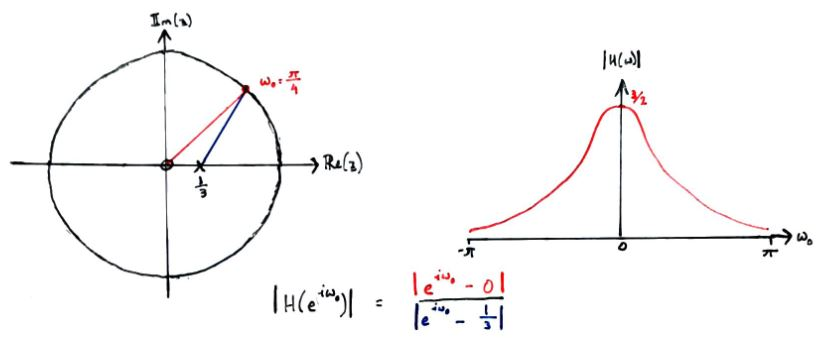
\includegraphics[width=\textwidth]{images/lecture_9_poles_zeroes.JPG}
  \caption{
    The magnitude response can be inferred from the pole-zero plot by
    computing the value of the transfer function on the unit circle in the
    complex plane. The ratio of the distances from zeroes and poles gives
    the value of the magnitude response at a point.
  }
  \label{fig::lecture_9_poles_zeroes}
\end{figure}
%
\begin{exmp}
  Consider the signal
  %
  \begin{displaymath}
    x[n] = \left(\frac{5}{6}\right)^n\sin\left(\frac{n\pi}{3}\right)u[n] \,.
  \end{displaymath}
  %
  In the previous lecture, we derived the Z-transform of the more general function
  %
  \begin{displaymath}
    \mathscr{Z}(r^n\sin(\omega_0 n)u[n]) = \frac{z^{-1}r\sin(\omega_0)}{1 - 2z^{-1}r\cos(\omega_0) + z^{-2}r^2} \,.
  \end{displaymath}
  %
  Comparing factors, we have $r=5/6$ and $\omega_0=\frac{\pi}{3}$.
  We found that the ROC was $|z| > |r|$, with a zero at $z = 0$ and poles
  at $z = r\ex{\im\omega_0}$. This allows us to draw the pole-zero plot
  in Figure \ref{fig::lecture_9_poles_zeroes_example_1},
  from which we can sketch the form of the magnitude response.
  In this case, we see that the system looks like a crude low-pass filter.
  %
  \begin{figure}[!htb]
    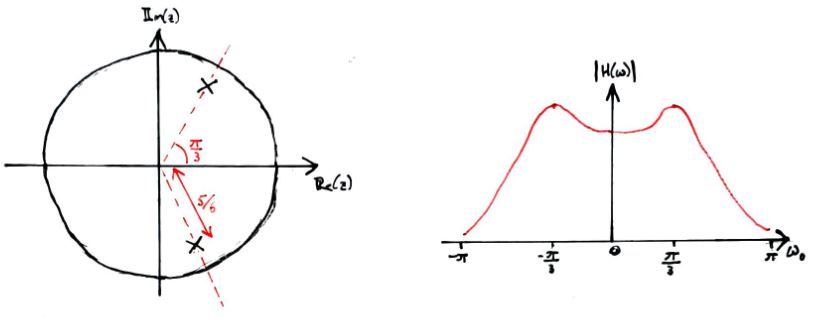
\includegraphics[width=\textwidth]{images/lecture_9_poles_zeroes_example_1.JPG}
    \caption{
      The pole-zero plot for the signal $x\left(\frac{5}{6}\right)^n\sin\left(\frac{n\pi}{3}\right)u[n]$
      and its corresponding magnitude response, which resembles a low-pass
      filter.
    }
    \label{fig::lecture_9_poles_zeroes_example_1}
  \end{figure}
  %
  Note that (somewhat unintuitively) shifting the poles inwards on the
  $\pm\frac{\pi}{3}$ lines in the complex plane has the effect of moving
  the local maxima that we see at the edges of the band-pass region of the
  filter. This is because the polynomials in the transfer function are products
  of all zeroes or poles -- the maxima in the magnitude response
  are not defined by the closest zero or pole, but some combination of all
  zeroes or poles.
\end{exmp}
%
Some further examples of converting pole-zero diagrams to magnitude responses
are given in Figures \ref{fig::lecture_9_poles_zeroes_example_2} and QQ.
%
\begin{figure}[!htb]
  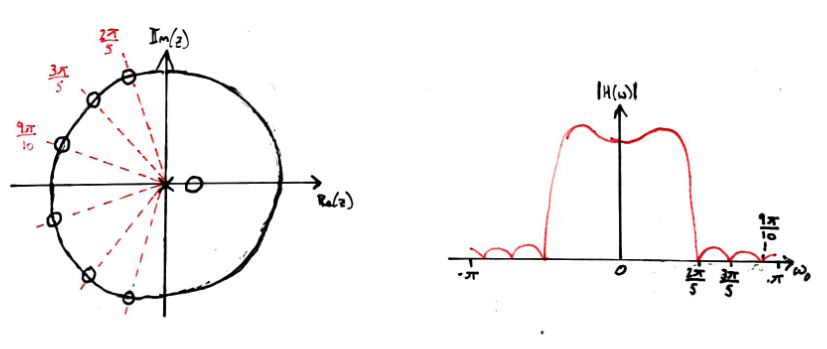
\includegraphics[width=\textwidth]{images/lecture_9_poles_zeroes_example_2.JPG}
  \caption{
    The pole-zero plot for a signal with poles at the origin in the complex plane
    and zeroes at $\omega = 0, \frac{2\pi}{5}, \frac{3\pi}{5}, \frac{9\pi}{10}$
    and its corresponding magnitude response, which resembles a low-pass filter..
  }
  \label{fig::lecture_9_poles_zeroes_example_2}
\end{figure}
%
What we've presented seems endlessly adaptable -- if we have a particular
filter characteristic we're looking to replicate, we can simply stick poles
and zeroes at pertinent places in the complex plane and we're done. In reality
however there are certain constraints on the locations of poles and zeroes
that we'll discuss in a later lecture. The number of poles and zeroes is also
constrained by the number of ``taps'' that are used for a filter, but this is
again something that will be discussed in due course.

\section{Lecture 10: The Discrete Fourier Transform}

\subsection{Introduction}
%
So far, we have identified that the Fourier Series can be used for
periodic, continuous-time systems. The Fourier Tranform is to be
used for aperiodic, continuous-time systems, while the Discrete
Time Fourier Transform is for aperiodic, discrete-time systems.
The final permutation that we're required to consider turns out
to be the most important for signal processing -- the
\textbf{Discrete Fourier Transform}, or DFT.

Recall that the Fourier Series takes a continuous, periodic
signal and represents it as a sum of (complex) sines and cosines,
%
\begin{displaymath}
  x(t) = \infsum{k} X[k]\ex{\im k\frac{2\pi}{T}t} \,,
\end{displaymath}
%
where $\frac{2\pi}{T} = \omega_0$, the fundamental frequency of the
signal, and $t$ is some continuous time variable taking a value
$0 \leq t \leq T$. Our rationale for the infinite summation was that
features such as discontinuities required infinitely many sinusoids
to recreate the structure of the function. In discrete time, however,
we can only have a finite number of discrete sinusoids by virtue of the
$2\pi$-periodicity of the DTFT. Simple substitution of a discrete-time
variable into the expression for the Fourier Series, i.e.
%
\begin{displaymath}
  x[n] = \infsum{k} X[k]\ex{\im k\frac{2\pi}{N}n} \,,
\end{displaymath}
%
doesn't make a great deal of sense since
%
\begin{displaymath}
  \ex{\im k\frac{2\pi}{N}(n + N)} = \ex{\im k\frac{2\pi}{N}n}\ex{\im k2\pi}
  = \ex{\im k \frac{2\pi}{N}n} \,,
\end{displaymath}
%
i.e. there are only $N$ unique complex exponentials of period $N$. This
makes sense from the perspective of linear algebra -- a mismatch in the
number of output values and the number of basis functions (the complex
exponentials in our case) leaves the system under- or over-determined,
and there is no longer any unique solution.

\subsection{The DFT Matrix}
%
Define the DFT as
%
\begin{equation}
  X[k] = \sum_{n=0}^{N-1}x[n]\ex{-\im k\frac{2\pi}{N}n},
  \quad k = 0,1,\hdots, N-1 \,,
\end{equation}
%
and its inverse, the IDFT,
%
\begin{equation}
  x[n] = \frac{1}{N}\sum_{k=0}^{N-1}X[k]\ex{\im k\frac{2\pi}{N}n},
  \quad n = 0,1,\hdots, N-1 \,.
\end{equation}
%
We can simplify this notation by introducing
$W_N=\ex{-\im\frac{2\pi}{N}}$, i.e. a point on the unit circle in the
complex plane whose angle is given by $\frac{2\pi}{N}$. $W_N$ is referred
to as an $N\th$ root of unity, since $(W_N)^N = 1$.
Taking $(W_N)^k$ increments its angle around the unit circle by $k$
units of $\frac{2\pi}{N}$. We can now rewrite the DFT,
%
\begin{equation}
  X[k] = \sum_{n=0}^{N-1}x[n]W_N^{kn} \,,
\end{equation}
%
and the IDFT as
%
\begin{equation}
  x[n] = \frac{1}{N}\sum_{k=0}^{N-1}X[k]W_N^{-kn} \,.
\end{equation}
%
From the theory of linear transformations, we see that the DFT can be
written in terms of matrix algebra,
%
\begin{displaymath}
  \vec{X}
  =
  \left[\begin{array}{cccc}
      W_N^{0,0} & W_N^{0,1} & \hdots & W_N^{0,N-1} \\
      W_N^{1,0} & W_N^{1,1} & \hdots & W_N^{1,N-1} \\
      \vdots & \vdots & \ddots & \vdots \\
      W_N^{N-1,0} & W_N^{N-1,1} & \hdots & W_N^{N-1,N-1}
  \end{array}\right]
  \left[\begin{array}{c}
      x_0 \\ x_1 \\ \vdots \\ x_{N-1}
  \end{array}\right]
  = \matr{W}\vec{x} \,,
\end{displaymath}
%
where $\matr{W}\in\mathbb{C}^{N\times N}$, and is referred to as the
\textbf{DFT matrix}. $\vec{x}$ and $\vec{X}$ are,
generally speaking, vectors in $\mathbb{C}^N$, although under certain conditions
can be real-valued. Note that;
%
\begin{itemize}
\item $\matr{W}$ is, by virtue of the orthogonality of
  the complex exponentials, unitary (the factor of $\frac{1}{N}$ in the
  IDFT preserves this unitarity, which satisfies Parseval's theorem, i.e. that
  the energy in both time and frequency domains remains the same). Herein we'll omit the
  subscript on the DFT matrix $\matr{W}$ since its size is implied by the lengths of $\vec{x}$
  and $\vec{X}$.
\item The DFT matrix has a special structure, where its first row and column
  contain $W^0$ only, which is one. This type of matrix is referred to as
  a Vandermonde matrix.
  
\end{itemize}
%
The matrix formulation gives us a little insight as to what's actually happening with
the DFT. Consider the value of $X[0]$, which is the inner product of the first row of
$\mathbf{W}$ and the vector $\mathbf{x}$. The first row of $\mathbf{W}$ is simply
a vector of ones, and so $X[0]$ is nothing more than the sum of elements of the
sampled signal, $\mathbf{x}$. Now, take the value of $X[1]$, which is the inner
product of the second row of $\mathbf{W}$ and the vector $\mathbf{x}$. This second
row of $\mathbf{W}$ samples each of the $N\th$ roots of unity, so that $x[k]$ is
multiplied by $W^k$. For $X[2]$, the elements in the third row of $\mathbf{W}$
sample every other root of unity; $W^0, W^2, W^4, \hdots$, wrapping around
the unit circle such that $W^N = W^0$. The pattern is then clear; for $X[k]$,
the input signal is modulated by the $N\th$ roots of unity, starting from $W^0$
and incrementing by an angle of $2\pi k/N$, accommodating the $2\pi$-periodicity.\\

Consider a finite-length discrete-time signal,
$\vec{x} = \left[\begin{array}{cccc}x[0] & x[1] & \hdots & x[N-1]\end{array}\right]^\top$.
The DTFT of this signal is
%
\begin{displaymath}
  X(\omega) = \infsum{n}x[n]\ex{-\im\omega n}, \quad \omega\in[-\pi,\pi] \,,
\end{displaymath}
%
i.e. a continuous function of $\omega$ which is $2\pi$-periodic. Since $\vec{x}$ is
only non-zero on the range $[0,N-1]$,
%
\begin{displaymath}
  X(\omega) = \sum_{n=0}^{N-1}x[n]\ex{-\im\omega n} \,.
\end{displaymath}
%
Looking at the form of the DFT, we see that the DFT is the DTFT evaluated at
$\omega_k = 2\pi k/N$,
%
\begin{displaymath}
  X[k] = X\left(\frac{2\pi k}{N}\right), \quad k = 0, 1, \hdots N-1 \,.
\end{displaymath}
%
In other words, the frequency response that we obtain via the DFT is the frequency
response obtained by the DTFT, but sampled at the points $2\pi k / N$ on the
$\omega$ axis. As $N\rightarrow\infty$, we recover the DTFT as the samples are separated
by an infinitesimal in $\omega$.
%
\begin{exmp}
  Consider the periodic discrete-time signal
  %
  \begin{displaymath}
    x[n + N] = \left\{\begin{array}{ccl}
      1 & & n = 0 \\
      0 & & \mathrm{otherwise}
    \end{array}\right. \,,
  \end{displaymath}
  i.e. the periodic delta function. From the DFT, we have
  %
  \begin{displaymath}
    X[k] = \sum_{n=0}^{N-1}x[n] W^{nk} = x[0]W^0 = 1 \,,
  \end{displaymath}
  %
  for all discrete frequencies $k$, as expected. Conversely, inverting this
  function with $X[k] = 1$,
  %
  \begin{displaymath}
    x[n] = \frac{1}{N}\sum_{k=0}^{N-1}X[k] W^{-nk}
    = \frac{1}{N}\sum_{k=0}^{N-1}W^{-nk} \,.
  \end{displaymath}
  %
  $x[0]$ is trivial to evaluate since it's equal to a sum of $W^0 = 1$,
  and our factor of $1/N$ then yields $x[0] = 1$. For $n\neq 0$, we need to
  invoke the finite sum formula,
  %
  \begin{displaymath}
    x[n] = \frac{1}{N}\sum_{k=0}^{N-1}W^{-nk}
    = \frac{1}{N}\frac{1-\left(W^{-n}\right)^{(N-1)+1}}{1 - W^{-n}}
    = \frac{1}{N}\frac{1-W^{-nN}}{1 - W^{-n}} \quad n\neq 0 \,.
  \end{displaymath}
  %
  Note that $W$ to some integer multiple of $N$ corresponds to nothing more
  than $N$ complete rotations around the complex plane, always yielding $1$,
  and consequently
  %
  \begin{displaymath}
    x[0] = \frac{1}{N}\frac{1-W^{-nN}}{1 - W^{-n}}
    = \frac{1}{N}\frac{1-W^0}{1 - W^{-n}}
    = \frac{1}{N}\frac{0}{1 - W^{-n}} = 0 \quad n\neq 0 \,.
  \end{displaymath}
  In other words, we've recovered the delta function, and we've established
  the duality of the time-domain signal and the DFT.
\end{exmp}
%
The above example uses a key property of the Fourier matrix, referred to
as the \textbf{orthogonality property}, which we'll invoke frequently
throughout the remaining discussion:
%
\begin{equation}
  \sum_{n=0}^{N-1}W_N^{mn} = \left\{\begin{array}{ccl}
    N & & m\;\mathrm{mod}\;N = 0 \\
    0 & & \mathrm{otherwise} 
  \end{array}\right. \,.
\end{equation}
%
\begin{exmp}
  Consider the top-hat signal
  %
  \begin{displaymath}
    x[n] =
    \left\{\begin{array}{ccl}
    1 & & 0 \leq n < 5 \\
    0 & & \mathrm{otherwise}
    \end{array}\right. \,.
  \end{displaymath}
  %
  By the finite sum formula, the DTFT of this signal is
  %
  \begin{displaymath}
    X(\omega) = \infsum{n}x[n]\ex{-\im\omega n}
    = \sum_{n=0}^4\ex{-\im\omega n}
    = \frac{1 - \ex{-5\im\omega}}{1 - \ex{-\im\omega}} \,.
  \end{displaymath}
  %
  Factoring out an exponential in both numerator and denominator,
  %
  \begin{displaymath}
    X(\omega) = \frac{
      \ex{-5\im\omega/2}\left(\ex{5\im\omega/2} - \ex{-5\im\omega/2}\right)
    }{
      \ex{-\im\omega/2}\left(\ex{\im\omega/2} - \ex{-\im\omega/2}\right)
    } = \ex{-2\im\omega}\frac{
      \sin\left(5\omega/2\right)
    }{
      \sin\left(\omega/2\right)
    } \,.
  \end{displaymath}
  %
  Now let's try to treat this as a length-10 discrete-time signal,
  %
  \begin{displaymath}
    X[k] = \sum_{n=0}^9 x[n]W_{10}^{kn} = \sum_{n=0}^4 W_{10}^{kn}
    = \frac{1 - W_{10}^{5k}}{1 - W_{10}}
    = \frac{1 - \ex{-\pi\im k}}{1 - \ex{-\pi\im k/5}} \,,
  \end{displaymath}
  %
  and doing the same manipulation as before,
  %
  \begin{displaymath}
    X[k] = \frac{
      \ex{-\pi\im k/2}(\ex{\pi\im k/2} - \ex{-\pi\im k/2}) 
    }{
      \ex{-\pi\im k/10}(\ex{\pi\im k/10} - \ex{-\pi\im k/10}) 
    } = \ex{-2\pi\im k / 5} \frac{
      \sin\left(\pi k/2\right)
    }{
      \sin\left(\pi k/10\right)
    } \,.
  \end{displaymath}
  %
  Recalling that the DFT is just the DTFT sampled at the points
  $\omega = 2\pi k/N$, we see that
  %
  \begin{displaymath}
    X(\omega) = \ex{-2\im\omega}\frac{
      \sin\left(5\omega/2\right)
    }{
      \sin\left(\omega/2\right)
    } =
    \ex{-2\pi\im k / 5}\frac{
      \sin\left(\pi k/2\right)
    }{
      \sin\left(\pi k/10\right)
    } = X[k] \,,
  \end{displaymath}
  %
  as required.
\end{exmp}

\subsection{Properties of the DFT}
%
\begin{enumerate}
\item (\textbf{Linearity}) Given the signals $x_1[n]$ and $x_2[n]$, each
  of period $N$,
  %
  \begin{displaymath}
    ax_1[n] + bx_2[n] \Longleftrightarrow aX_1[k] + bX_2[k] \,. 
  \end{displaymath}
  %
\item (\textbf{Symmetry}) If $x[n]$ is even, then $X[k]$ is real and even.
  Conversely, if $x[n]$ is odd, then $X[k]$ is imaginary and odd.
  %
\item (\textbf{Time-Shifting}) For the time-shifted signal,
  %
  \begin{displaymath}
    x[n-m] \Longleftrightarrow W_N^{km}X[k] \,.
  \end{displaymath}
  %
  Note that shifting a periodic signal is a cyclic shift.
  %
\item (\textbf{Convolution}) For the signals $x[n] \Longleftrightarrow X[k]$
  and $y[n] \Longleftrightarrow Y[k]$, which are both $N$-periodic,
  %
  \begin{displaymath}
    x[n]y[n] \Longleftrightarrow X[k]\circledast Y[k] \,,
  \end{displaymath}
  %
  where $\circledast$ denotes the cyclic convolution. 
\end{enumerate}

\subsection{Making Sense Of Discrete Frequencies}
%
For the Fourier Transform, we expect the spectrum to consist of both positive
and negative frequencies. However, with the DFT we've simply acquired a list
of frequencies indexed from $0$ to $N-1$; so where have the negative
frequency components ended up? Let's consider the case where $N$ is even. Then,
%
\begin{displaymath}
  X[N/2] = \sum_{k=0}^{N-1}x[k]W^{kN/2} = \sum_{k=0}^{N-1}x[k]\ex{-\im\pi k}
  = \sum_{k=0}^{N-1}(-1)^k x[k] \,,
\end{displaymath}
%
which is strictly real-valued for a real signal; it's just the sum of elements of
the signal, where each element is multiplied by either $\pm 1$. Now consider the
frequencies on either side of $x[N/2]$:
%
\begin{align*}
  X\left[\frac{N}{2}+1\right] &= \sum_{k=0}^{N-1}x[k]W^{k\left(\frac{N}{2}+1\right)}
  = \sum_{k=0}^{N-1}x[k]W^{kN/2}W^{k} = \sum_{k=0}^{N-1}x[k](-1)^{k}W^{k} \\
  X\left[\frac{N}{2}-1\right] &= \sum_{k=0}^{N-1}x[k]W^{k\left(\frac{N}{2}-1\right)}
  = \sum_{k=0}^{N-1}x[k]W^{kN/2}W^{-k} = \sum_{k=0}^{N-1}x[k](-1)^{k} W^{-k} \,,
\end{align*}
%
which are equal with the exception of the factor of $W^{\pm k}$. These two expressions
are no more than the complex conjugates of one another,
%
\begin{displaymath}
  X\left[\frac{N}{2}+1\right] = X\left[\frac{N}{2}-1\right]^* \,,
\end{displaymath}
%
and this pattern persists for any $m = 1,\hdots,\frac{N}{2}-1$,
%
\begin{displaymath}
  X\left[\frac{N}{2}+m\right] = X\left[\frac{N}{2}-m\right]^* \,.
\end{displaymath}
%
From what we know about the Hermitian symmetry of the Fourier Transform, this
means that $X[N/2]$ must correspond to the central frequency in the DTFT,
$X(0)$; the fact that this value always satisfies the Hermitian symmetry
requiring this element be its own complex conjugate. Furthermore, the DC
component corresponds to $X[0]$ since
%
\begin{displaymath}
  X[0] = \sum_{k=0}^{N-1}x[k] W^{k\times 0} = \sum_{k=0}^{N-1}x[k] \,,
\end{displaymath}
%
the sum of the input signal values. The components $X[1], X[2], \hdots, X[N/2]$
then form the series of increasing frequencies, with $X[N/2]$ being the
Nyquist frequency (see later lecture); an alternating sum of signal components.\\

We might also query to what \textit{actual} frequencies do these discretised
frequencies correspond? We know that $N$ samples in the time domain become
$N$ samples in the frequency domain. A signal duration $L$ maps to a frequency
spectrum of width $2B$, where $B$ is the bandwidth of the signal (the factor
of 2 comes from the fact that we have both positive and negative frequencies).
From the reciprocity of time and frequency, we know that in the time-domain,
$L/N = 1/2B$, the interval between samples. Similarly, in the frequency-domain,
$2B/N = 1/L$, the interval between discrete frequencies. These two conditions
present us with the same \textbf{reciprocity relation},
%
\begin{displaymath}
  2BL = N \,.
\end{displaymath}
%
So, for instance, if we have a signal of duration $L=1\mathrm{ms}$ and its
sampled with $1024$ points, the bandwidth of the signal captured by the
DFT is $1024 / 2\times 10^{-3} = 512\mathrm{kHz}$, and the discrete frequencies
$X[k]$ are separated by
$1/10^{-3}\mathrm{secs} = 2\times 512\mathrm{kHz} / 1024 = 1\mathrm{kHz}$.

\subsection{Discrete-Time Convolution}
%
The duality between cyclic convolution and multiplication in the time/ frequency
domains poses something of a problem for our treatment of LTI systems, where
the output of an LTI system is given by the ``regular'' convolution of an
input signal and the system's impulse response. Let's explicitly consider what
is happening with the cyclic convolution with some examples. Let $x[n]$ and $h[n]$
be length-5 periodic signals. Then,
%
\begin{displaymath}
  x[n]\circledast h[n] =
  \left[\begin{array}{c}
      y_0 \\ y_1 \\ y_2 \\ y_3 \\ y_4
    \end{array}\right] =
  \left[\begin{array}{c}
      h_0x_0 + h_4x_1 + h_3x_2 + h_2x_3 + h_1x_4 \\
      h_1x_0 + h_0x_1 + h_4x_2 + h_3x_3 + h_2x_4 \\
      h_2x_0 + h_1x_1 + h_0x_2 + h_4x_3 + h_3x_4 \\
      h_3x_0 + h_2x_1 + h_1x_2 + h_0x_3 + h_4x_4 \\
      h_4x_0 + h_3x_1 + h_2x_2 + h_1x_3 + h_0x_4
    \end{array}\right]
  = \left[\begin{array}{ccccc}
      \red{h_0} & \orn{h_4} & \yel{h_3} & \grn{h_2} & \blu{h_1} \\
      \blu{h_1} & \red{h_0} & \orn{h_4} & \yel{h_3} & \grn{h_2} \\
      \grn{h_2} & \blu{h_1} & \red{h_0} & \orn{h_4} & \yel{h_3} \\
      \yel{h_3} & \grn{h_2} & \blu{h_1} & \red{h_0} & \orn{h_4} \\
      \orn{h_4} & \yel{h_3} & \grn{h_2} & \blu{h_1} & \red{h_0}
    \end{array}\right] \left[\begin{array}{c}
      x_0 \\ x_1 \\ x_2 \\ x_3 \\ x_4
    \end{array}\right] \,,
\end{displaymath}
%
where we have noticed that the summation of elements of $x[n]$ and $h[n]$
resembles a linear transformation of the $x[n]$ by $h[n]$ when placed into
the matrix in the final expression. This matrix has a particular form which
is emphasised by our choice of colour -- it is referred to as a \textbf{circulant}
matrix.\\
%
Now, consider what is happening with the ``regular'' linear convolution when we
try to represent it as a linear transformation of the $x[n]$,
%
\begin{displaymath}
  x[n] * h[n] =
  \left[\begin{array}{c}
      y_0 \\ y_1 \\ y_2 \\ y_3 \\ y_4 \\ y_5 \\ y_6 \\ y_7 \\ y_8
    \end{array}\right] =
  \left[\begin{array}{l}
      h_0x_0 \\
      h_1x_0 + h_0x_1 \\
      h_2x_0 + h_1x_1 + h_0x_2 \\
      h_3x_0 + h_2x_1 + h_1x_2 + h_0x_3 \\
      h_4x_0 + h_3x_1 + h_2x_2 + h_1x_3 + h_0x_4 \\
      h_4x_1 + h_3x_2 + h_2x_3 + h_1x_4 \\
      h_4x_2 + h_3x_3 + h_2x_4 \\
      h_4x_3 + h_3x_4 \\
      h_4x_4
    \end{array}\right]
  = \left[\begin{array}{ccccc}
      \red{h_0} & 0 & 0 & 0 & 0 \\
      \blu{h_1} & \red{h_0} & 0 & 0 & 0 \\
      \grn{h_2} & \blu{h_1} & \red{h_0} & 0 & 0 \\
      \yel{h_3} & \grn{h_2} & \blu{h_1} & \red{h_0} & 0 \\
      \orn{h_4} & \yel{h_3} & \grn{h_2} & \blu{h_1} & \red{h_0} \\
      0 & \orn{h_4} & \yel{h_3} & \grn{h_2} & \blu{h_1} \\
      0 & 0 & \orn{h_4} & \yel{h_3} & \grn{h_2} \\
      0 & 0 & 0 & \orn{h_4} & \yel{h_3} \\
      0 & 0 & 0 & 0 &\orn{h_4}
    \end{array}\right] \left[\begin{array}{c}
      x_0 \\ x_1 \\ x_2 \\ x_3 \\ x_4
    \end{array}\right] \,,
\end{displaymath}
%
where we have to accommodate the prologue and epilogue phases of
the convolution, i.e. when $h[n]$ doesn't fully overlap with $x[n]$
during the ``flip and slide''.\\
%
Our solution to recovering the linear convolution from a cyclic
convolution is to use \textbf{zero-padding}. Generally speaking, consider
$h[n]$ is length $N$ and $x[m]$ is length $M$. Then, by padding $h[n]$
with $M-1$ zeroes at the end of the signal, and by padding $x[m]$ with
$N-1$ zeroes at the end of the signal, so that both are length $N+M-1$,
and referring to these padded signals as $h_p[n]$ and $x_p[m]$, respectively,
%
\begin{displaymath}
  x_p[m] * h_p[n] =
  \left[\begin{array}{c}
      y_0 \\ y_1 \\ y_2 \\ y_3 \\ y_4 \\ y_5 \\ y_6 \\ y_7 \\ y_8
    \end{array}\right]
  = \left[\begin{array}{ccccccccc}
      \red{h_0} & 0 & 0 & 0 & 0 & \blu{h_4} & \grn{h_3} & \yel{h_2} & \orn{h_1} \\
      \blu{h_1} & \red{h_0} & 0 & 0 & 0 & 0 & \blu{h_4} & \grn{h_3} & \yel{h_2} \\
      \grn{h_2} & \blu{h_1} & \red{h_0} & 0 & 0 & 0 & 0 & \blu{h_4} & \grn{h_3} \\
      \yel{h_3} & \grn{h_2} & \blu{h_1} & \red{h_0} & 0 & 0 & 0 & 0 & \blu{h_4} \\
      \orn{h_4} & \yel{h_3} & \grn{h_2} & \blu{h_1} & \red{h_0} & 0 & 0 & 0 & 0 \\
      0 & \orn{h_4} & \yel{h_3} & \grn{h_2} & \blu{h_1} & \red{h_0} & 0 & 0 & 0 \\
      0 & 0 & \orn{h_4} & \yel{h_3} & \grn{h_2} & \blu{h_1} & \red{h_0} & 0 & 0 \\
      0 & 0 & 0 & \orn{h_4} & \yel{h_3} & \grn{h_2} & \blu{h_1} & \red{h_0} & 0 \\
      0 & 0 & 0 & 0 & \orn{h_4} & \yel{h_3} & \grn{h_2} & \blu{h_1} & \red{h_0}
    \end{array}\right] \left[\begin{array}{c}
      x_0 \\ x_1 \\ x_2 \\ x_3 \\ x_4 \\ 0 \\ 0 \\ 0 \\ 0
    \end{array}\right] \,,
\end{displaymath}
%
which recovers the result of the linear convolution. Our conclusion is then to do linear
convolution with the DFT, we must first zero-pad our two signals, perform
DFTs of both, multiply these two signals in the frequency domain and finally
perform an IDFT to recover the linear convolution in the time domain.


\section{Lecture 11: The Radix-2 Fast Fourier Transform}

Consider the DFT,
%
\begin{displaymath}
  X[k] = \sum_{n=0}^{N-1}x[n]\ex{-\im k\frac{2\pi}{N}n},\quad
  n,k = 0, 1, \hdots N-1 \,,
\end{displaymath}
%
which in abbreviated form becomes
%
\begin{displaymath}
  X[k] = \sum_{n=0}^{N-1}x[n]W_N^{kn} \,,
\end{displaymath}
%
with $W_N = \ex{-\im\frac{2\pi}{N}}$, and $W_N^m$ for $m=1,2,\hdots,N$
are the $n$\textsuperscript{th} roots of unity, which are evenly spaced
around the unit circle on the complex plane. Analysing the computational
complexity of this, to compute the $\{X[k]\}$, we need to compute $N^2$
complex multiplications and $N(N-1)$ complex additions (assuming the
$W_N^m$ are pre-calculated). Quadratic scaling in the problem complexity
is not tractable for large $N$, and consequently much work has been
conducted to find a more efficient way to compute the DFT.\\

The \textbf{Fast Fourier Transform} (FFT) is an algorithm which reduces
the number of operations to $\mathcal{O}(N\log N)$. The main tool we'll
use to achieve this is the decomposition of a large DFT into a series of
smaller DFTs. Furthermore, there are some simplifications we can apply
to the $W_N^{km}$ to simplify the calculation.

\subsection{Decimation in Time}
%
Consider $N$ as an even number. We can break the expression for the DFT
into separate sums over odd- and even-valued indices,
%
\begin{displaymath}
  X[k] = \sum_{n=0}^{N-1}x[n]W_N^{nk}
  = \sum_{n \mathrm{Even}}x[n] W_N^{nk}
  + \sum_{n \mathrm{Odd}}x[n] W_N^{nk} \,.
\end{displaymath}
%
Introducing a new index, $r$, such that $n=2r$,
%
\begin{align*}
  X[k] &= \sum_{r=0}^{N/2-1} x[2r] W_N^{2rk}
  + \sum_{r=0}^{N/2-1} x[2r+1] W_N^{(2r+1)k} \\
  &= \sum_{r=0}^{N/2-1}x[2r]\left(W_N^2\right)^{rk}
  + W_N^k\sum_{r=0}^{N/2-1}x[2r+1]\left(W_N^2\right)^{rk} \,,
\end{align*}
%
where each sum looks suspiciously like a DFT of length $N/2$. Indeed,
it transpires that each of these sums is precisely a length $N/2$ DFT,
since $W_N^2$ are the $N/2$ roots of unity. For example, consider
$W_4 = \{ \ex{-\im\frac{2\pi}{4}}, \ex{-\im\frac{4\pi}{4}}, \ex{-\im\frac{6\pi}{4}}, \ex{-\im\frac{8\pi}{4}} \}$,
the fourth roots of unity. Then,
$W_4^2 = \{ \ex{-\im\frac{4\pi}{4}}, \ex{-\im\frac{8\pi}{4}} \}$, the
second roots of unity, i.e. $W_2$. Consequently,
%
\begin{displaymath}
  X[k] = 
  \sum_{r=0}^{N/2-1}x[2r] W_{N/2}^{rk}
  + W_N^k\sum_{r=0}^{N/2-1}x[2r+1] W_{N/2}^{rk}
  = X_e[k] + W_N^k X_o[k] \,,
\end{displaymath}
%
where $X_e[k]$ is the DFT of the even-indexed elements of $x[n]$,
and $X_o[k]$ is the DFT of the odd-indexed elements of $x[n]$. The
computational process behind computing the $X[k]$ using this partition
into even and odd DFTs is shown in Figure \ref{fig::lecture_11_dft_one}.
%
\begin{figure}[H]
  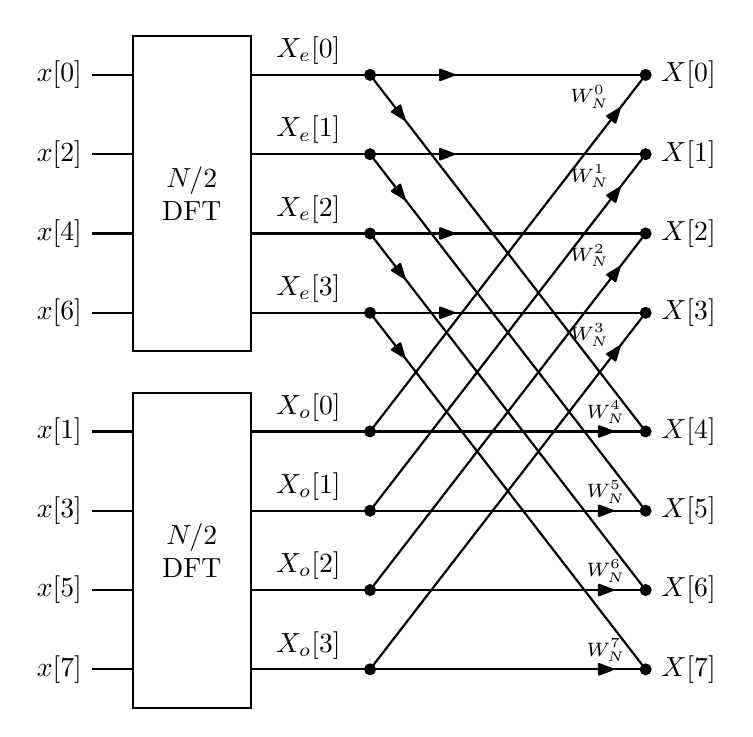
\begin{tikzpicture}[
    thick, node distance=.5cm, circuit ee IEC,
    box/.style={
      draw, align=center, shape=rectangle, minimum width=1.5cm, minimum height=4cm,
      append after command={% see also: https://tex.stackexchange.com/a/129668
        \foreach \side in {east,west} {
          \foreach \i in {1,...,#1} {
            %          coordinate (\tikzlastnode-\i-\side)
            %          at ($(\tikzlastnode.north \side)!{(\i-.5)/(#1)}!(\tikzlastnode.south \side)$)
            (\tikzlastnode.north \side) edge[draw=none, line to]
            coordinate[pos=(\i-.5)/(#1)] (\tikzlastnode-\i-\side) (\tikzlastnode.south \side)
  }}}}]
  \node[box=4] (box-t) {$N/2$ \\ DFT};
  \node[box=4, below=of box-t] (box-b) {$N/2$ \\ DFT};

  \foreach \s[count=\i] in {0,2,4,6}
  \path (box-t-\i-west) edge node[at end, left]{$x[\s]$} ++(left:.5);
  \foreach \s[count=\i] in {1,3,5,7}
  \path (box-b-\i-west) edge node[at end, left]{$x[\s]$} ++(left:.5);

  \foreach \b/\s[count=\k] in {t/e, b/o}
  \foreach \i[evaluate={\j=int(\i-1)},
    evaluate={\J=int(ifthenelse(\k==2,\j+4,\j))}] in {1,...,4}
  \node [contact] (conn-\b-\i) at ([shift=(right:1.5)] box-\b-\i-east) {}
  edge node[above] {$X_{\s}[\j]$} (box-\b-\i-east)
  node [contact, label=right:{$X[\J]$}] (conn-\b-\i') at ([shift=(right:5)] box-\b-\i-east) {};

  \begin{scope}[every info/.append style={font=\scriptsize, inner sep=+.5pt}]

    \foreach \i[evaluate={\j=int(\i-1)},evaluate={\J=int(\i+3)}] in {1,...,4}
    \path (conn-t-\i) edge[current direction={pos=.27}] (conn-t-\i')
    edge[current direction={pos=.1}] (conn-b-\i')
    (conn-b-\i) edge[current direction={pos=.87, info={$W_N^\J$}}] (conn-b-\i')
    edge[current direction={pos=.9, info={$W_N^\j$}}] (conn-t-\i');
  \end{scope}
\end{tikzpicture}

  \caption{DFT for a length-8 signal. DFTs of length $N/2$ are taken for the
    even and odd-indexed elements of $x[n]$ and recombined to compute the full
    DFT of the original signal.
  }
  \label{fig::lecture_11_dft_one}
\end{figure}
%
We know that the number of complex multiplications in a DFT scales like $N^2$.
Splitting our calculation into two DFTs of length $N/2$ then turns the
complexity into $N^2 / 2$, i.e. we've halved the computational effort associated
with the complex multiplications. Note that we also have to multiply by the
$\{W_N\}$ to recover the $X[k]$, but this operation is linear in $N$ and so
doesn't affect the complexity. It should not have escaped the reader's attention
that we can repeat this trick again on the DFTs for $X_e[n]$ and $X_o[n]$.
We'll require the even and odd parts of $X_e[n]$ ($X_{ee}[n]$ and $X_{eo}[n]$,
respectively) and $X_o[n]$ ($X_{oe}[n]$ and $X_{oo}[n]$, respectively).
This scheme is depicted in Figure \ref{fig::lecture_11_dft_two}.
%
\begin{figure}[H]
  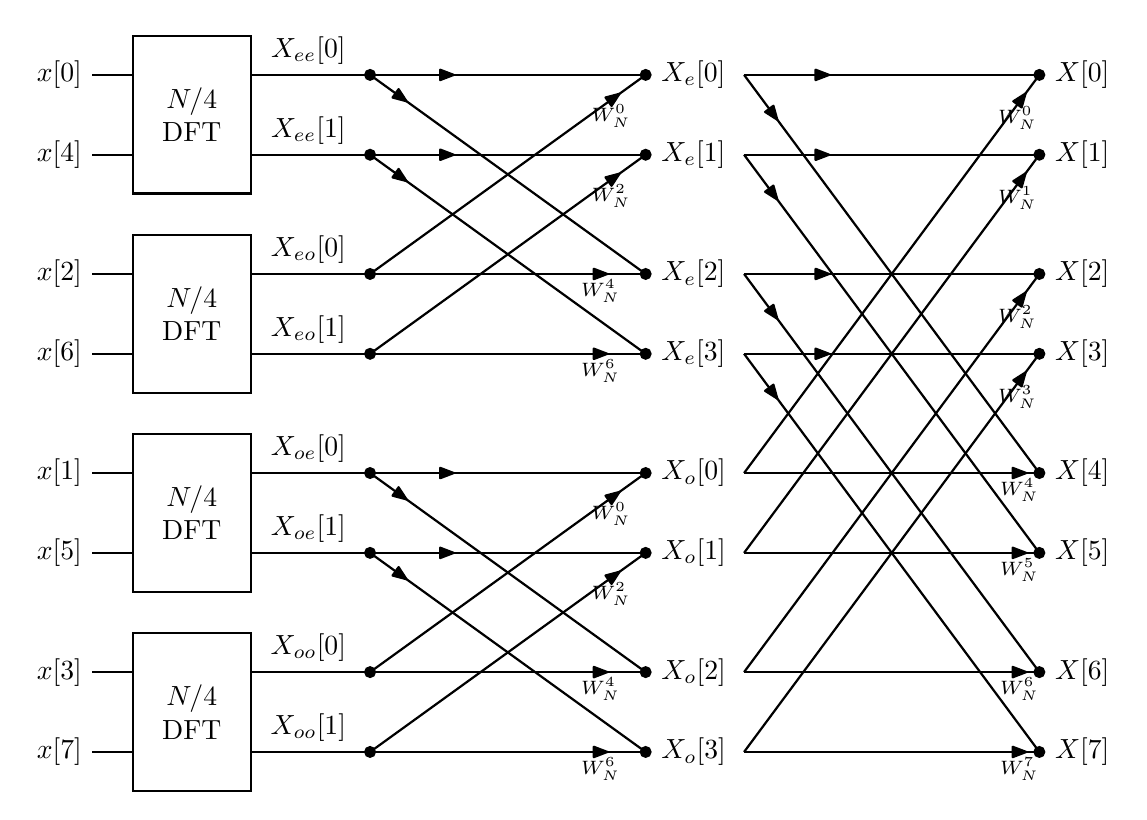
\begin{tikzpicture}[
  thick, node distance=.5cm, circuit ee IEC,
  box/.style={
    draw, align=center, shape=rectangle, minimum width=1.5cm, %minimum height=4cm,
    append after command={% see also: https://tex.stackexchange.com/a/129668
      \foreach \side in {east,west} {
        \foreach \i in {1,...,#1} {
          %          coordinate (\tikzlastnode-\i-\side)
          %          at ($(\tikzlastnode.north \side)!{(\i-.5)/(#1)}!(\tikzlastnode.south \side)$)
          (\tikzlastnode.north \side) edge[draw=none, line to]
          coordinate[pos=(\i-.5)/(#1)] (\tikzlastnode-\i-\side) (\tikzlastnode.south \side)
        }
      }
    }
  }
]


  \node[box=2, minimum height=2cm] (box-w) {$N/4$ \\ DFT};
  \node[box=2, below=of box-w, minimum height=2cm] (box-x) {$N/4$ \\ DFT};
  \node[box=2, below=of box-x, minimum height=2cm] (box-y) {$N/4$ \\ DFT};
  \node[box=2, below=of box-y, minimum height=2cm] (box-z) {$N/4$ \\ DFT};

  \foreach \s[count=\i] in {0,4}
  \path (box-w-\i-west) edge node[at end, left]{$x[\s]$} ++(left:.5);
  \foreach \s[count=\i] in {2,6}
  \path (box-x-\i-west) edge node[at end, left]{$x[\s]$} ++(left:.5);
  \foreach \s[count=\i] in {1,5}
  \path (box-y-\i-west) edge node[at end, left]{$x[\s]$} ++(left:.5);
  \foreach \s[count=\i] in {3,7}
  \path (box-z-\i-west) edge node[at end, left]{$x[\s]$} ++(left:.5);

  \node [contact] (conn-ee-0) at ([shift=(right:1.5)] box-w-1-east) {}
  edge node[above] {$X_{ee}[0]$} (box-w-1-east)
  node [contact, label=right:{$X_e[0]$}] (conn-e-0) at ([shift=(right:5)] box-w-1-east) {}
  node [contact, label=right:{$X[0]$}] (conn-0) at ([shift=(right:5)] conn-e-0) {};
  \node [contact] (conn-ee-1) at ([shift=(right:1.5)] box-w-2-east) {}
  edge node[above] {$X_{ee}[1]$} (box-w-2-east)
  node [contact, label=right:{$X_e[1]$}] (conn-e-1) at ([shift=(right:5)] box-w-2-east) {}
  node [contact, label=right:{$X[1]$}] (conn-1) at ([shift=(right:5)] conn-e-1) {};

  \node [contact] (conn-eo-0) at ([shift=(right:1.5)] box-x-1-east) {}
  edge node[above] {$X_{eo}[0]$} (box-x-1-east)
  node [contact, label=right:{$X_e[2]$}] (conn-e-2) at ([shift=(right:5)] box-x-1-east) {}
  node [contact, label=right:{$X[2]$}] (conn-2) at ([shift=(right:5)] conn-e-2) {};
  \node [contact] (conn-eo-1) at ([shift=(right:1.5)] box-x-2-east) {}
  edge node[above] {$X_{eo}[1]$} (box-x-2-east)
  node [contact, label=right:{$X_e[3]$}] (conn-e-3) at ([shift=(right:5)] box-x-2-east) {}
  node [contact, label=right:{$X[3]$}] (conn-3) at ([shift=(right:5)] conn-e-3) {};

  \node [contact] (conn-oe-0) at ([shift=(right:1.5)] box-y-1-east) {}
  edge node[above] {$X_{oe}[0]$} (box-y-1-east)
  node [contact, label=right:{$X_o[0]$}] (conn-o-0) at ([shift=(right:5)] box-y-1-east) {}
  node [contact, label=right:{$X[4]$}] (conn-4) at ([shift=(right:5)] conn-o-0) {};
  \node [contact] (conn-oe-1) at ([shift=(right:1.5)] box-y-2-east) {}
  edge node[above] {$X_{oe}[1]$} (box-y-2-east)
  node [contact, label=right:{$X_o[1]$}] (conn-o-1) at ([shift=(right:5)] box-y-2-east) {}
  node [contact, label=right:{$X[5]$}] (conn-5) at ([shift=(right:5)] conn-o-1) {};
  
  \node [contact] (conn-oo-0) at ([shift=(right:1.5)] box-z-1-east) {}
  edge node[above] {$X_{oo}[0]$} (box-z-1-east)
  node [contact, label=right:{$X_o[2]$}] (conn-o-2) at ([shift=(right:5)] box-z-1-east) {}
  node [contact, label=right:{$X[6]$}] (conn-6) at ([shift=(right:5)] conn-o-2) {};
  \node [contact] (conn-oo-1) at ([shift=(right:1.5)] box-z-2-east) {}
  edge node[above] {$X_{oo}[1]$} (box-z-2-east)
  node [contact, label=right:{$X_o[3]$}] (conn-o-3) at ([shift=(right:5)] box-z-2-east) {}
  node [contact, label=right:{$X[7]$}] (conn-7) at ([shift=(right:5)] conn-o-3) {};

  \begin{scope}[every info/.append style={font=\scriptsize, inner sep=+.5pt, below=3pt}]

    \path (conn-ee-0) edge[current direction={pos=.27}] (conn-e-0)
    edge[current direction={pos=.1}] (conn-e-2)
    (conn-eo-0) edge[current direction={pos=.9, info={$W_N^0$}}] (conn-e-0)
    edge[current direction={pos=.85, info={$W_N^4$}}] (conn-e-2);

    \path (conn-ee-1) edge[current direction={pos=.27}] (conn-e-1)
    edge[current direction={pos=.1}] (conn-e-3)
    (conn-eo-1) edge[current direction={pos=.9, info={$W_N^2$}}] (conn-e-1)
    edge[current direction={pos=.85, info={$W_N^6$}}] (conn-e-3);

    \path (conn-oe-0) edge[current direction={pos=.27}] (conn-o-0)
    edge[current direction={pos=.1}] (conn-o-2)
    (conn-oo-0) edge[current direction={pos=.9, info={$W_N^0$}}] (conn-o-0)
    edge[current direction={pos=.85, info={$W_N^4$}}] (conn-o-2);

    \path (conn-oe-1) edge[current direction={pos=.27}] (conn-o-1)
    edge[current direction={pos=.1}] (conn-o-3)
    (conn-oo-1) edge[current direction={pos=.9, info={$W_N^2$}}] (conn-o-1)
    edge[current direction={pos=.85, info={$W_N^6$}}] (conn-o-3);

    

    \path (conn-e-0) ++(1.25,0) edge[current direction={pos=.27}] (conn-0)
    edge[current direction={pos=.1}] (conn-4)
    (conn-o-0) ++(1.25,0) edge[current direction={pos=.95, info={$W_N^0$}}] (conn-0)
    edge[current direction={pos=.95, info={$W_N^4$}}] (conn-4);

    \path (conn-e-1) ++(1.25,0) edge[current direction={pos=.27}] (conn-1)
    edge[current direction={pos=.1}] (conn-5)
    (conn-o-1) ++(1.25,0) edge[current direction={pos=.95, info={$W_N^1$}}] (conn-1)
    edge[current direction={pos=.95, info={$W_N^5$}}] (conn-5);

    \path (conn-e-2) ++(1.25,0) edge[current direction={pos=.27}] (conn-2)
    edge[current direction={pos=.1}] (conn-6)
    (conn-o-2) ++(1.25,0) edge[current direction={pos=.95, info={$W_N^2$}}] (conn-2)
    edge[current direction={pos=.95, info={$W_N^6$}}] (conn-6);

    \path (conn-e-3) ++(1.25,0) edge[current direction={pos=.27}] (conn-3)
    edge[current direction={pos=.1}] (conn-7)
    (conn-o-3) ++(1.25,0) edge[current direction={pos=.95, info={$W_N^3$}}] (conn-3)
    edge[current direction={pos=.95, info={$W_N^7$}}] (conn-7);    
    
  \end{scope}

  
\end{tikzpicture}

  \caption{DFT for a length-8 signal using length-2 DFTs. DFTs of length $N/4$
    are taken for the even-even, even-odd, odd-even and odd-even indexed elements
    of $x[n]$ and recombined to compute the full DFT of the original signal.
  }
  \label{fig::lecture_11_dft_two}
\end{figure}
%
The computational complexity of this DFT is $N^2 / 4$ in the number of complex
multiplications, and so we've halved the computational effort again. In fact,
our efficiency is improved further when considering the form of a length-2 DFT:
%
\begin{displaymath}
  X[k] = \sum_{n=0}^1 x[n]W_2^{nk} = \sum_{n=0}^1 x[n](-1)^{nk} \,,
\end{displaymath}
%
since the second roots of unity are simply $1,-1$, and so
%
\begin{displaymath}
  X[0] = x[0] + x[1],\quad X[1] = x[0] - x[1] \,,
\end{displaymath}
%
which contains no complex multiplications whatsoever! The scheme becomes
like that depicted in Figure \ref{fig::lecture_11_dft_three}. The operation
of combining two values to yield two different values (the cross-shaped patterns
in the DFT figures) are referred to as \textbf{butterflies}.  
%
\begin{figure}[H]
  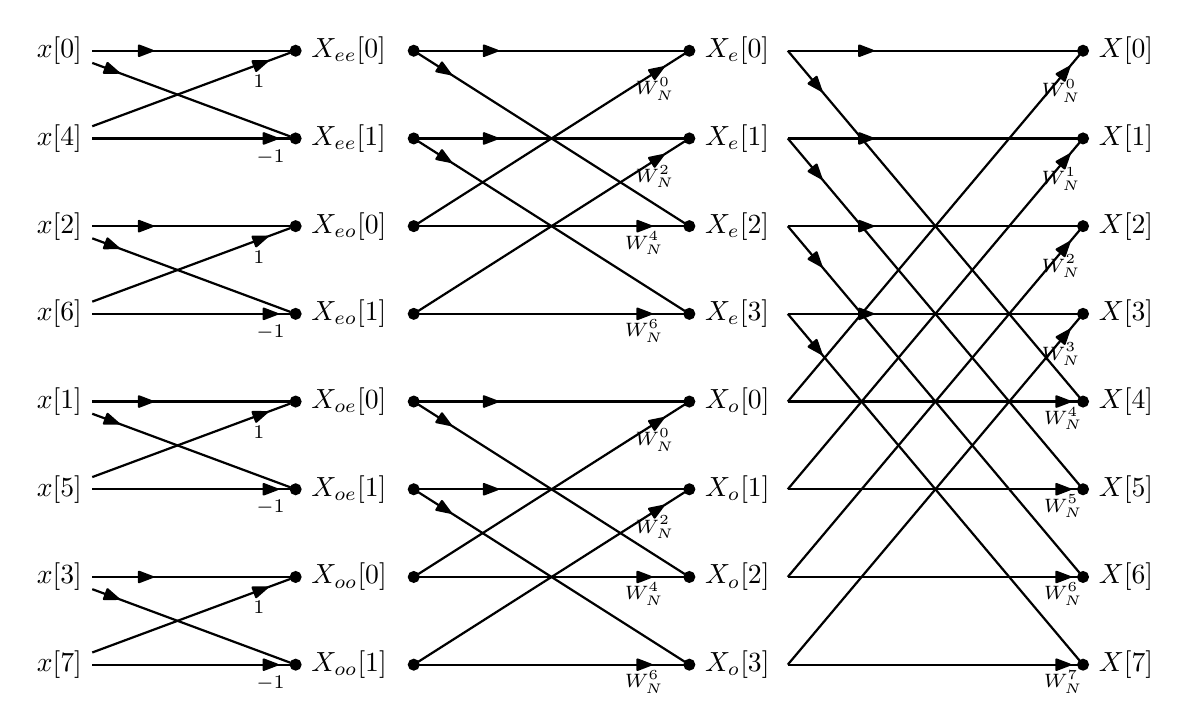
\begin{tikzpicture}[thick, node distance=.5cm, circuit ee IEC]

  \draw node (sig-0) at (0,0) {$x[0]$};
  \draw node[below= of sig-0] (sig-1) {$x[4]$};
  \draw node[below= of sig-1] (sig-2) {$x[2]$};
  \draw node[below= of sig-2] (sig-3) {$x[6]$};
  \draw node[below= of sig-3] (sig-4) {$x[1]$};
  \draw node[below= of sig-4] (sig-5) {$x[5]$};
  \draw node[below= of sig-5] (sig-6) {$x[3]$};
  \draw node[below= of sig-6] (sig-7) {$x[7]$};
  
  \node [contact, label=right:{$X_{ee}[0]$}] (box-w-1-east) at ([shift=(right:3)] sig-0) {};
  \node [contact, label=right:{$X_{ee}[1]$}] (box-w-2-east) at ([shift=(right:3)] sig-1) {};
  \node [contact, label=right:{$X_{eo}[0]$}] (box-x-1-east) at ([shift=(right:3)] sig-2) {};
  \node [contact, label=right:{$X_{eo}[1]$}] (box-x-2-east) at ([shift=(right:3)] sig-3) {};
  \node [contact, label=right:{$X_{oe}[0]$}] (box-y-1-east) at ([shift=(right:3)] sig-4) {};
  \node [contact, label=right:{$X_{oe}[1]$}] (box-y-2-east) at ([shift=(right:3)] sig-5) {};
  \node [contact, label=right:{$X_{oo}[0]$}] (box-z-1-east) at ([shift=(right:3)] sig-6) {};
  \node [contact, label=right:{$X_{oo}[1]$}] (box-z-2-east) at ([shift=(right:3)] sig-7) {};

  \begin{scope}[every info/.append style={font=\scriptsize, inner sep=+.5pt, below=5pt}]

    \path (sig-0) edge[current direction={pos=.27}] (box-w-1-east)
    edge[current direction={pos=.1}] (box-w-2-east)
    (sig-1) edge[current direction={pos=.9, info={$-1$}}] (box-w-2-east)
    edge[current direction={pos=.85, info={$1$}}] (box-w-1-east);

    \path (sig-2) edge[current direction={pos=.27}] (box-x-1-east)
    edge[current direction={pos=.1}] (box-x-2-east)
    (sig-3) edge[current direction={pos=.9, info={$-1$}}] (box-x-2-east)
    edge[current direction={pos=.85, info={$1$}}] (box-x-1-east);

    \path (sig-4) edge[current direction={pos=.27}] (box-y-1-east)
    edge[current direction={pos=.1}] (box-y-2-east)
    (sig-5) edge[current direction={pos=.9, info={$-1$}}] (box-y-2-east)
    edge[current direction={pos=.85, info={$1$}}] (box-y-1-east);

    \path (sig-6) edge[current direction={pos=.27}] (box-z-1-east)
    edge[current direction={pos=.1}] (box-z-2-east)
    (sig-7) edge[current direction={pos=.9, info={$-1$}}] (box-z-2-east)
    edge[current direction={pos=.85, info={$1$}}] (box-z-1-east);

  \end{scope}
  
  \node [contact] (conn-ee-0) at ([shift=(right:1.5)] box-w-1-east) {}
  node [contact, label=right:{$X_e[0]$}] (conn-e-0) at ([shift=(right:5)] box-w-1-east) {}
  node [contact, label=right:{$X[0]$}] (conn-0) at ([shift=(right:5)] conn-e-0) {};
  \node [contact] (conn-ee-1) at ([shift=(right:1.5)] box-w-2-east) {}
  node [contact, label=right:{$X_e[1]$}] (conn-e-1) at ([shift=(right:5)] box-w-2-east) {}
  node [contact, label=right:{$X[1]$}] (conn-1) at ([shift=(right:5)] conn-e-1) {};

  \node [contact] (conn-eo-0) at ([shift=(right:1.5)] box-x-1-east) {}
  node [contact, label=right:{$X_e[2]$}] (conn-e-2) at ([shift=(right:5)] box-x-1-east) {}
  node [contact, label=right:{$X[2]$}] (conn-2) at ([shift=(right:5)] conn-e-2) {};
  \node [contact] (conn-eo-1) at ([shift=(right:1.5)] box-x-2-east) {}
  node [contact, label=right:{$X_e[3]$}] (conn-e-3) at ([shift=(right:5)] box-x-2-east) {}
  node [contact, label=right:{$X[3]$}] (conn-3) at ([shift=(right:5)] conn-e-3) {};

  \node [contact] (conn-oe-0) at ([shift=(right:1.5)] box-y-1-east) {}
  node [contact, label=right:{$X_o[0]$}] (conn-o-0) at ([shift=(right:5)] box-y-1-east) {}
  node [contact, label=right:{$X[4]$}] (conn-4) at ([shift=(right:5)] conn-o-0) {};
  \node [contact] (conn-oe-1) at ([shift=(right:1.5)] box-y-2-east) {}
  node [contact, label=right:{$X_o[1]$}] (conn-o-1) at ([shift=(right:5)] box-y-2-east) {}
  node [contact, label=right:{$X[5]$}] (conn-5) at ([shift=(right:5)] conn-o-1) {};
  
  \node [contact] (conn-oo-0) at ([shift=(right:1.5)] box-z-1-east) {}
  node [contact, label=right:{$X_o[2]$}] (conn-o-2) at ([shift=(right:5)] box-z-1-east) {}
  node [contact, label=right:{$X[6]$}] (conn-6) at ([shift=(right:5)] conn-o-2) {};
  \node [contact] (conn-oo-1) at ([shift=(right:1.5)] box-z-2-east) {}
  node [contact, label=right:{$X_o[3]$}] (conn-o-3) at ([shift=(right:5)] box-z-2-east) {}
  node [contact, label=right:{$X[7]$}] (conn-7) at ([shift=(right:5)] conn-o-3) {};

  \begin{scope}[every info/.append style={font=\scriptsize, inner sep=+.5pt, below=3pt}]

    \path (conn-ee-0) edge[current direction={pos=.27}] (conn-e-0)
    edge[current direction={pos=.1}] (conn-e-2)
    (conn-eo-0) edge[current direction={pos=.9, info={$W_N^0$}}] (conn-e-0)
    edge[current direction={pos=.85, info={$W_N^4$}}] (conn-e-2);

    \path (conn-ee-1) edge[current direction={pos=.27}] (conn-e-1)
    edge[current direction={pos=.1}] (conn-e-3)
    (conn-eo-1) edge[current direction={pos=.9, info={$W_N^2$}}] (conn-e-1)
    edge[current direction={pos=.85, info={$W_N^6$}}] (conn-e-3);

    \path (conn-oe-0) edge[current direction={pos=.27}] (conn-o-0)
    edge[current direction={pos=.1}] (conn-o-2)
    (conn-oo-0) edge[current direction={pos=.9, info={$W_N^0$}}] (conn-o-0)
    edge[current direction={pos=.85, info={$W_N^4$}}] (conn-o-2);

    \path (conn-oe-1) edge[current direction={pos=.27}] (conn-o-1)
    edge[current direction={pos=.1}] (conn-o-3)
    (conn-oo-1) edge[current direction={pos=.9, info={$W_N^2$}}] (conn-o-1)
    edge[current direction={pos=.85, info={$W_N^6$}}] (conn-o-3);

    

    \path (conn-e-0) ++(1.25,0) edge[current direction={pos=.27}] (conn-0)
    edge[current direction={pos=.1}] (conn-4)
    (conn-o-0) ++(1.25,0) edge[current direction={pos=.95, info={$W_N^0$}}] (conn-0)
    edge[current direction={pos=.95, info={$W_N^4$}}] (conn-4);

    \path (conn-e-1) ++(1.25,0) edge[current direction={pos=.27}] (conn-1)
    edge[current direction={pos=.1}] (conn-5)
    (conn-o-1) ++(1.25,0) edge[current direction={pos=.95, info={$W_N^1$}}] (conn-1)
    edge[current direction={pos=.95, info={$W_N^5$}}] (conn-5);

    \path (conn-e-2) ++(1.25,0) edge[current direction={pos=.27}] (conn-2)
    edge[current direction={pos=.1}] (conn-6)
    (conn-o-2) ++(1.25,0) edge[current direction={pos=.95, info={$W_N^2$}}] (conn-2)
    edge[current direction={pos=.95, info={$W_N^6$}}] (conn-6);

    \path (conn-e-3) ++(1.25,0) edge[current direction={pos=.27}] (conn-3)
    edge[current direction={pos=.1}] (conn-7)
    (conn-o-3) ++(1.25,0) edge[current direction={pos=.95, info={$W_N^3$}}] (conn-3)
    edge[current direction={pos=.95, info={$W_N^7$}}] (conn-7);    
    
  \end{scope}

  
\end{tikzpicture}

  \caption{DFT for a length-8 signal using length-2 DFTs. DFTs of length $N/4$
    are taken for the even-even, even-odd, odd-even and odd-even indexed elements
    of $x[n]$ and recombined to compute the full DFT of the original signal.
  }
  \label{fig::lecture_11_dft_three}
\end{figure}
%
Our computational complexity can now be made more general. If $N$ is a power of 2,
we can recursively break the DFT into $\log_2(N)$ stages. At each stage, $N$ complex
multiplies are required for the multiplication by a $W_N^k$, meaning the scaling is
$N\log_2(N)$, as required for the FFT. This results in an enormous saving for large
$N$; consider $N=2^{10}$ -- quadratic scaling would require in excess of a million
complex multiplications, while the FFT requires roughly ten thousand, yielding a
speedup of $100\times$.\\

A further factor of two speedup can be obtained by noticing that the $W_N$
coefficients appearing in a butterfly are separated by a power of $N/2$. So
if one of the coefficients in the butterfly is $W_N^r$, then the corresponding
coefficient on the other arm of the butterfly will be $W_N^{r + N/2}$.
However,
%
\begin{displaymath}
  W_N^{r + \frac{N}{2}} = W_N^r W_N^{\frac{N}{2}} = - W_N^r \,,
\end{displaymath}
%
and only a single coefficient is actually used in each butterfly, scaled by
$\pm 1$. An efficiency can be realised by first multiplying the bottom input arm
of the butterfly by $W_N^r$, meaning the coefficient on the upper diagonal of
the butterfly is $1$ and that on the lower diagonal is $-1$. As such, $N$
complex multiplies at each stage of the FFT can be realised by $N/2$ complex
multiplies.\\

Since the $p\th$ and $q\th$ values in the $(m-1)\st$ stage are used to get the
$p\th$ and $q\th$ values in the $m\th$ stage, the computation can be done
in-place, i.e. so long as the input signal can be overwritten, the FFT can
be done without need for extra storage. The ordering of the input signal's
elements to compute the first stage's butterflies seems somewhat complex,
and it's not clear how one might generalise the ordering for a given $N$.
In the examples above for the length-8 FFT, for instance, the ordering is
$0,4,2,6,1,5,3,7$. However, if we write out the order of these indices
in binary and reverse them, it transpires that we recover the standard
progression $0,1,2,\hdots$,
%
\begin{align*}
  &000 \rightarrow 000 = 0, 001 \rightarrow 100 = 4, 010 \rightarrow 010 = 2,
  011 \rightarrow 110 = 6 \\
  &100 \rightarrow 001 = 1, 101 \rightarrow 101 = 5, 110 \rightarrow 011 = 3,
  111 \rightarrow 111 = 7 \,.
\end{align*}
%
So while the access pattern of these elements is non-trivial, the indices
to be extracted from the original signal can be obtained through a
\textbf{bit-reversal} algorithm.

\subsection{The Linear Algebraic View of the FFT}

Let's consider once again the length-8 DFT,
%
\begin{displaymath}
  \left[\begin{array}{c}
      X_0 \\ X_1 \\ X_2 \\ X_3 \\ X_4 \\ X_5 \\ X_6 \\ X_7
    \end{array}\right] =
  \left[\begin{array}{cccccccc}
      W_8^0 & W_8^0 & W_8^0 & W_8^0 & W_8^0 & W_8^0 & W_8^0 & W_8^0 \\
      W_8^0 & W_8^1 & W_8^2 & W_8^3 & W_8^4 & W_8^5 & W_8^6 & W_8^7 \\
      W_8^0 & W_8^2 & W_8^4 & W_8^6 & W_8^8 & W_8^2 & W_8^4 & W_8^6 \\
      W_8^0 & W_8^3 & W_8^6 & W_8^1 & W_8^4 & W_8^7 & W_8^2 & W_8^5 \\
      W_8^0 & W_8^4 & W_8^8 & W_8^4 & W_8^8 & W_8^4 & W_8^8 & W_8^4 \\
      W_8^0 & W_8^5 & W_8^2 & W_8^7 & W_8^4 & W_8^1 & W_8^6 & W_8^3 \\
      W_8^0 & W_8^6 & W_8^4 & W_8^2 & W_8^8 & W_8^6 & W_8^4 & W_8^2 \\
      W_8^0 & W_8^7 & W_8^6 & W_8^5 & W_8^4 & W_8^3 & W_8^2 & W_8^1      
    \end{array}\right]
  \left[\begin{array}{c}
      x_0 \\ x_1 \\ x_2 \\ x_3 \\ x_4 \\ x_5 \\ x_6 \\ x_7
    \end{array}\right] \,.
\end{displaymath}
%
The eighth roots of unity, however, can be simplified by noting that
$W_8^2 = -\im, W_8^4 = -1, W_8^6 = \im, W_8^8 = 1$. Furthermore, we
established in the previous section that $W_N^{r+\frac{N}{2}} = -W_N^r$.
Consequently, our DFT matrix exhibits some patterns,
%
\begin{displaymath}
  \left[\begin{array}{c}
      X_0 \\ X_1 \\ X_2 \\ X_3 \\ X_4 \\ X_5 \\ X_6 \\ X_7
    \end{array}\right] =
  \left[\begin{array}{cccccccc}
      1 & 1 & 1 & 1 & 1 & 1 & 1 & 1 \\
      1 & W_8^1 & -\im & W_8^3 & -1 & -W_8^1 & \im & -W_8^3 \\
      1 & -\im & -1 & \im & 1 & -\im & -1 & \im \\
      1 & W_8^3 & \im & W_8^1 & -1 & -W_8^3 & -\im & -W_8^1 \\
      1 & -1 & 1 & -1 & 1 & -1 & 1 & -1 \\
      1 & -W_8^1 & -\im & -W_8^3 & -1 & W_8^1 & \im & W_8^3 \\
      1 & \im & -1 & -\im & 1 & \im & -1 & -\im \\
      1 & -W_8^3 & \im & -W_8^1 & -1 & W_8^3 & -\im & W_8^1      
    \end{array}\right]
  \left[\begin{array}{c}
      x_0 \\ x_1 \\ x_2 \\ x_3 \\ x_4 \\ x_5 \\ x_6 \\ x_7
    \end{array}\right] \,.
\end{displaymath}
%
For the even-indexed columns, the upper 4 elements are equal to the
lower 4 elements. For odd-indexed columns, the upper 4 elements are
the negation of the lower 4 elements. We can eliminate this redundancy
by writing the even columns as follows:
%
\begin{displaymath}
  \mathrm{Even}(\matr{W}) =
  \left[\begin{array}{c}\matr{I}_4 \\ \matr{I}_4\end{array}\right]
  \left[\begin{array}{cccc}
      1 & 1 & 1 & 1 \\
      1 & -\im & -1 & \im \\
      1 & -1 & 1 & -1 \\
      1 & \im & -1 & -\im
    \end{array}\right] \,.
\end{displaymath}
%
But this sub-matrix of $\matr{W}$ is just the DFT matrix for a length-4 DFT.
We can similarly write the odd columns of $\matr{W}$ as
\begin{displaymath}
  \mathrm{Odd}(\matr{W}) =
  \left[\begin{array}{c}\matr{I}_4 \\ -\matr{I}_4\end{array}\right]
  \left[\begin{array}{cccc}
      1 & 1 & 1 & 1 \\
      W_8^1 & W_8^3 & -W_8^1 & -W_8^3 \\
      -\im & \im & -\im & \im \\
      W_8^3 & W_8^1 & -W_8^3 & -W_8^1
    \end{array}\right] =
  \left[\begin{array}{c}\matr{I}_4 \\ -\matr{I}_4\end{array}\right]
  \left[\begin{array}{cccc}
      1 & 0 & 0 & 0 \\
      0 & W_8^1 & 0 & 0 \\
      0 & 0 & W_8^2 & 0 \\
      0 & 0 & 0 & W_8^3
    \end{array}\right]
  \left[\begin{array}{cccc}
      1 & 1 & 1 & 1 \\
      1 & -\im & -1 & \im \\
      1 & -1 & 1 & -1 \\
      1 & \im & -1 & -\im
    \end{array}\right] \,,  
\end{displaymath}
%
where the length-4 DFT matrix now appears with some diagonal matrix
pre-multiplying it, which we'll call $\matr{T}_4$, the
\textbf{twiddle factors}. We can compose all of this together to obtain
%
\begin{displaymath}
  \vec{X} = \left[\begin{array}{cc}
      \matr{I}_4 & \matr{I}_4 \\
      \matr{I}_4 & -\matr{I}_4
    \end{array}\right]
  \left[\begin{array}{cc}
      \matr{I}_4 & \matr{0}_4 \\
      \matr{0}_4 & \matr{T}_4
    \end{array}\right] 
  \left[\begin{array}{cc}
      \matr{W}_4 & \matr{0}_4 \\
      \matr{0}_4 & \matr{W}_4
    \end{array}\right]
  \left[\begin{array}{c}
      \vec{x}_{\mathrm{even}} \\ \vec{x}_{\mathrm{odd}}
    \end{array}\right] \,.
\end{displaymath}
%
We now see what we've just derived for the FFT; the length-8 DFT can be
broken down into the length-4 DFTs of the even and odd elements of the
input signal, the odd DFT being modulated by some twiddle factors. Finally,
the first matrix appearing in this expression represents the sums and
differences of DFT values that were taken in the butterflies of the FFT.

\subsection{Decimation in Frequency}
%
Consider the DFT
%
\begin{displaymath}
  X[k] = \sum_{n=0}^{N-1}x[n]W_N^{nk} \,.
\end{displaymath}
%
The even-indexed frequencies, $X[2r]$, where $r=0,1,\hdots,\frac{N-1}{2}$,
are given by
%
\begin{align*}
  X[2r] &= \sum_{n=0}^{N-1}x[n]W_N^{2nr}
  = \sum_{n=0}^{N/2-1}x[n] W_N^{2nr} + \sum_{n=N/2}^{N-1}x[n]W_N^{2nr} \\
  &= \sum_{n=0}^{N/2-1}x[n] W_{N/2}^{nr} + \sum_{n=0}^{N/2-1}x[n+N/2]W_N^{2(n+N/2)r} \,,  
\end{align*}
%
where we have simply split the summation into two, and noticed that
%
\begin{displaymath}
  W_N^{2nr} =\ex{-\im\frac{4\pi n r}{N}} = \ex{-\im\frac{2\pi n r}{N/2}} = W_{N/2}^{nr} \,,
\end{displaymath}
%
and
%
\begin{displaymath}
  W_N^{2(n+N/2)r} = \ex{-\im\frac{4\pi n r}{N}}\ex{-\im\frac{2\pi N r}{N}}
  = \ex{-\im\frac{2\pi n r}{N/2}}\times 1 = W_{N/2}^{nr} \,.
\end{displaymath}
%
As such,
%
\begin{displaymath}
  X[2r] = \sum_{n=0}^{N/2-1}\left(x[n] + x[n+N/2]\right) W_{N/2}^{nr} \,.
\end{displaymath}
%
This is nothing more than a length-$\frac{N}{2}$ DFT whose input signal is
the original signal where elements separated by $\frac{N}{2}$ are summed. In
the same way, we can obtain odd $X[n]$,
%
\begin{displaymath}
  X[2r+1] = \sum_{n=0}^{N/2-1}\left(x[n] - x[n+N/2]\right) W_{N/2}^{nr} W_N^n \,,
\end{displaymath}
%
where we notice the addition of the twiddle factor $W_N^n$ and the fact that
the input signal is the difference between original elements in the input signal
separated by $\frac{N}{2}$. This strategy of decimation in frequency allows us to
obtain our $X[n]$ in a non-linear order as opposed to using the input signal $x[n]$
in a non-linear order. Decimation in frequency is completely equivalent to decimation
in time, but the implementer can select based on whether they have a preference for
the ordering in the time or frequency domain.

\section{Lecture 12: The Cooley-Tukey and Good-Thomas FFTs}

\section{Lecture 13: The Sampling Theorem}

Consider the task of sampling an analog signal, which presents
us with a discrete signal. This process is referred to as \textbf{sampling}.
Discretising in time is very much an ``$x$-axis problem'', but there's
also a complementary ``$y$-axis'' problem where the values of a signal cannot
be sampled with infinite precision -- this is referred to as
\textbf{quantisation} and will be discussed in a later lecture.

\subsection{Periodic Sampling}
%
A discrete-time signal is acquired by sampling a continuous-time signal
each $T$ units, i.e.
%
\begin{displaymath}
  x[n] = x_c(nT) \,,
\end{displaymath}
%
where $n$ is an integer and $T$ is referred to as the \textbf{sampling period}.
The derived parameter $\omega_s=\frac{2\pi}{T}$ is the
\textbf{sampling frequency}, measured in radians (alternatively in Hz,
the sampling frequency is $\frac{1}{T}$). Of course, there's no way to
sample the value of an analog signal at a time with infinite resolution;
what happens in reality is that the signal is averaged over some small
interval, which introduces some noise into the measurement process. Our
measured signal is then $x_c(t) * h(t)$, where $h(t)$ is some window function
of finite duration corresponding to the impulse response of the sampler.
There may be other sources of noise in the system, meaning our discrete-time
signal becomes
%
\begin{displaymath}
  x[n] = x_c(t) * h(t) + z[n] \,,
\end{displaymath}
%
where $z[n]$ denotes some noise process. For the moment, we're going to
assume that our sampling is ideal, and our only question is how to recover
the continuous-time signal from a discretely sampled signal.

\subsection{Reconstruction of an Analog Signal}
%
The faithful reconstruction of $x_c(t)$ from $x[n]$ is clearly not possible
as it describes a one-to-many problem; we cannot simply eliminate information
from the description of a signal (i.e. those values $x_c(nT + \delta t)$ to
$x_c((n+1)T - \delta t)$) and expect to recover them. There are a number of
simple estimates that we can use to infer those values of the analog signal
which we're sampled. These strategies are depicted in Figure
\ref{fig::lecture_13_interpolation_filters}. Note that neither the nearest
neighbor or linear interpolation impulse responses are causal.\\
%
\begin{figure}[!htb]
  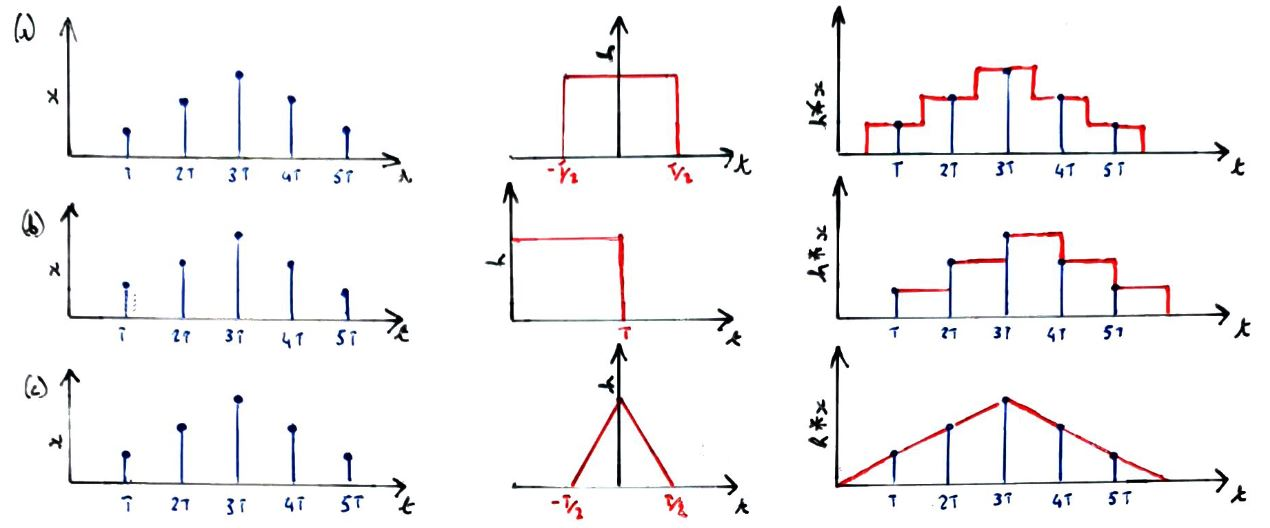
\includegraphics[width=\textwidth]{images/lecture_13_interpolation_filters.JPG}
  \caption{
  }
  \label{fig::lecture_13_interpolation_filters}
\end{figure}
%
A motivating example for why we need to be careful with our sampling of
an analog signal is given in Figure \ref{fig::lecture_13_aliasing}. Consider the sinusoid drawn in
black, whose frequency is higher than the sampling frequency (1.5 cycles
of the sinusoid elapse between discrete samples). Performing a smooth
interpolation of our discrete signal then recovers a sinusoid whose frequency
is lower than that which we originally sampled. We must place some
restrictions on our input signal so that we're not met with these types
of problem. A restriction that we'll find useful is that of a
\textbf{band-limited} signal, whereby there is some frequency $\omega_B$
such that
%
\begin{displaymath}
  X_c(\omega) = 0,\quad |\omega| > \omega_B \,.
\end{displaymath}
%
\begin{figure}[!htb]
  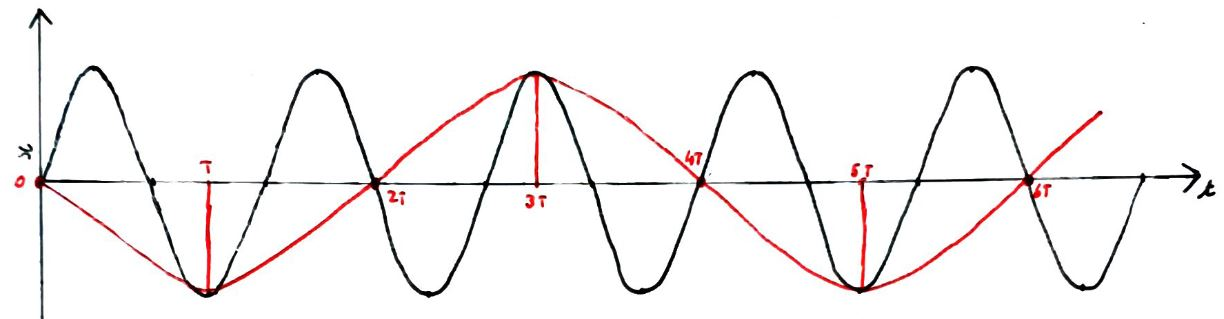
\includegraphics[width=\textwidth]{images/lecture_13_aliasing.JPG}
  \caption{
  }
  \label{fig::lecture_13_aliasing}
\end{figure}
%

\subsection{The Shannon-Nyquist Sampling Theorem}
%
A band-limited signal with maximum frequency $\omega_B$ can be perfectly
reconstructed from evenly-spaced samples if the sampling frequency
$\omega_s$ satisfies
%
\begin{equation}
  \omega_s > 2\omega_B \,,
\end{equation}
%
where $2\omega_B$ is referred to as the \textbf{Nyquist rate}.\\

Consider the act of sampling a continuous-time signal. This can be
written as the multiplication of the signal with an impulse train,
%
\begin{displaymath}
  x_s(t) = x(t) h(t) \,,
\end{displaymath}
%
where $x_s(t)$ is also a continuous-time signal which resembles
$x[n]$. We previously saw that for an impulse train, the Fourier
transform is given by $\frac{1}{T}$ for all spectral coefficients.
QQ Make sure this derivation is given in full.
Since we're working in radians, this becomes $\frac{2\pi}{T} = \omega_s$,
the separation between impulses being at $\frac{2\pi n}{T}$. As such,
%
\begin{displaymath}
  x_s(t) = x_c(t) h(t) \quad\Longleftrightarrow\quad
  X_s(\omega) = \frac{1}{2\pi}X_c(\omega) * H(\omega) \,.
\end{displaymath}
%
Note the factor of $\frac{1}{2\pi}$; this is to normalise the expression
for the Fourier transform of a periodic signal that we've previously
encountered,
%
\begin{displaymath}
  X(\omega) = \infsum{k}2\pi a_k\delta(\omega-k\omega_0) \,.
\end{displaymath}
%
Now, expanding out the frequency response,
%
\begin{displaymath}
  X_s(\omega) = \frac{1}{2\pi}X_c(\omega) * \left[
    \frac{2\pi}{T}\infsum{k}\delta(\omega - k\omega_s)
  \right] = \frac{1}{T}\infsum{k} X_c(\omega-k\omega_s) \,.
\end{displaymath}
%
Graphically (see Figure \ref{fig::lecture_13_nyquist}),
this means that $X_c(\omega)$ is scaled by
$\frac{1}{T}$ and duplicated each $k\omega_s$ units on the frequency axis.
Now, since the signal is band-limited, we see that the condition
$\omega_s - \omega_B > \omega_B \Longrightarrow \omega_s > 2\omega_B$
ensures that duplicates never overlap, and hence the inequality which
defines the sampling theorem.\\
%
\begin{figure}[!htb]
  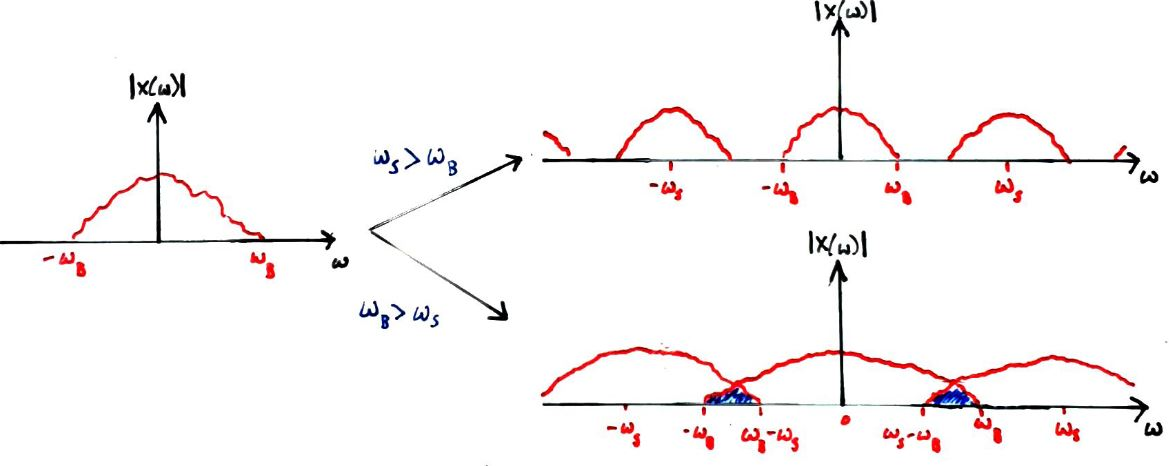
\includegraphics[width=\textwidth]{images/lecture_13_nyquist.JPG}
  \caption{
  }
  \label{fig::lecture_13_nyquist}
\end{figure}
%
To reconstruct our original analog signal $x_c(t)$, we need simply scale
$X_s(\omega)$ by $T$ and use a low-pass filter to remove all duplicates.
This means our reconstruction filter, $H_r(\omega)$, is a top hat function
on $\left[-\frac{\omega_s}{2},\frac{\omega_s}{2}\right]$ (or any shorter
duration) and height $T$. Inverse Fourier transforming then returns $x_c(t)$.
Any overlapping of duplicates in the frequency domain would result in higher
frequencies being combined with lower frequencies of copies, a phenomenon
referred to as \textbf{aliasing}. Note that while the CTFT is
$\omega_s$-periodic, the DTFT is $2\pi$-periodic, so replicas of $X(\omega)$
would be situated $2\pi$ apart on the frequency axis. The bandlimit, $\omega_B$
would be similarly scaled to appear at $\frac{2\pi\omega_b}{\omega_s} = \omega_B T$.\\

Thinking about this in the time domain, given $H_r(\omega)$ is a top hat on
$\left[-\frac{\omega_s}{2},\frac{\omega_s}{2}\right]$, the impulse response
$h_r(t)$ must be given by the sinc function
$h_r(t) = \sinc\left(\frac{\pi t}{T}\right)$, and the time-domain signal
we recover from the sampled signal is
%
\begin{displaymath}
  x(t) = x_s(t)*h_r(t) = \infsum{n} x[n]\sinc\left(\frac{\pi}{T}(t - nT)\right) \,.
\end{displaymath}
%
It's worth considering what this infinite sum of shifted sinc functions looks
like. It is graphed in Figure \ref{fig::lecture_13_sincs}.
At each discretely sampled point, a sinc
function is centred, but all other sincs in the summation are zero at integer
multiples of $T$. The values of $x(t)$ between integer multiples of $T$ are
given by the summation over an infinite number of sinc functions at that point.
%
\begin{figure}[!htb]
  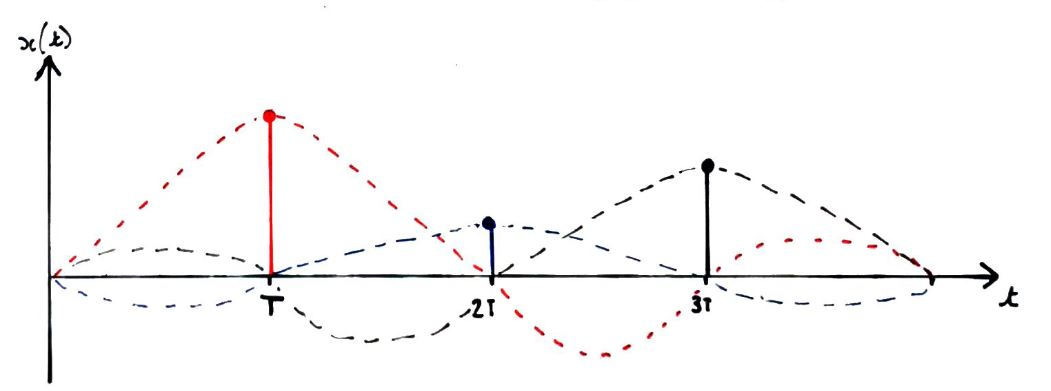
\includegraphics[width=\textwidth]{images/lecture_13_sincs.JPG}
  \caption{
  }
  \label{fig::lecture_13_sincs}
\end{figure}
%

\section{Lecture 14: Upsampling and Downsampling}

\subsection{Discrete-Time Processing of Continuous-Time Signals}
%
In the previous lecture, we have a continuous-time signal, $x_c(t)$ which, when
multiplied by the impulse train $d(t)$ yields a second continuous-time signal,
$x_s(t)$, whose non-zero values are spaced by $T$ in time and is, in effect,
a continuous-time version of a discrete-time signal. $x_s(t)$ would then be
converted into a discrete-time signal $x_d[n]$. We also showed that for the CTFT,
%
\begin{displaymath}
  X_s(\omega) = \frac{1}{T}\infsum{k}X_c(\omega - k\omega_s) \,,
\end{displaymath}
%
where $\omega_s = \frac{2\pi}{T}$. The DTFT of $x_d[n]$ is retrieved by simply
recalling that it is $2\pi$-periodic, and so the copies that appear in
$X_s(\omega)$ are spaced $2\pi$ apart rather than $\omega_s$. The next piece of
the puzzle involves the processing of $x_d[n]$ by some discrete-time system,
resulting in the output discrete-time signal $y_d[n]$. Finally, we may wish to
convert this back to a continuous-time signal, $y_r(t)$. Our question then is
how do we create the discrete-time system such that it behaves like the
frequency response of a continuous-time system.\\

We know that the frequency responses of the first analog-to-digital stage is
%
\begin{displaymath}
  X_d(\omega) = \frac{1}{T}\infsum{k}X_c\left(\frac{\omega - 2\pi k}{T}\right) \,,
\end{displaymath}
%
and that of the final digital-to-analog state is
%
\begin{displaymath}
  Y_r(\omega) = H_r(\omega)Y_d(\omega T) = \infsum{n} y_d[n]\sinc\left(\frac{t - nT}{T}\right) \,.
\end{displaymath}
%
The middle stage can be modelled as
%
\begin{displaymath}
  Y_d(\omega) = H(\omega)X_d(\omega) \,,
\end{displaymath}
%
where $H(\omega)$ is the general frequency-response of the discrete-time system.
We can simply bolt all of these stages together since the output of one
stage forms the input of another,
%
\begin{displaymath}
  Y_r(\omega) = H_r(\omega)Y_d(\omega T) = H_r(\omega)H(\omega)X_d(\omega)
  = H_r(\omega)H(\omega T)\frac{1}{T}\infsum{k}X_c\left(\omega -\frac{2\pi k}{T}\right) \,.
\end{displaymath}
%
Now, if we enforce the band-limit, such that for $|\omega| > \frac{\pi}{T}, X_c(\omega) = 0$,
then
%
\begin{displaymath}
  Y_r(\omega) = \left\{\begin{array}{ccl}
  H(\omega T)X_c(\omega) & & |\omega| < \frac{\pi}{T} \\
  0 & & \mathrm{otherwise}
  \end{array}\right. \,,
\end{displaymath}
%
since $H_r(\omega)$ is a band-pass filter. As such, the effective continuous-time frequency
response is
%
\begin{displaymath}
  Y_r(\omega) = H_{\mathrm{eff}}(\omega)X(\omega) \,,
\end{displaymath}
%
where
%
\begin{displaymath}
  H_{\mathrm{eff}}(\omega) = \left\{\begin{array}{ccl}
  H(\omega T) & & |\omega| < \frac{\pi}{T} \\
  0 & & \mathrm{otherwise}
  \end{array}\right. \,.
\end{displaymath}
%
Consequently, we can only design filters which are active when $|\omega| < \frac{\pi}{T}$,
else the reconstruction filter will remove any effects outside of this range; if we
want to make this interval wider, then we need to change the sampling rate.

\section{Lecture 15: Multirate Signal Processing and Polyphase Representations}
%
\subsection{Changing the Sample Rate By a Non-Integer Factor}
%
Previously, we discussed downsampling and upsampling by an integer rate.
For downsampling by a factor of $M$, we first prefiltered with a low-pass
filter with cutoff frequency $\pi/M$ and gain of $1$ to prevent aliasing,
then downsampled by $M$. For upsampling by a factor of $L$, we padded our
signal with $L-1$ zeroes between each of the original samples, then filtered
with a low-pass filter with cutoff frequency $\pi/L$ and gain of $L$
to interpolate.\\
%
Upsampling or downsampling by integer rates is rather restrictive; there are
many situations where we'd like to use non-integer rates. Consider changing
the sampling rate by the non-integer factor $\tau$, which can be written as
the quotient of two integers, $M/L$. We could in principle make some combination
of upsampling by $L$ and downsampling by $M$ to achieve this. So,
%
\begin{displaymath}
  x[n] \longrightarrow \boxed{\uparrow L}
  \longrightarrow \boxed{H_\mathrm{int}(\omega)}
  \longrightarrow \boxed{H_\mathrm{pre}(\omega)}
  \longrightarrow \boxed{\downarrow M}
  \longrightarrow x_\tau[n] \,.
\end{displaymath}
%
Note that the interpolating filter and prefilter can be condensed into a single
filter; in the frequency domain, we need simply multiply them together, which
results in a single low-pass filter whose cutoff frequency is dictated by
the smallest cutoff frequency of the other two,
%
\begin{displaymath}
  H_\tau(\omega) = H_\mathrm{int}(\omega)H_\mathrm{pre}(\omega)
  \quad \omega_c = \min\left(\frac{\pi}{M},\frac{\pi}{L}\right) \,.
\end{displaymath}
%
If $M>L$, we have a net reduction in sampling rate, meaning $H_\tau(\omega)$
is $H_\mathrm{pre}(\omega)$, and we need to prevent possible aliasing. If
$L>M$, we have a net increase in sampling rate, meaning $H_\tau(\omega)$ is
$H_\mathrm{int}(\omega)$, and we need to interpolate the signal. To give some
numbers, assume $\tau = 1.2$, then we need to upsample by a factor of $5$
and downsample by a factor of $6$, meaning we need to use
$H_\mathrm{pre}(\omega)$.

\subsection{The Noble Identities}
%
This strategy is problematic. Consider $\tau = 1.01$, where $M = 101$ and
$L = 100$, which seems rather wasteful since we're implementing large intermediate
changes in rate to retrieve a signal which is close to the original rate. We then
ask whether this process can be done more efficiently, to which the answer is of
course yes, and is referred to as \textbf{multirate signal processing}.
%
\begin{iden}[\textbf{The Noble Identity for Decimation}]
  The processes
  %
  \begin{displaymath}
    x[n] \longrightarrow \boxed{\downarrow M} \longrightarrow x_a[n]
    \longrightarrow \boxed{H(z)} \longrightarrow y_a[n]
  \end{displaymath}
  %
  and
  %
  \begin{displaymath}
    x[n] \longrightarrow \boxed{H\left(z^M\right)} \longrightarrow x_b[n]
    \longrightarrow \boxed{\downarrow M} \longrightarrow y_b[n]
  \end{displaymath}
  %
  are equivalent.\\

  Let's consider the meaning of $H(z^M)$ for a little insight:
  %
  \begin{displaymath}
    H(z^M) = \infsum{n} h[n]z^{-Mn} = \mathscr{Z}(h_e[n]) \,,
  \end{displaymath}
  %
  where $h_e[n]$ is a zero-padded version of $h[n]$, with $M-1$ zeroes between
  each sample. Recall that to transform between the $\omega$ and $z$ domains,
  we have the relationship
  %
  \begin{displaymath}
    X(\omega) = \left. X(z) \right|_{z = \ex{\im\omega}} \,.
  \end{displaymath}
  %
  Consequently, we can write the expression
  %
  \begin{displaymath}
    X_b(\omega) = H\left(z^M\right)X(\omega) = H\left(\ex{\im\omega M}\right)X(\omega)
    = H(\omega M) X(\omega)
  \end{displaymath}
  %
  since
  %
  \begin{displaymath}
    \left.H\left(z^M\right)\right|_{z=\ex{\im\omega}}
    = \infsum x[n]\ex{\im\omega nM} = H(\omega M) \,.
  \end{displaymath}
  %
  We saw in the previous lecture that the downsampling block of $X_b(\omega)$ results in
  %
  \begin{displaymath}
    Y_b(\omega) = \frac{1}{M}\sum_{m=0}^{M-1}X\left(\frac{\omega - 2\pi m}{M}\right)
    H(\omega - 2\pi m)
    = H(\omega)\frac{1}{M}\sum_{m=0}^{M-1} X\left(\frac{\omega - 2\pi m}{M}\right) \,,
  \end{displaymath}
  %
  since $H(\omega)$ is $2\pi$-periodic. But this is simply $H(\omega)$ multiplied by
  the result from having first downsampled by $X(\omega)$ by $M$, and consequently we
  have proven that $Y_b(\omega) = Y_a(\omega)$.
\end{iden}
%
\begin{iden}[\textbf{The Noble Identity for Interpolation}]
  The processes
  %
  \begin{displaymath}
    x[n] \longrightarrow \boxed{\uparrow L} \longrightarrow x_a[n]
    \longrightarrow \boxed{H(z)} \longrightarrow y_a[n]
  \end{displaymath}
  %
  and
  %
  \begin{displaymath}
    x[n] \longrightarrow \boxed{H\left(z^L\right)} \longrightarrow x_b[n]
    \longrightarrow \boxed{\uparrow L} \longrightarrow y_b[n]
  \end{displaymath}
  %
  are equivalent.\\

  Recall that upsampling shrinks the spectrum in the frequency domain by a factor
  $L$. Then
  %
  \begin{displaymath}
    Y_a(\omega) = X_a(\omega L) = X(\omega L)H(\omega L) \,,
  \end{displaymath}
  %
  and similarly
  %
  \begin{displaymath}
    X_b(\omega) = X(\omega L) \,,
  \end{displaymath}
  %
  meaning
  %
  \begin{displaymath}
    Y_b(\omega) = X(\omega L)H(\omega L) \,,
  \end{displaymath}
  %
  and we've proven that $Y_a(\omega) = Y_b(\omega)$. This seemingly innocent looking
  interchange has important computational consequences. If we upsample first, we increase
  our signal length by a factor of $L$, most of the elements being zero. This then
  results in a lot of redundant computation by the subsequent filter which has to
  process the signal in serial. In contrast, if we filter first, we have a significantly
  reduced computational overhead, which can later be upsampled.
\end{iden}

\subsection{The Polyphase Decomposition}
%
Consider some signal $h[n]$, an example of which is depicted in Figure QQ. We can think
of this sum as a sum of simpler signals; $h[n]$ is decomposed into a sum of $M$
subsequences $h_k[n]$, defined as follows,
%
\begin{displaymath}
  h_k[n] = h[k + nM] \,,
\end{displaymath}
%
which is the original sequence delayed by $k$ units and zero-padded with $M-1$ zeroes
between each of the originally sampled points. This is simplest to understand pictorially;
for $M=3$, pane (b) of Figure QQ shows the decomposition. We see that the original
signal is simply the summation of these subsequences,
%
\begin{displaymath}
  h[n] = \sum_{k=0}^{M-1}h_k[n-k] \,.
\end{displaymath}
%
Let $e_k[n]$ denote a corresponding $h_k[n]$ whose zero-padding has been removed, i.e.
$e_k[n] = h[nM + k] = h_k[nM]$. These are termed the polyphase components of $h[n]$.
Now, consider the Z-transform of $h[n]$ and split it into $M$ distinct sums,
%
\begin{align*}
  H(z) &= \infsum{k} h[k]z^{-k}
  = \infsum{\ell}h[\ell M]z^{-\ell M} + \infsum{\ell}h[\ell M+1]z^{-(\ell M + 1)} + \hdots \\
  &= \sum_{k=0}^{M-1}\infsum{\ell}h[\ell M + k]z^{-(\ell M + k)}
  = \sum_{k=0}^{M-1}z^{-k}\infsum{\ell}h[\ell M + k]z^{-\ell M} \\
  &= \sum_{k=0}^{M-1}z^{-k} \infsum{\ell}e_k[\ell]z^{-\ell M}
  = \sum_{k=0}^{M-1}z^{-k}\mathscr{E}_k\left(z^M\right) \,,
\end{align*}
%
where $\mathscr{E}_k\left(z^M\right)$ is the Z-transform of the $k\th$ polyphase
component shifted by $M$. Using this as a transfer function, we see that the
$k\th$ term in this summation is the input delayed by $k$ (since
$X(z)z^{-k} \Longleftrightarrow x[n-k]$) multiplied by the $k\th$ polyphase
component shifted by $M$, $\mathscr{E}\left(z^M\right)$. Each of these terms
is then summed to yield the output, $Y(z)$. This is the \textrm{polyphase realisation}
of $H(z)$.\\

\subsubsection{Polyphase Downsampling}
%
Now, let's think again about downsampling, where we prefiltered to prevent aliasing
then downsampled the signal. By using the polyphase realisation of our prefilter,
we can implement this as depicted in pane (a) of Figure QQ. The signal is passed
through $\mathscr{E}_0\left(z^M\right)$ on the first branch; on the second branch, it
is first delayed by the $z^{-1}$ block, then passed through $\mathscr{E}_1\left(z^M\right)$,
at which point it is summed with the result from the first branch. This is precisely
what the first two terms in the summation above represent, and proceeds up to
$\mathscr{E}_{M-1}\left(z^M\right)$. Once the summation has been completed, the
downsampling $M$ completes the process and we're left with our downsampled signal.\\
%
The polyphase realisation of the prefilter doesn't seem to have accomplished much;
consider a filter of length 400 that we downsample by a factor of 50; there are
then 50 polyphase components of the filter, each of length 8. For every value of the
input, this means we need to complete $8\times 50 = 400$ multiplications, exactly
the same had we kept the prefilter in its original form, albeit we've expressed
some parallelism. But we recall that the Noble identity for decimation allows
us to interchange the order of filtering and downsampling while changing the argument
of the filter from $z^M$ to $z$. This means we can implement the polyphase downsampling
as depicted in pane (b) of Figure QQ. Now since we downsample first, we pass $M$
times fewer values through each of the polyphase components, and our complexity
per input value becomes $400 / 8 = 50$ multiplications. So, the polyphase
downsampling lets us save a factor of $M$ in computational complexity. This is
a useful result since the larger the downsampling factor, the more data points
we're throwing away after having expended computational effort in prefiltering.
Now the complexity is independent of the downsampling factor, meaning we
don't waste effort.

\section{Lecture 16: FIR Filter Design Using Least-Squares}

\subsection{Ideal Filters}
%
So far, we've discussed generic systems with a transfer function or
frequency response, which transform some input signal into an output
signal. In the time domain, this involves convolution of the input
signal with an impulse response, while in the frequency domain, the
transfer function or frequency response is multiplied by the frequency
domain representation of the input signal, i.e.
%
\begin{displaymath}
  y[n] = x[n] * h[n] \quad\Longleftrightarrow\quad
  Y(\omega) = X(\omega)H(\omega) \,,
\end{displaymath}
%
where the magnitude and phase of the complex $Y(\omega)$ can be written
%
\begin{displaymath}
  |Y(\omega)| = |X(\omega)| \cdot |H(\omega)|
  \quad\mathrm{and}\quad
  \angle Y(\omega) = \angle X(\omega) + \angle H(\omega) \,,
\end{displaymath}
%
respectively. These are the two quantities that are plotted in a Bode
plot. A common frequency response that we've encountered is the
low-pass filter, given by
%
\begin{displaymath}
  H_\mathrm{lp}(\omega) = \rect{\frac{\omega}{\omega_c}} =
  \left\{\begin{array}{ccl}
  1 & & -\omega_c \leq \omega \leq \omega_c \\
  0 & & \mathrm{otherwise}
  \end{array}\right. \,,
\end{displaymath}
%
i.e. only the frequencies in the ``pass'' region are allowed through,
and are completely unmodified (not phase shifted).
We've also see that a pulse in the frequency-domain is a $\sinc$ in
the time domain, such that
%
\begin{displaymath}
  h_\mathrm{lp}[n] = \frac{\sin\left(\omega_c n\right)}{\pi n}
  = \sinc(\omega_c n) \,.
\end{displaymath}
%
Implementing this idealised low-pass filter presents us with some problems.
The first is that the $\sinc$ is not causal, and the second is that it
has infinite duration, neither of which we can realise in a physical system.\\

We have previously seen that for an ideal delay filter,
%
\begin{displaymath}
  h_\mathrm{d}[n] = \delta[n-n_d]
  \quad\Longleftrightarrow
  H_\mathrm{d}(\omega) = \ex{-\im\omega n_d} \,,
\end{displaymath}
%
where $n_d$ is some constant delay. The magnitude and phase of this
frequency response are simply
%
\begin{displaymath}
  |H_\mathrm{d}(\omega)| = 1 \quad\mathrm{and}\quad
  \angle H_\mathrm{d}(\omega) = -\omega n_d
\end{displaymath}
%
since $H(\omega) = |H(\omega)|\ex{\im\angle H(\omega)}$. We see that
the phase shift is a linear function of $\omega$; a filter with linear
phase then effectively delays the output by some number of units. This
isn't distortion since all frequencies are delayed by the same amount,
and the resultant interference pattern doesn't change, i.e. the output
sequence is just the input sequence shifted in time. In many cases, we
can't obtain a filter with zero phase (a filter which doesn't introduce
a delay into the signal). However, we are usually content with linear
phases.\\
%
Modifying our low-pass filter to have linear phase,
%
\begin{displaymath}
  H_\mathrm{lp}(\omega)
  = \ex{-\im\omega n_d}\rect{\frac{\omega}{\omega_c}} =
  \left\{\begin{array}{ccl}
  \ex{-\im\omega n_d} & & -\omega_c \leq \omega \leq \omega_c \\
  0 & & \mathrm{otherwise}
  \end{array}\right.
  \quad\Longleftrightarrow\quad
  h_\mathrm{lp}[n] = \frac{\sin(\omega_c(n-n_d))}{\pi(n-n_d)} \,.
\end{displaymath}
%
This suggests that, for the low-pass filter, we might be able to introduce
some delay $n_d$ which is large enough that the impulse response shifts
over to the right enough that $h[n-n_d]$ for $n<0$ is sufficiently
small as to not yield significant deviations in the output signal from the
desired output signal. However, while we've addressed the impulse response
not being causal, we've done nothing to address the infinite duration of
the impulse response.

\subsection{Group Delay}
%
We define the \textbf{group delay} as
%
\begin{displaymath}
  \tau_g = -\ddx{\omega} \arg H(\omega) \,.
\end{displaymath}
%
Consider the magnitude and phase of the frequency response of a
low-pass filter in panes (a) and (c) of Figure
\ref{fig::lecture_16_amplitude_response}. The discontinuities in the phase 
arise from the non-smooth points in the magnitude, i.e. where the frequency
response changes sign. Neither of these are desirable to work with from
an analytic point of view. Rather, the amplitude and ``properly unwrapped''
phase-shift, $A(\omega)$ and $\phi(\omega)$, respectively, are plotted in
panes (b) and (d) of Figure \ref{fig::lecture_16_amplitude_response},
which are both smooth and continuous,
%
\begin{displaymath}
  A(\omega) = \pm |H(\omega)| \quad\mathrm{and}\quad
  \phi(\omega) = \arg H(\omega) \,.
\end{displaymath}
%
We see then that since $\phi(\omega)$ is linear for an ideal filter, if the
group delay is approximately a constant, then the phase delay of the filter
is approximately linear.
%
\begin{figure}[H]
  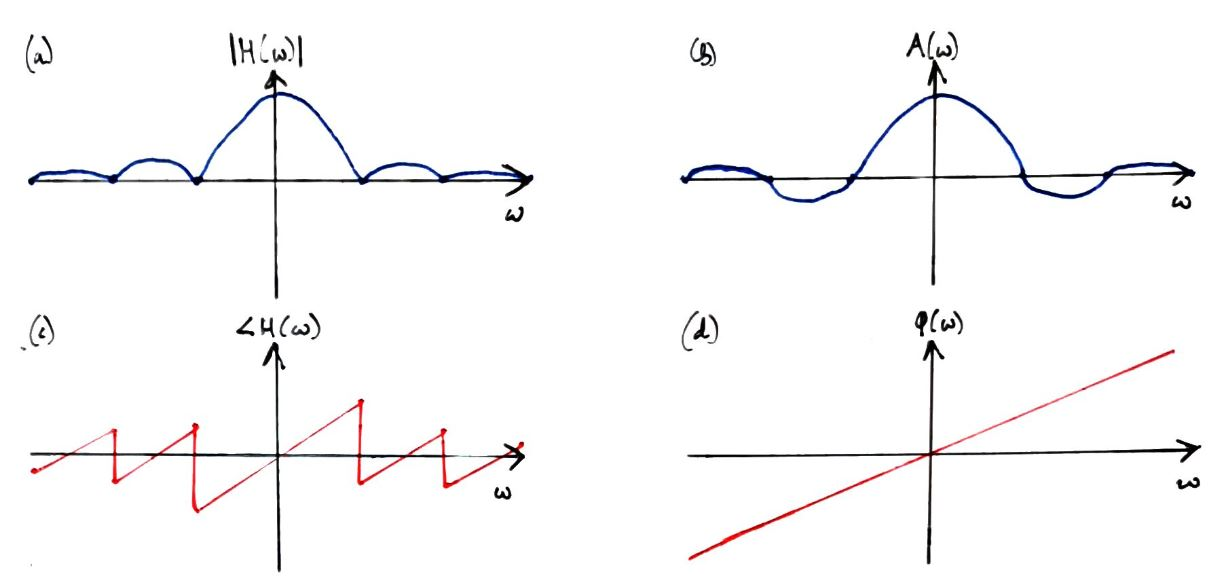
\includegraphics[width=\textwidth]{images/lecture_16_amplitude_response.JPG}
  \caption{In panes (a) and (c), the magnitude and phase responses of a filter,
    $|H(\omega)|$ and $\angle H(\omega)$ respectively, are shown. Note the
    discontinuities in $\angle H(\omega)$ which coincide with the points
    at which the magnitude response is not smooth. Panes (b) and (d) present
    the amplitude response and properly unwrapped phase-shift, $A(\omega)$ and
    $\phi(\omega)$ respectively, for the same filter; note that both are
    smooth and continuous, making their analytic treatment simpler.
  }
  \label{fig::lecture_16_amplitude_response}
\end{figure}

\subsection{Filter Design Process}
%
We have some desired frequency response, $H_\mathrm{des}(\omega)$, and we'd
like to approximate this as closely as possible using an approximate frequency
response which is constrained in form. Our filter design process can then
be enumerated as follows:
%
\begin{enumerate}
\item Choose a desired frequency response, $H_\mathrm{des}(\omega)$.
\item Choose an allowable class of filters (e.g. length-$N$ FIR filter).
\item Choose a measure of quality of the approximate filter.
\item Apply a method or algorithm which returns the optimal parameters of the
  filter.
\item Choose the best realisation of the filter (e.g. optimisation the implementation
  subject to some constraints, such as noise).
\end{enumerate}
%
In this lecture, we'll constrain our discussion to real, causal and digital filters
of the form
%
\begin{displaymath}
  H(z) = \frac{
    b_0 + b_1z^{-1} + b_2z^{-2} + \hdots + b_Mz^{-M}
  }{
    1 + a_1z^{-1} + a_2z^{-2} + \hdots + a_Nz^{-N}
  } \,,
\end{displaymath}
%
that have linear phase. If $\{a_i\} = 0$, then we have a FIR, or
\textbf{finite impulse response} filter, which by definition has no poles, otherwise we
have an IIR, or \textbf{infinite impulse response} filter. In general, we're
interested in the problem
%
\begin{displaymath}
  \min_{\{a\},\{b\}} \fnorm{E(z)} = \fnorm{H_\mathrm{des}(z) -
  \frac{
    b_0 + b_1z^{-1} + b_2z^{-2} + \hdots + b_Mz^{-M}
  }{
    1 + a_1z^{-1} + a_2z^{-2} + \hdots + a_Nz^{-N}
  }
  } \,.
\end{displaymath}
%
Consider $[n]$, a length-$N$ FIR filter, and assume it has linear phase
$\phi(\omega) = k_1 + k_2\omega$. Then,
%
\begin{align*}
  H(\omega) &= \sum_{n=0}^{N-1}h[n]\ex{-\im\omega n}
  = \ex{\im\omega M}\sum_{n=0}^{N-1}h[n]\ex{-\im\omega n}\ex{\im\omega M} \\
  &= \ex{\im\omega M}\sum_{n=0}^{N-1}h[n]\ex{\im\omega(M - n)} \,,
\end{align*}
%
where we've introduced the constant $M = \frac{N-1}{2}$. Now we note that there's
some kind of symmetry about the middle point in $h[n]$, e.g.
%
\begin{displaymath}
  h[0]\ex{\im\omega M} = h[0]\ex{\im\omega\frac{N-1}{2}} \,,
\end{displaymath}
%
and
%
\begin{displaymath}
  h[N-1]\ex{\im\omega M - \frac{N-1}{2}} = h[N-1]\ex{\im\omega\frac{N-1}{2} - \frac{N-1}{2}}
  = h[N-1]\ex{-\im\omega\frac{N-1}{2}} = h[N-1]\ex{-\im\omega M} \,.
\end{displaymath}
%
Now, we can generalise this,
%
\begin{align*}
  H(\omega) &= \ex{\im\omega M}\left(
  h[0]\ex{\im\omega M} + h[1]\ex{\im\omega(M-1)} + \hdots h[N-2]\ex{-\im\omega(M-1)} + h[N-1]\ex{-\im\omega M}
  \right) \\
  &= \ex{\im\omega M}(
  (h[0] + h[N-1])\cos(\omega M) + \im(h[0] - h[N-1])\sin(\omega M)\\
  &+ (h[1] + h[N-2])\cos(\omega (M - 1)) + \im(h[1] - h[N-2])\sin(\omega (M-1))\\
  &+ \hdots) \,.
\end{align*}
%
This slightly messy form is useful since we have a prefactor of $\ex{\im\omega M}$, i.e.
a linear phase, and a sum of sinusoids. We're now interested in when this can
be put in the form
%
\begin{displaymath}
  H(\omega) = A(\omega) \ex{\im(k_1 + k_2\omega)} \,,
\end{displaymath}
%
where $A(\omega)$ is real. Through comparison of terms, we see that the previous
expression for $H(\omega)$ is strictly real when the sine terms are zero, i.e.
when $h[n] = h[N-n-1]$, which implies that the filter must be symmmetric about
its middle element. Then
%
\begin{displaymath}
  A(\omega) = \sum_{m=0}^{M-1}2h[m]\cos(\omega(M-m)) + h[M]
\end{displaymath}
%
if $M$ is odd. So, if we have an odd-length filter which is symmetric about its
middle element, the filter will automatically have linear phase $\ex{-\im\omega M}$.
Similarly, if $M$ is even, there's a slightly different formula for the amplitude,
%
\begin{displaymath}
  A(\omega) = \sum_{m=0}^{\frac{N}{2}-1}2h[m]\cos(\omega(M-m)) \,,
\end{displaymath}
%
i.e. there's no DC term since the middle of the filter now occurs between
two filter values.\\

Now, since we know that choosing a symmetric impulse response we obtain a filter
with linear phase, we need only concern ourselves with their amplitude response.
There are four distinct types of filter with linear phase (i.e. their amplitude
responses are given by a summation of cosines), numbered Types I, II, III, and IV.
These are depicted in Figure \ref{fig::lecture_16_filter_types}.
Note that while Types II and IV appear to
contravene our requirement that the DTFT is $2\pi$-periodic, it's the magnitude
reponse that needs to be $2\pi$-periodic, rather than the amplitude response, which
is clearly satisfied here.\\
%
\begin{figure}[H]
  \includegraphics[width=\textwidth]{images/lecture_16_filter_Types.JPG}
  \caption{The four types of digital filter. In pane (a), a Type I filter
    is shown. Its amplitude response resembles a low-pass filter and is
    generated by a symmetric impulse response with an odd number of taps. In pane (b),
    a Type II filter is shown. Its amplitude response resembles a low-pass filter
    and is generated by a symmetric impulse response with an even number of taps.
    In pane (c), a Type III filter is shown. Its amplitude response resembles
    a band-pass filter and is generated by an antisymmetric impulse response
    with an odd number of taps. Finally, in pane (d) a Type IV filter is
    shown. Its amplitude response resembles a high-pass filter  and is generated
    by an antisymmetric impulse response with an even number of taps.
  }
  \label{fig::lecture_16_filter_types}
\end{figure}

\subsection{Quantifying the Quality of a Filter}
%
Consider some low-pass filter with cutoff frequency $\omega_c$. Typically,
we can't construct a filter with this idealised dropoff from the pass-band
to the stop-band at $\omega_c$. Rather, there's some transition region where
the pass-band transitions to the stop-band in some fashion. We'll refer to
the transition region by the domain $[\omega_1,\omega_2]$. One way we can
construct the filter is to specify its desired behaviour over the transition
region (see pane (b) of Figure \ref{fig::lecture_16_filter_quality}).
Alternatively, we can concern ourselves with the
quality of the pass-band and stop-band, and express no preference in the
form of the filter in the transition region (see pane (c) of
Figure \ref{fig::lecture_16_filter_quality}).\\
%
\begin{figure}[H]
  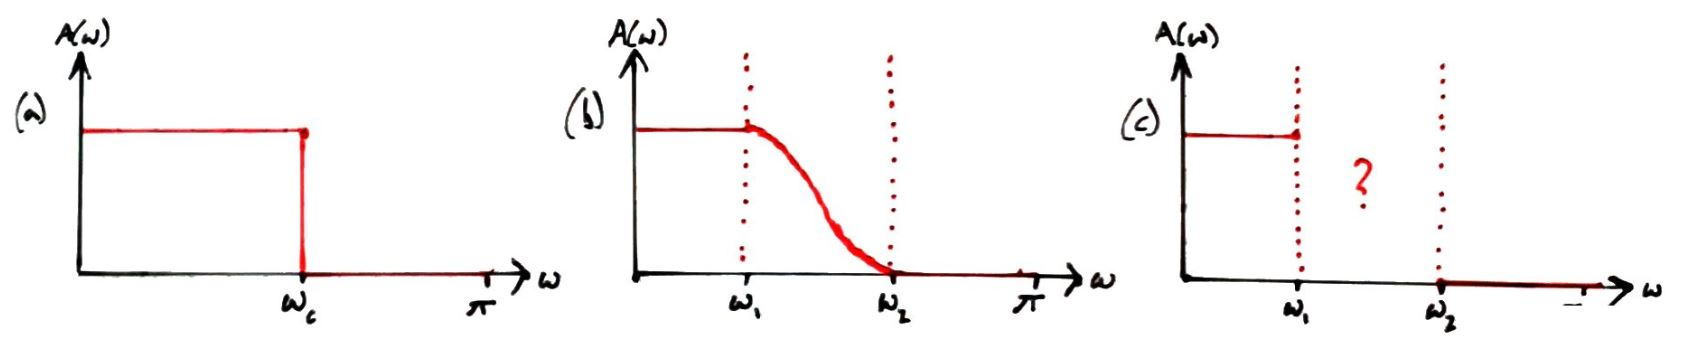
\includegraphics[width=\textwidth]{images/lecture_16_filter_quality.JPG}
  \caption{In pane (a), an idealised low-pass filter is shown with
    exact cutoff frequency of $\omega_c$. In pane (b), the behaviour of
    the transition region has been specified at the expense of poorer
    pass- and stop-band regions. In pane (c), the quality of the
    pass- and stop-band regions is prioritised, at the cost of
    having no control over the filter's form in the transition region.
  }
  \label{fig::lecture_16_filter_quality}
\end{figure}
%
We have a few metrics to quantify the quality of our constructed filter:
%
\begin{itemize}
\item (\textbf{Least-Square Approximation}) Average or squared error in the
  frequency domain. These are simple to implement but the filter may behave
  poorly in the transition region.
\item (\textbf{Chebyshev Approximation}) Maximum error over the pass-band or
  stop-band. These are more controllable in terms of the ripple of the filter,
  although it may take longer for the design process to converge.
\item (\textbf{Butterworth Filters}) A Taylor Series approximation to the
  desired response, sometimes referred to as ``maximally flat'', i.e. the function
  and all of its derivatives are as close to the desired filter as possible
  in a Taylor Series sense.
\end{itemize}

\subsection{Frequency Sampling Design of FIR Filters}
%
We now discuss the means by which we obtain the impulse response of the filter
from its amplitude response. We begin by taking $N$ equally spaced points on
the domain $[0,2\pi]$, i.e. the points $\omega_k = \frac{2\pi k}{N}$, where $N$
is the filter length. These samples are precisely those points that would be
taken with the DFT; the amplitude response can be acquired from the DTFT, which
the DFT samples. So, we can get an FIR filter that exactly interpolates these
samples with the IDFT,
%
\begin{displaymath}
  h[n] = \frac{1}{N}\sum_{k=0}^{N-1}H[k]\ex{\frac{\im 2\pi k n}{N}} \,.
\end{displaymath}
%
For a Type I filter, since we only care about the amplitude response,
%
\begin{displaymath}
  h[n] = \frac{1}{N}\left[
    A[0] + \sum_{k=1}^M 2A[k]\cos\left(\frac{2\pi(n-M)k}{N}\right)
  \right] \,.
\end{displaymath}
%
\begin{exmp}
  Consider a low-pass filter where $N=15$ (i.e. $M = \frac{N-1}{2} = 7$), and we
  have a desired cutoff frequency at $A_\mathrm{des}(\omega) = 0.4\pi$. The
  code given in \texttt{scripts/lecture\_16\_fir.py} constructs an approximation
  to the desired filter through use of frequency sampling. Its output is visualised
  in Figure \ref{fig::lecture_16_fir}.
  %
  \begin{figure}[H]
    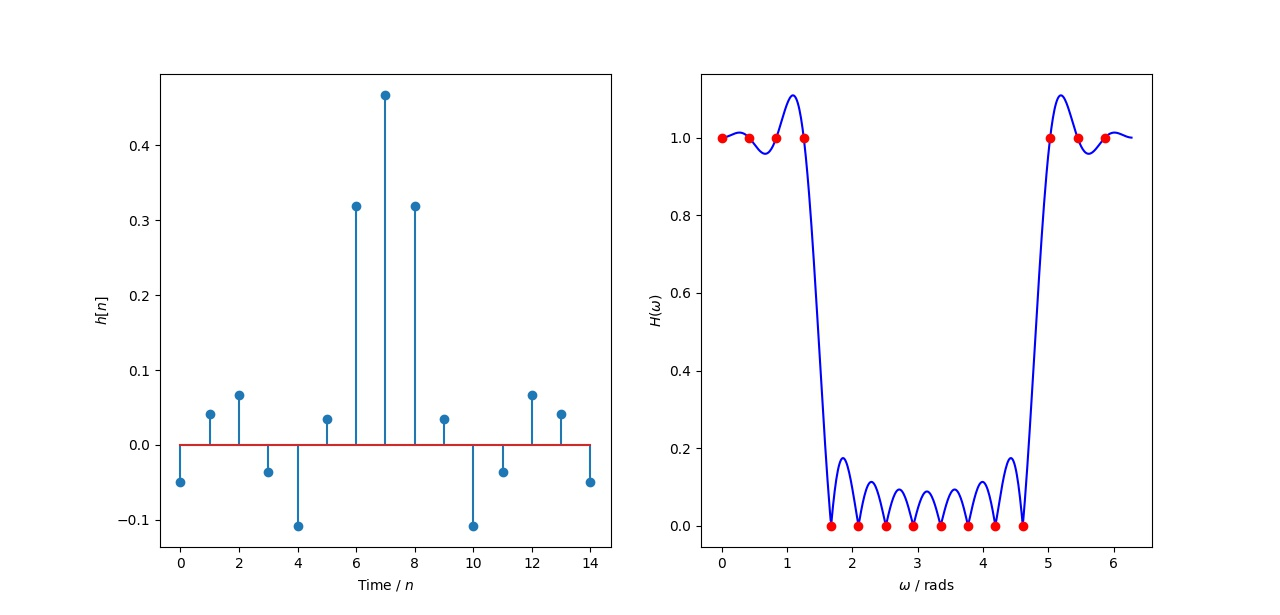
\includegraphics[width=\textwidth]{images/lecture_16_fir.JPG}
    \caption{The impulse response (left) and its frequency response
      (right) of a $15$-tap FIR filter constructed by frequency sampling.
      The sampled points are shown on the right as red circles; note that
      the interpolated frequency response passes exactly through these
      points.
    }
    \label{fig::lecture_16_fir}
  \end{figure}
  %
\end{exmp}
%
Consider the case where we wish to generate an $N$-tap FIR filter, but
using $L>N$ samples of the amplitude response. This yields an overdetermined
system of equations, and consequently has no unique solution. However,
we can use the method of ordinary least squares to find an approximate
solution,
%
\begin{displaymath}
  E = \sum_{k=0}^{L-1}\fnorm{A(\omega_k) - A_\mathrm{des}(\omega_k)}^2 \,,
\end{displaymath}
%
where $\omega_k = 2\pi k/L$. By recalling Parseval's Theorem, it transpires
that this error can be interpreted in the time-domain,
%
\begin{displaymath}
  E = \sum_{k=0}^{L-1} \fnorm{h[n] - h_\mathrm{des}[n]}^2 \,,
\end{displaymath}
%
where $h_\mathrm{des}[n]$ is the length-$L$ FIR filter which goes through
the $L$ samples (as per the previous example). To minimise, we then choose
$h[n]$ to agree with $h_\mathrm{des}[n]$ on the middle $N$ filter taps, i.e.
like truncating $h_\mathrm{des}[n]$. So we find the best length-$L$ filter,
and ``chop out'' the middle $N$ taps, which provides us with the best
length-$N$ approximation to $h_\mathrm{des}[n]$. This filter will have
a different frequency response to one constructed from $N$ samples of
the desired amplitude response, but ultimately will be better since
it provides an improved solution to the least-squares minimisation.

\subsection{Non-Uniform Frequency Sampling Design of FIR Filters}
%
It's possible to use $N$ non-uniformly spaced samples of the
amplitude response to construct the corresponding impulse response, but we
would not be able to use the IDFT for this. It's best to think about
this in terms of matrix algebra, where
%
\begin{displaymath}
  A(\omega) = \sum_{m=0}^{M-1}2h[n]\cos(\omega(M-m)) + h[M]
\end{displaymath}
%
is written
%
\begin{displaymath}
  \left[\begin{array}{c} A(\omega_0) \\ A(\omega_1) \\ \vdots \\ A(\omega_{L-1})\end{array}\right]
  =
  \left[\begin{array}{cccc}
      2\cos(\omega_0 M) & 2\cos(\omega_0 (M-1)) & \hdots & 1 \\
      2\cos(\omega_1 M) & 2\cos(\omega_1 (M-1)) & \hdots & 1 \\
      \vdots & \vdots & \ddots & \vdots \\
      2\cos(\omega_{L-1} M) & 2\cos(\omega_{L-1} (M-1)) & \hdots & 1      
    \end{array}\right]
  \left[\begin{array}{c} h[0] \\ h[1] \\ \vdots \\ h[M]\end{array}\right]
\end{displaymath}
%
\begin{displaymath}
  \mathbf{a} = \mathbf{Fh} \,,
\end{displaymath}
%
where $\mathbf{a}\in\mathbb{R}^L$, $\mathbf{h}\in\mathbb{R}^{M+1}$ and
$\mathbf{F}\in\mathbb{R}^{L\times(M+1)}$. If $\mathbf{F}$ is square, i.e.
$M+1 = L$, then $\mathbf{h} = \mathbf{F}^{-1}\mathbf{a}$, otherwise the
least-squares solution requires that the pseudoinverse be used,
%
\begin{displaymath}
  \mathbf{h} = \left(\mathbf{F}^\top\mathbf{F}\right)^{-1}\mathbf{F}^\top\mathbf{a} \,.
\end{displaymath}
%
Being able to use non-uniform samples of the amplitude response is useful
for directing our sampling of the amplitude response to those regions that
we're particularly concerned about replicating. For instance, if we'd like
the pass-band, which terminates at $\omega_1$, and the stop-band, which
begins at $\omega_2$, to be as close to the desired amplitude response as
possible, we can direct all of our sampling to these regions, at the cost
of placing no constraints on the transition region,
$\omega_1\leq \omega \leq\omega_2$. Similarly, if there are certain
points of the desired amplitude response that we really want to replicate
as closely as possible, we can introduce some weights into the least-squares
minimisation
%
\begin{displaymath}
  E = \sum_{k=0}^{L-1}w_k\fnorm{A(\omega_k) - A_\mathrm{des}(\omega_k)}^2 \,,
\end{displaymath}
%
and in terms of the matrix formulation,
%
\begin{displaymath}
  \mathbf{h} = \left(\mathbf{F}^\top\mathbf{F}\right)^{-1}
  \mathbf{F}^\top\mathbf{W}\mathbf{a} \,.
\end{displaymath}
%
where $\mathbf{W}$ is the diagonal weight matrix.

\section{Lecture 17: FIR Filter Design (Chebyshev)}

In the previous lecture, we spoke about FIR filter design using the
least-squares approximation; we specified a number of points in
a desired filter's amplitude response and created a filter which
interpolated between these points. This scheme can be problematic
since it doesn't allow us to specify the form of the filter
between the interpolated points; the ripple is something that we
can't really control. The focus of this lecture is to provide a
scheme whereby the created filter doesn't deviate by more than
some specified amount in the pass-band and stop-band.\\
%
To this end, we introduce a different error function from the
least-squares version. Define the Chebyshev cost function as
%
\begin{displaymath}
  \min E = \max_{\omega\in[0,\pi)} \lvert A(\omega) - A_\mathrm{des}(\omega)\rvert \,,
\end{displaymath}
%
i.e. over the range $[0,\pi)$, the filter error is defined as the
maximum deviation between the desired filter and the filter we've
created. Filters that are optimal with respect to this criterion
are called \textbf{Equiripple}. An equiripple filter is presented
in Figure \ref{fig::lecture_17_equiripple}. We can define some
tolerance in the ripple in the
passband and stopband, and as long as the filter length is
compatible with these specifications, we can drive the filter
response to being as desired.\\
%
\begin{figure}[!htb]
  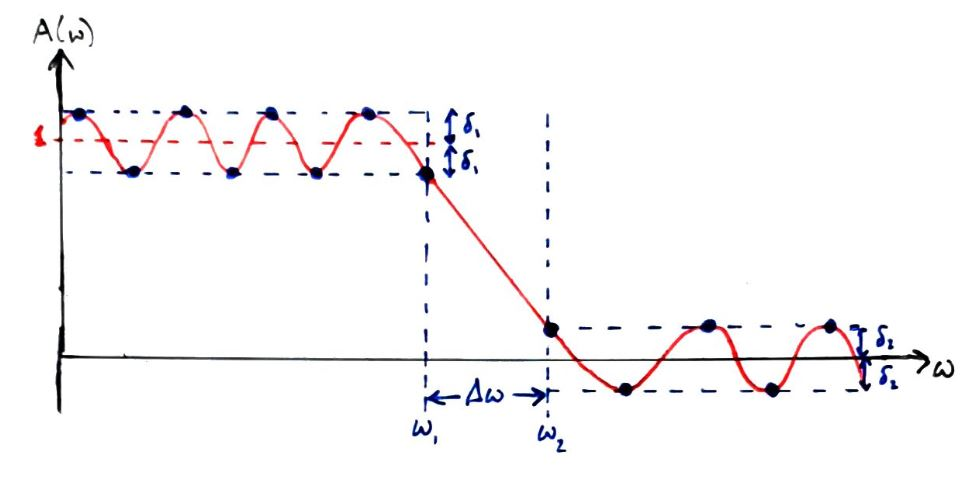
\includegraphics[width=\textwidth]{images/lecture_17_equiripple.JPG}
  \caption{A parameterised equiripple filter. The tolerances in the
    pass-band and stop-band are denoted by $\delta_1$ and $\delta_2$
    respectively, while the transition region, $\omega_1\leq\omega\leq\omega_2$
    is of width $\Delta\omega$. Note that this filter has 13
    extremal frequencies, meaning its impulse response has 25 taps.
  }
  \label{fig::lecture_17_equiripple}
\end{figure}
%
An acceptable frequency response has the following characteristics:
%
\begin{enumerate}
\item Linear phase FIR filters (since the filter is real, anti/symmetric
  and only introduce delays into the output).
\item Some width, $\Delta\omega$, of the transition band.
\item Deviation from $1$ in the pass-band of $\pm\delta_1$.
\item Deviation from $0$ in the stop-band of $\pm\delta_2$.
\end{enumerate}

Before progressing, it is worth introducing the Chebyshev polynomials
of the first kind,
%
\begin{displaymath}
  T_n(x) = \cos\left(n\cos^{-1}x\right) \quad\Longleftrightarrow\quad
  T_n(\cos \theta) = \cos n\theta \,.
\end{displaymath}
%
From the double-angle formulae, we know that
%
\begin{displaymath}
  \cos 0\theta = 1, \quad \cos 1\theta = \cos\theta, \quad \cos 2\theta = 2\cos^2\theta + 1, \hdots \,,
\end{displaymath}
%
allowing us to conclude that
%
\begin{displaymath}
  T_0(x) = 1, \quad T_1(x) = x, \quad T_2(x) = 2x^2 + 1, \hdots \,,
\end{displaymath}
%
i.e. $\cos(n\theta)$ is some $n\th$ order polynomial in $x = \cos\theta$.
As such, for some generic sum of cosines,
%
\begin{displaymath}
  S(x) = \sum_{n=0}^{N-1} c_n\cos(n\theta)
  = \sum_{n=0}^{N-1}c_n\cos(n\cos^{-1}x)
  = \sum_{n=0}^{N-1} d_nT_n(x) \,.
\end{displaymath}
%
This equivalence between cosines and polynomials (and sums thereof) presents
a change of variables that we'll find useful later in this lecture.

\subsection{The Approximation Problem}
%
Previously, we showed that the amplitude response of a Type I linear
phase filter can be written as some linear combination of cosines 
%
\begin{displaymath}
  A(\omega) = \sum_{k=0}^{r-1}c_k \cos(\omega k) \,,
\end{displaymath}
%
where $r=\frac{N+1}{2}$. Our aim now is to minimise the Chebyshev cost
function subject to the constraint that our amplitude response be
given by the above linear combination of cosines. The
\textbf{approximation problem} can then be written as, given
%
\begin{enumerate}
\item A set of frequency bands in $[0,\pi]$.
\item A desired real-valued $A_\mathrm{des}(\omega)$ in these bands.
\item A positive weight function, $W(\omega)$.
\item The form $A(\omega) = \sum_{k=0}^{r-1}c_k \cos(\omega k)$
\end{enumerate}
%
find $\{c_k\}$. To do this, we need to solve using the
\textbf{alternation theorem}: if $A(\omega)$ is a sum of $r$ cosines,
then a necessary and sufficient condition for $A(\omega)$ to be the
unique best-weighted Chebyshev (equiripple) approximation to
$A_\mathrm{des}(\omega)$ on the given bands is that
%
\begin{displaymath}
  E(\omega) = W(\omega)\lvert A(\omega) - A_\mathrm{des}(\omega) \rvert
\end{displaymath}
%
must exhibit at least $r+1$ extremal frequencies in the given bands,
where extremal frequencies are some $\{\omega_i\}$ such that
%
\begin{displaymath}
  E(\omega_i) = \max E(\omega) \quad\mathrm{and}\quad E(\omega_i) = -E(\omega_{i+1}) \,.
\end{displaymath}
%
This is depicted in Figure \ref{fig::lecture_17_equiripple}
for a length-25 FIR filter (i.e. $r+1 = \frac{N+1}{2} = 13$. If we
recognise that there are $r+1$ extremal frequencies in a filter, then
we can say that the filter is optimal with respect to the Chebyshev
cost function.

\subsection{The Remez Exchange Algorithm}
%
The Remez exchange algorithm is an iterative process for finding
an optimal equiripple filter by first guessing its extremal
frequencies, and iterating until our constraints are met. Consider
our cost function,
%
\begin{displaymath}
  E(\omega) = A_\mathrm{des}(\omega) - \sum_{k=0}^{r-1}c_k\cos(\omega k) \,,
\end{displaymath}
%
which can be made to take on the values $\pm\delta$ for any given set
of frequency bands $\{\omega_1,\hdots,\omega_{r+1}\}$, i.e.
%
\begin{equation}\label{eq::remez}
  A_\mathrm{des}(\omega_m) = \sum_{k=0}^{r-1}\cos(\omega_m k) + (-1)^m\delta \,,
\end{equation}
%
for all $i = 1, \hdots, r+1$. There exists a unique solution to this
for the combination of $\{c_k\}$ and $\delta$.\\
%
Consider an initial set of guesses for the extremal frequencies,
$T_0 = \{\omega_1,\hdots,\omega_{r+1}\}$. The Remez Exchange Algorithm
then follows:
%
\begin{enumerate}
\item Solve the linear equations in Equation \ref{eq::remez}, the solution of
  which has an error that oscillates with amplitude $\delta_k$ on the
  extremal frequencies $T_k$.
\item Interpolate to find the frequency response on all of $[0,\pi]$.
\item Search $[0,\pi]$ to see if and where the magnitude of the error
  exceeds $\delta_k$.
\item If the maximum error is equal to $\delta_k$, we are done. Otherwise,
  take the $r+1$ maximal frequencies in this new frequency response as
  $T_{k+1}$ and return to the first step.
\end{enumerate}
%
\begin{exmp}
  Try to approximate $A_\mathrm{des}(\omega) = x^2$ by $A(\omega) = d_0 + d_1 x$
  over $[0,1]$ using the Chebyshev cost function. In other words, solve
  %
  \begin{displaymath}
    \min_{d_1,d_2}E = \max_{\omega\in[0,1]}\lvert x^2 - (d_0 + d_1 x)\rvert \,.
  \end{displaymath}
  %
  Since we have a second order polynomial in $x$, we are looking for 3 extremal
  frequencies. To begin the Remez exchange algorithm, begin by guessing
  $T_0 = \{1/4, 1/2, 1\}$, the points at which we make the error oscillate, i.e.
  %
  \begin{displaymath}
    x_k^2 = d_0 + d_1x_k + (-1)^k\delta \,,
  \end{displaymath}
  %
  where $d_0, d_1, \delta$ are unknown. This can be formulated as three equations
  in three unknowns,
  %
  \begin{displaymath}
    \left[\begin{array}{ccc}
        1 & x_0 & (-1)^0 \\
        1 & x_1 & (-1)^1 \\
        1 & x_2 & (-1)^2
      \end{array}\right]
    \left[\begin{array}{c}d_0 \\ d_1 \\ \delta \end{array}\right]
    = \left[\begin{array}{c}x_0^2 \\ x_1^2 \\ x_2^2\end{array}\right]
  \quad\longrightarrow\quad
    \left[\begin{array}{ccc}
        1 & \frac{1}{4} & 1 \\
        1 & \frac{1}{2} & -1 \\
        1 & 1 & 1
      \end{array}\right]
    \left[\begin{array}{c}d_0 \\ d_1 \\ \delta \end{array}\right]
    = \left[\begin{array}{c}\frac{1}{16} \\ \frac{1}{4} \\ 1\end{array}\right]  
  \end{displaymath} \,,
  %
  which when solved yields $d_0 = -5/16, d_1 = 5/4, \delta = 1/16$. The
  cost function for this is plotted in Figure
  \ref{fig::lecture_17_remez_iteration}. We see that at the
  points $T_0$, we indeed have an error of $\delta = 1/16$, but this is
  by no means the smallest error on the domain $[0,\pi]$; rather,
  $\max_{[0,\pi]}E(x) = E(0) = 5/16$, and consequently we need to iterate
  the Remez exchange, this time using $T_1 = \{0, 5/8, 1\}$, those values of
  $x$ where $E(x)$ is extremal,
  %
  \begin{displaymath}
    \left[\begin{array}{ccc}
        1 & 0 & 1 \\
        1 & \frac{5}{8} & -1 \\
        1 & 1 & 1
      \end{array}\right]
    \left[\begin{array}{c}d_0 \\ d_1 \\ \delta \end{array}\right]
    = \left[\begin{array}{c}0 \\ \frac{25}{64} \\ 1\end{array}\right] \,,  
  \end{displaymath}
  %
  which when solved yields $d_0 = -15/128, d_1 =1, \delta =15/128$. The
  cost function for this is plotted in Figure \ref{fig::lecture_17_remez_iteration}.
  As before, we see
  that $\max_{[0,\pi]}E(x) = E(1/2) = 17/128$, which is greater than
  $\delta$, and consequently we set $T_2 = \{0, 1/2, 1\}$,
  %
  \begin{displaymath}
    \left[\begin{array}{ccc}
        1 & 0 & 1 \\
        1 & \frac{1}{2} & -1 \\
        1 & 1 & 1
      \end{array}\right]
    \left[\begin{array}{c}d_0 \\ d_1 \\ \delta \end{array}\right]
    = \left[\begin{array}{c}0 \\ \frac{1}{4} \\ 1\end{array}\right] \,,  
  \end{displaymath}
  %
  which when solved yields $d_0 = -1/8, d_1 = 1, \delta = 1/8$, the cost function of
  which is plotted in Figure \ref{fig::lecture_17_remez_iteration}. Now we see that
  the extremal frequencies
  are indeed $T_2$, and the Remez exchange algorithm has converged. The best
  approximation is then $A(x) = d_0 + d_1 x = - \frac{1}{8} + x$.
  %
  \begin{figure}[!htb]
    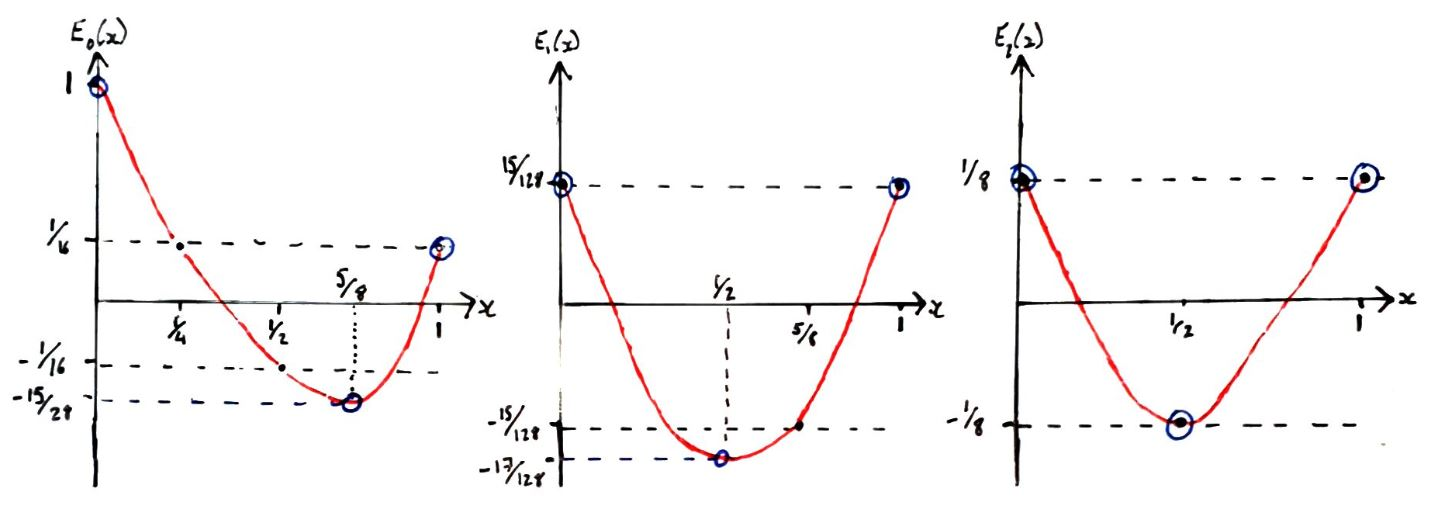
\includegraphics[width=\textwidth]{images/lecture_17_remez_iteration.JPG}
    \caption{An example of manually performing the Remez exchange algorithm
      to find an $A(\omega) = d_0 + d_1 x$ that best approximates
      $A_\mathrm{des}(\omega) = x^2$.
    }
    \label{fig::lecture_17_remez_iteration}
  \end{figure}

\end{exmp}
%
The Remez Exchange Algorithm always converges to an equiripple approximation,
\textbf{but} it may not have the desired pass-band and stop-band characteristics for
a given filter order. For instance, we can't make the ripple arbitrarily small
given only 3 filter taps; we can only do so well with a finite number of
parameters.\\
%
To characterise an equiripple filter, one needs to know the filter length, $N$,
its pass-band and stop-band edges, $\omega_1$ and $\omega_2$, and the pass-band
and stop-band deviations, $\delta_1$ and $\delta_2$. Given that the filter of
length $N$ might not be able to converge to this specification, we can invoke a
heuristic, to calculate the $N$ which satisfies these criteria,
%
\begin{displaymath}
  N \approx \frac{-20 \log_10\sqrt{\delta_1\delta_2} - 13}{14.6(\omega_2 - \omega_1)} + 1 \,.
\end{displaymath}
%
As the pass-band and stop-band are brought closer together, $\omega_2 - \omega_1$
becomes smaller and $N$ increases as we might expect. Similarly if we want
the deviation to increase, $\delta_1\delta_2$ increases and the
filter also increases. Signal processing toolboxes obviously offer
a means to design filters using the Remez Exchange Algorithm,
the Parks-McClellan algorithm is one such variant of an iterative
means to find the optimal Chebyshev FIR filter given a parameterisation.
%
\begin{exmp}
  Consider a low-pass filter where $N=11$ where $\omega_1 = 0.3\pi$ and
  $\omega_2 = 0.5\pi$. The code given in \texttt{scripts/lecture\_17\_remez.py}
  invokes the Remez exchange algorithm to approximate the desired FIR filter.
  Its output is visualised in Figure \ref{fig::lecture_17_remez_example}.
  %
  \begin{figure}[!htb]
    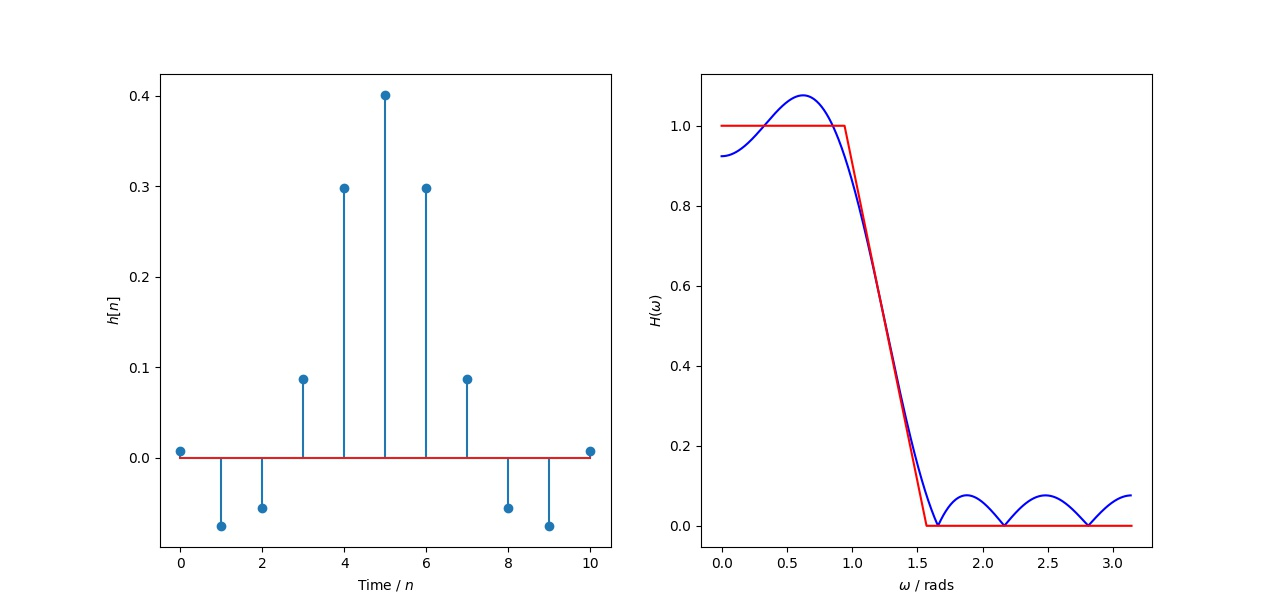
\includegraphics[width=\textwidth]{images/lecture_17_remez_example.JPG}
    \caption{The impulse response (left) and its frequency response
      (right) of an $11$-tap FIR filter constructed by the Remez exchange
      algorithm. The desired amplitude response is shown by the red
      curve in the figure on the right.
    }
    \label{fig::lecture_17_remez_example}
  \end{figure}
  %
\end{exmp}

\subsection{FIR Advantages and Disadvantages}
%
The advantages of using an FIR filter include:
%
\begin{enumerate}
\item We can achieve exactly linear phase filters; there's always
  some midpoint in the filter about which it is symmetry. This is
  not the case with an IIR filter since there is no midpoint, which
  consequently leads to some kind of distortion.
\item Easy and efficient implementation.
\item Easily designed with linear methods.
\item Filters are always stable since there are no poles, by definition.
\end{enumerate}
%
The disadvantages of using an FIR filter include:
%
\begin{enumerate}
\item May require a large number of taps, $N$, in the filter to achieve good
  approximations to some frequency responses (see the heuristic in
  the previous section). This is problematic for real-time processing since
  it's undesirable to introduce a large delay, $N$ between input and
  output.
\item May need many operations per output, and may need to store
  a lot of coefficients, which is constraining for some embedded systems.
\end{enumerate}

\section{Lecture 18: IIR Filter Design}
%
Recall that the infinite impulse response (IIR) is written
as some combination of input and previous output values,
%
\begin{displaymath}
  y[n] = \sum_{m=0}^M b[m]x[n-m] - \sum_{k=1}^N a[k]y[n-k] \,,
\end{displaymath}
%
where the first summation is simply a FIR filter, and the convolutional
sum between $a$ and $y$ begins at $k=1$ since we assume $a[0] = 1$,
the multiplier of $y[n]$ on the LHS. The transfer
function, as we have previously seen, is given by
%
\begin{displaymath}
  H(z) = \infsum{n}h[n]z^{-n}
  = \frac{\sum_{m=0}^M b[m]z^{-m}}{\sum_{n=0}^N a[n]a^{-n}}
  = \frac{B(z)}{A(z)} \,.
\end{displaymath}
%
There are several differences with FIR filters:
%
\begin{enumerate}
\item IIR filters do not have linear phase; a linear phase
  was obtained as a result of the symmetry of the impulse response,
  but since this is of infinite duration for an IIR filter, there
  is no central point about which the impulse response can be
  symmetric since we require that the filter be causal.
\item IIR filters have low orders relative to their FIR counterparts,
  and are sufficient to implement ``tight'' filter specifications, e.g.
  very steep dropoff in the transition region.
\item We typically start by designing an analog filter, then convert
  this to digital.
\end{enumerate}
%
The design process for an IIR filter is broadly the same as that for
and FIR filter; we begin by selecting some desired frequency
response, $H_\mathrm{des}(\omega)$, then choose the class of filter we'd like
to use (e.g. IIR filter of order $N$ in both numerator and
denominator). A distance measure, or error, is then chosen between
$H(\omega)$ and $H_\mathrm{des}(\omega)$. The optimal filter in the
class which minimises this distance measure.

\subsection{Direct Digital IIR Design: Prony's Method}
%
Given a desired IIR, $h_\mathrm{des}[n]$, where $0\leq n < \infty$, we
find the coefficients $a[k]$ and $b[m]$, such that $h_\mathrm{des}[n]$
is best approximated by 
%
\begin{displaymath}
  y[n] = - \sum_{k=1}^N a[k]y[n-k] + \sum_{m=0}^M b[m]x[n-m] \,.
\end{displaymath}
%
Now, we have
%
\begin{displaymath}
  H_\mathrm{des}(z) = \infsum{n}h_\mathrm{des}[n]z^{-n}
  \quad\mathrm{and}\quad
  H(z) = \frac{B(z)}{A(z)}
  = \frac{b_0 + b_1z^{-1} + \hdots + b_Mz^{-M}}{1 + a_1z^{-1} + \hdots + a_Nz^{-N}} \,,
\end{displaymath}
%
meaning that if $H(z) = H_\mathrm{des}(z)$, it must follow that
$H(z)A(z) = B(z)$. Then, by polynomial multiplication
%
\begin{displaymath}
  \left(h[0] + h[1]z^{-1} + h[2]z^{-2} + \hdots\right)
  \left(1 + a_1z^{-1} + \hdots + a_Nz^{-N}\right)
  =
  \left(b_0 + b_1z^{-1} + \hdots + b_Mz^{-M}\right)
\end{displaymath}
%
and matching up powers of $z$, we have that:
%
\begin{displaymath}
  h[0] = b_0, \quad
  h[1] + h[0]a_1 = b_1, \quad
  h[2] + h[1]a_1 + h[0]a_2 = b_2, \quad \hdots \,,
\end{displaymath}
%
or in matrix form,
%
\begin{displaymath}
  \left[\begin{array}{c} b_0 \\ b_1 \\ \vdots \\ b_M \\ 0 \\ \vdots \\ 0 \end{array}\right]
  =
  \left[\begin{array}{cccccc}
      h_0 & 0 & 0 & \hdots & 0 & 0 \\
      h_1 & h_0 & 0 & \hdots & 0 & 0 \\
      \vdots & \vdots & \vdots & \ddots & \vdots & \vdots \\
      h_N & h_{N-1} & h_{N-2} & \vdots & h_1 & h_0 \\
      \vdots & \vdots & \vdots & \ddots & \vdots & \vdots \\
      h_K & h_{K-1} & h_{K-2} & \vdots & h_{K-N+1} & h_{K-N}
    \end{array}\right]
  \left[\begin{array}{c} 1 \\ a_1 \\ a_2 \\ \vdots \\ a_{N-1} \\a_N \end{array}\right] \,,
\end{displaymath}
%
such that $\mathbf{b}\in\mathbb{R}^{K+1}$, $\mathbf{a}\in\mathbb{R}^{N+1}$
and $\mathbf{H}\in\mathbb{R}^{(K+1)\times(N+1)}$, where $\mathbf{H}$
contains the elements of $h_\mathrm{des}[n]$. Writing this in a partitioned
matrix form,
%
\begin{displaymath}
  \left[\begin{array}{c}\mathbf{b}_* \\ \mathbf{0} \end{array}\right] =
  \left[\begin{array}{c|c}
      \multicolumn{2}{c}{\mathbf{H}_1} \\
      \hline
      \mathbf{h} & \mathbf{H}_2
    \end{array}\right]
  \left[\begin{array}{c}1 \\ \mathbf{a}_* \end{array}\right] \,,
\end{displaymath}
%
where $\mathbf{b}_*\in\mathbb{R}^{M+1}$ is the non-zero part of $\mathbf{b}$,
$\mathbf{a}_*\in\mathbb{R}^N$ are the non-unity coefficients of $\mathbf{a}$,
$\mathbf{H}_1\in\mathbb{R}^{(N+1)\times(M+1)}$,
$\mathbf{H}_2\in\mathbb{R}^{(K-M)\times N}$ and $\mathbf{h}\in\mathbb{R}^{K-M}$.
Now, we can write out a set of linear equations,
%
\begin{align*}
  \mathbf{b}_* &= \mathbf{H}_1\mathbf{a}_* \\
  \mathbf{0} &= \mathbf{h} + \mathbf{H}_2\mathbf{a}_* \,.
\end{align*}
%
If $K - M = N$, then $\mathbf{H}_2$ is square and we can solve for
$\mathbf{a}_*$ through inversion; this simply means that the IIR
impulse response has $M+N+1$ values. Once $\mathbf{a}^*$ has been
computed, then we can directly compute $\mathbf{b}_*$ from the
first equation, i.e.
%
\begin{displaymath}
  \mathbf{a}_* = -\mathbf{H}_2^{-1}\mathbf{h}
  \quad\mathrm{and}\quad
  \mathbf{b}_* = -\mathbf{H}_1\mathbf{H}_2^{-1}\mathbf{h} \,.
\end{displaymath}
%
This is Prony's Method, and was actually developed in the $18\th$
century for chemistry, but was impractical until the advent of
digital computers. If the desired impulse response $h_\mathrm{des}[n]$
has more values than $M+N+1$, then $\mathbf{H}_2$ is not square, and
we have to use the pseudoinverse, which solves the system in a least-squares
sense, i.e. it solves
%
\begin{displaymath}
  \left[\begin{array}{c}\mathbf{b}_* \\ \mathbf{0} \end{array}\right]
  + \mathbf{e} =
  \left[\begin{array}{c|c}
      \multicolumn{2}{c}{\mathbf{H}_1} \\
      \hline
      \mathbf{h} & \mathbf{H}_2
    \end{array}\right]
  \left[\begin{array}{c}1 \\ \mathbf{a}_* \end{array}\right] \,,
\end{displaymath}
%
where $\mathbf{e}$ is some error vector whose norm $\fnorm{\mathbf{e}}_2$
is minimised; when $\mathbf{H}_2$ is square and invertible, this
error vector is zero, otherwise
%
\begin{displaymath}
  \mathbf{a}_* = -\left(\mathbf{H}_2^\top\mathbf{H}_2\right)^{-1}\mathbf{H_2}^\top\mathbf{h}
  \quad\mathrm{and}\quad
  \mathbf{b}_* = -\mathbf{H}_1\left(\mathbf{H}_2^\top\mathbf{H}_2\right)^{-1}\mathbf{H_2}^\top\mathbf{h} \,.
\end{displaymath}
%
Rather than minimisation with respect to $\fnorm{\mathbf{e}}_2$, we'd like
to minimise with respect to an error that's more representative of
the quality of our IIR filter, $\hat{e}[n] = h[n] - h_\mathrm{des}[n]$.
This is a difficult non-linear optimisation problem requiring some
heuristic, and is not discussed here.

\subsection{Digital IIR Design: Frequency-Sampling}
%
Consider the case where we have a desired frequency response,
$H_\mathrm{des}(\omega)$. Again, we're looking to find the best
$a, b$ which satisfy
%
\begin{displaymath}
  H(z) = \frac{B(z)}{A(z)} \,,
\end{displaymath}
%
where $B(z)$ has $M+1$ unknowns and $A(z)$ has $N$ unknowns. Let
$L = M + N$; given $L + 1$ unknowns, we need $L + 1$ samples
of the frequency response to solve. As with the FIR frequency
sampling, sample the frequency response at the points
$\omega_k = \frac{2\pi k}{L + 1}$. These are simply the samples
we'd obtain from taking the DFT of $h_\mathrm{des}[n]$, and so
%
\begin{displaymath}
  H[k] = \frac{B[k]}{A[k]} \quad\Longleftrightarrow B[k] = H[k]A[k] \,,
\end{displaymath}
%
where $H[k], B[k], A[k]$ are the length-$L+1$ DFTs of $h[n], b[n], a[n]$,
respectively. Hence,
%
\begin{displaymath}
  b = h \circledast a \,,
\end{displaymath}
%
and writing out this circular convolution explicitly,
%
\begin{displaymath}
  \left[\begin{array}{c} b_0 \\ b_1 \\ \vdots \\ b_M \\ 0 \\ \vdots \\ 0 \end{array}\right]
  =
  \left[\begin{array}{ccccc}
      g_0 & g_L & g_{L-1} & \hdots & g_1 \\
      g_1 & g_0 & \ddots  & \hdots & g_2 \\
      g_2 & g_1 & \ddots  & \hdots & g_3 \\ 
      \vdots & \vdots & \ddots & \hdots & \hdots \\
      g_L & g_{L-1} & \hdots  & g_1 & g_0 \\ 
    \end{array}\right]
  \left[\begin{array}{c} 1 \\ a_1 \\ \vdots \\ a_N \\ 0 \\ \vdots \\ 0 \end{array}\right] \,,
\end{displaymath}
%
where each $g_k$ is the IDFT of $H_\mathrm{des}\left(\frac{2\pi k}{L + 1}\right)$.
This looks very similar to the matrix equation we encountered in the Prony Method,
except this time the elements in the transformation matrix are samples of
the desired frequency response rather than impulse response. Consequently,
we can perform the same matrix partitioning as before,
%
\begin{displaymath}
  \left[\begin{array}{c}\mathbf{b}_* \\ \mathbf{0} \end{array}\right] =
  \left[\begin{array}{c|c}
      \multicolumn{2}{c}{\mathbf{G}_1} \\
      \hline
      \mathbf{g} & \mathbf{G}_2
    \end{array}\right]
  \left[\begin{array}{c}1 \\ \mathbf{a}_* \end{array}\right] \,,
\end{displaymath}
%
where $\mathbf{b}_*\in\mathbb{R}^{M+1}$ is the non-zero part of $\mathbf{b}$,
$\mathbf{a}_*\in\mathbb{R}^N$ are the non-unity coefficients of $\mathbf{a}$,
$\mathbf{G}_1\in\mathbb{R}^{(N+1)\times(M+1)}$,
$\mathbf{G}_2\in\mathbb{R}^{(K-M)\times N}$ and $\mathbf{g}\in\mathbb{R}^{K-M}$.
Now, we can write out a set of linear equations,
%
\begin{align*}
  \mathbf{b}_* &= \mathbf{G}_1\mathbf{a}_* \\
  \mathbf{0} &= \mathbf{g} + \mathbf{G}_2\mathbf{a}_* \,,
\end{align*}
%
and extend to use the pseudoinverse if we take more than $L+1$ samples of
the desired frequency response.\\
%
As with the FIR case, since we're interpolating between samples of
$H_\mathrm{des}(\omega)$, we have no control on the behaviour of the
filter between the sampled points.
Note that $H_\mathrm{des}(\omega)$ should be consistent with a real $h_d[n]$, so
that $a[n]$ and $b[n]$ are also real. However, there are no guarantees that
the designed filter is stable (since the IIR has poles), which is a guarantee
with the FIR case.

\subsection{Digital IIR Design from Analog IIR Filter}
%
This is the most common means of digital IIR design; there existed a large
corpus of work on optimal, closed-form analog filters before the advent of digital
electronics, and consequently it's prudent to use one of these analog
filters as the basis for an optimal digital filter. As with the
FIR filters, there are four major types of analog IIR filter which are
graphed in Figure \ref{fig::lecture_18_analog_filters}.\\
%
\begin{figure}[!htb]
  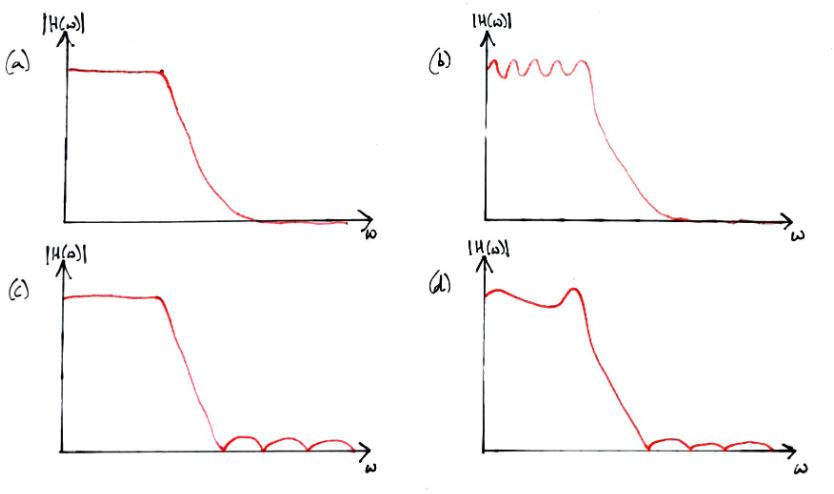
\includegraphics[width=\textwidth]{images/lecture_18_analog_filters.JPG}
  \caption{Four main types of analog filter. In pane (a), a Butterworth
    filter is shown which has frequency response as flat as possible in the
    pass-band (also referred to as a maximally flat magnitude filter). In
    pane (b), a Type I Chebyshev filter is shown, which has ripple in the
    pass-band but is flat in the stop-band. In pane (c), a Type II Chebyshev
    filter is shown, which has ripple in the stop-band but is flat in the
    pass-band. Finally, in pane (d) an elliptic filter is shown, which
    has equialised ripple in both the pass-band and stop-band (also
    referred to as a Cauer filter). The elliptic filter has a sharper cutoff
    than the others, at the expense of ripples on the whole bandwidth.
  }
  \label{fig::lecture_18_analog_filters}
\end{figure}
%
The problem is how to convert these continuous-time closed-form solution to
the digital time case. We suggest taking the continuous-time cases;
the impulse response $h_c(t)$ and its Laplace transform $H_c(s)$, and
sampling them at some rate to produce the discrete-time impulse response
$h[n]$ and its Z-transform $H(z)$. However, this is not trivial. For
$H_c(s)$ to be stable, its poles need to be contained to the left of the
imaginary axis, whereas for $H(z)$ to be stable, the poles need to be
contained within the unit circle. Performing this transformation requires
a complex conformal mapping, which is beyond the scope of these notes.\\
%
There are two main approaches to converting the continuous-time filters
to discrete time.

\subsubsection{Impulse Invariance}
%
Given some continuous-time impulse response $h_c(t)$, create a discrete-time
counterpart by sampling at rate $1/T$ and scale by $T$, such that
$h[n] = Th_c(nT)$. As we saw in the lecture on multirate processing, taking
this to the frequency domain with the DTFT yields a magnitude response which
is $2\pi$-periodic, and the cutoff frequency is scaled to $\omega_c T$.
Similarly, if we do not sample at a high enough rate, the periodic copies of
$|H(\omega)|$ might alias which is problematic since it fundamentally changes
the filter and will likely no longer be optimal in the digital world.

\subsubsection{The Bilinear Transformation}
%
This is much safer than impulse invariance. Consider the transformation
between the $s$ and $z$ domains,
%
\begin{displaymath}
  s = \frac{2}{T}\frac{z-1}{z+2} \quad\mathrm{and}\quad
  z = \frac{\frac{2}{T} + s}{\frac{2}{T} - s}
\end{displaymath}
%
Some examples of this \textbf{bilinear transformation} are presented in
Figure \ref{fig::lecture_18_bilinear_transform}.
%
\begin{figure}[!htb]
  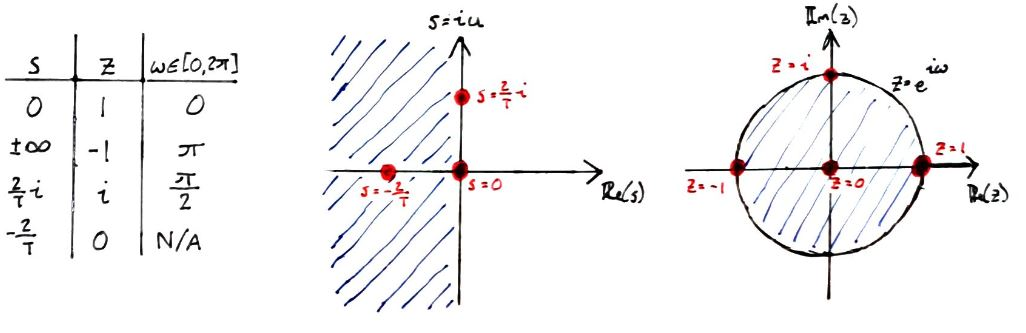
\includegraphics[width=\textwidth]{images/lecture_18_bilinear_transform.JPG}
  \caption{Examples of the bilinear transform between the $s$ and
    $z$ domains. Note that for the imaginary axis in the $s$ domain,
    $\im u$, $u$ is the continuous-time frequency with infinite range.
    The positive part of the $\im u$ axis wraps around to
    $0 \leq \omega \leq \pi$ in the $z$ domain, while the negative
    part of the $\im u$ axis wraps around to $-\pi \geq \omega \geq 0$
    in the $z$ domain. The hatched regions are those areas of the respective
    domains where the transforms don't converge; the left-half plane in
    the $s$ domain maps to the interior of the unit circle in the $z$ domain.
  }
  \label{fig::lecture_18_bilinear_transform}
\end{figure}
%
Consider the magnitude responses of the analog and digital filters in
Figure \ref{fig::lecture_18_prewarp}. These two filters are equivalent;
the cutoff frequency in the analog case transforms to some other
cutoff frequency in the digital case. Consequently, one has to take
steps to make sure the cutoff of the analog filter is chosen so as
to produce the desired cutoff in the digital filter.\\
%
The main idea is then to prewarp the desired digital filter cutoff
frequencies to the corresponding analog cutoffs using the $z\rightarrow s$
transformation. We then design an analog filter using this prewarped
cutoff frequency and warp back to a digital filter using the $s\rightarrow z$
transformation. If we comply with our filter specification in the
analog world (e.g. stop-band ripple, pass-band ripple, etc.), then
the digital filter will also comply to these specifications since
the bilinear transform only maps the domain; the responses will
stay the same -- a ripple in the $s$ domain will simply be squeezed
on stretched in the $z$ domain, its magnitude will not change.
%
\begin{figure}[!htb]
  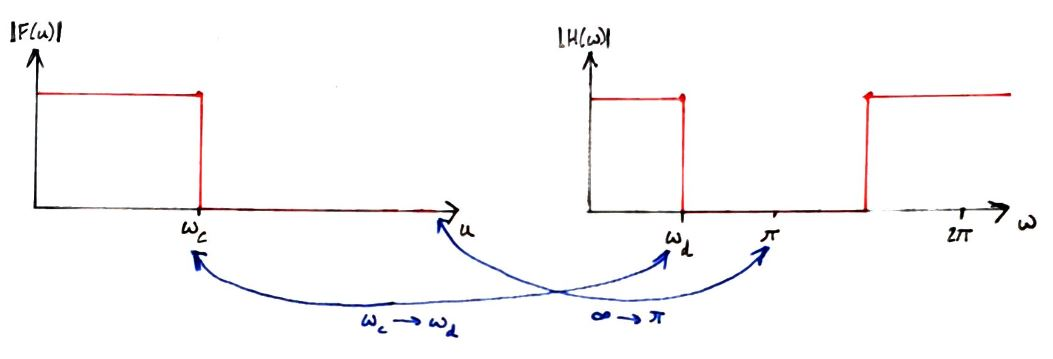
\includegraphics[width=\textwidth]{images/lecture_18_prewarp.JPG}
  \caption{The magnitude responses of an analog filter (left) and its
    digital counterpart (right). Under the
    bilinear transformation, $\omega_c\rightarrow\omega_d$. Also note
    that the mapping from $u=\infty$ to $z=\pi$ is shown.
  }
  \label{fig::lecture_18_prewarp}
\end{figure}
%


%%%
%%% Appendices
%%%
\newpage
\begin{appendices}
\section{Decibels}
%
When dealing with the power content of a signal, we are typically presented with enormous
dynamic ranges spanning many orders of magnitude; picowatts and below all the way to
gigawatts and above. Relative powers spanning this range are cumbersome to work with.
For instance, if I have a signal whose energy is 6 millwatts and amplify it to 5 megawatts,
the amplification is given by their ratio, the gain,
%
\begin{displaymath}
  \mathrm{Gain}\; = \frac{P_{out}}{P_{in}} = \frac{5\times 10^6}{6\times 10^{-3}}
  \approx 8.3\times 10^8 \,.
\end{displaymath}
%
The simplest way to overcome this is to invoke a logarithmic scale for relative
powers, resulting in a value on the Bel scale,
%
\begin{displaymath}
  \mathrm{Gain}\;\mathrm{(Bel)}\; = \log_{10}\left(\frac{P_{out}}{P_{in}}\right)
  = \log_{10}\left(\frac{5\times 10^6}{6\times 10^{-3}}\right) \approx 8.9\; \mathrm{Bel} \,.
\end{displaymath}
%
A quirk of history means that we typically work with decibels rather than Bels,
%
\begin{displaymath}
  \mathrm{Gain}\;\mathrm{(dB)} = 10\log_{10}\left(\frac{P_{out}}{P_{in}}\right)\; \mathrm{dB} \,,
\end{displaymath}
%
the reason being that the smallest detectable difference in volume by a human is
a decibel, which has led to its use in other fields by convention. There is another
scale which uses the natural logarithm, the Neper Scale, but this has never gained
traction. Inverting our expression for the gain to recover the power of the output signal,
%
\begin{displaymath}
  \log_{10}\left(\frac{P_{out}}{P_{in}}\right) = \frac{\mathrm{Gain}}{10}
  \quad\rightarrow\quad
  P_{out} = 10^{\frac{Gain}{10}}P_{in} \,.
\end{displaymath}
%
In signal processing, another common unit is the ``decibel milliwatt'', or dBm, where
the reference input power is equal to a milliwatt,
%
\begin{displaymath}
  \mathrm{Gain}\;\mathrm{(dBm)} = 10\log_{10}\left(\frac{P_{out}}{1\mathrm{mW}}\right)\; \mathrm{dBm} \,.
\end{displaymath}
%
A second useful feature of these logarithmic ratios is the fact that multiplication
of gains in the dimensionless scale we first introduced becomes addition.
%
\begin{exmp}
  Consider an initial signal with power $7$dBm, which is amplified by an amplifier with
  a gain of 2. In dBm,
  %
  \begin{displaymath}
    10\log_{10}\left(\frac{2\mathrm{mW}}{1\mathrm{mW}}\right) \approx 3\mathrm{dBm} \,.
  \end{displaymath}
  %
  The power of the resultant signal is simply given by the sum of the initial signal power
  and the gain of the amplifier, $7\mathrm{dBm}\; + 3\mathrm{dBm}\; = 10\mathrm{dBm}$.
\end{exmp}
%
It is worth considering the form of the gain in units of decibels -- it is plotted
in Figure \ref{fig::appendix_1_decibels}. Note that when the input and output signals
have the same power, the gain is equal to $1$dB. In keeping with the additive property
of decibels, any decrease in gain is given by a negative number.
%
\begin{figure}[!htb]
  \begin{tikzpicture}
    \begin{axis}[
        width=0.9\textwidth,
        axis lines=middle,
        xmin=0, xmax=10, ymin=-10, ymax=10,
        xlabel=$\frac{P_{out}}{P_{in}}$,
        ylabel=$\mathrm{Gain}\;\mathrm{(dB)}$
      ]
      \addplot[samples=100, domain=0:15, blue, ultra thick] {10*log10(x)};
    \end{axis}
  \end{tikzpicture}
  \caption{The ratio of output to input signals plotted against the associated
    gain in dB. Observe that a ratio of 2, i.e. the output signal has a power twice
    that of the input signal, the gain is 3dB.}
  \label{fig::appendix_1_decibels}
\end{figure}


\section{The Singular Value Decomposition}

Consider the matrix $\matr{X}\in\mathbb{R}^{n\times m}$, which is the
concatenation of a series of $m$ vectors, $\vec{x}_1,\hdots,\vec{x}_m$,
%
\begin{displaymath}
  \matr{X} = \left[\begin{array}{cccc}
      \vdots & \vdots & & \vdots \\
      \vec{x}_1 & \vec{x}_2 & \hdots & \vec{x}_m \\
      \vdots & \vdots & & \vdots
    \end{array}\right] \,,
\end{displaymath}
%
where $\vec{x}\in\mathbb{R}^n$. We assume that $n\gg m$. Each of these vectors
describes a sample from some sample space, e.g. a picture of a face, the
matrix $\matr{X}$ then collecting all such pictures together into a dataset.
Another more pertinent example might be each $\vec{x}$ denoting the state of
a system at a particular time (e.g. the frequency content), and the
collection $\matr{X}$ represents the time evolution of the system.\\

The \textbf{Singular Value Decomposition} (SVD) allows us to decompose the
matrix $\matr{X}$ into the product of three matrices,
%
\begin{equation}
  \matr{X} = \matr{U}\matr{\Sigma}\matr{V}^\top \,,
\end{equation}
%
where $\matr{U}\in\mathbb{R}^{n\times n}, \matr{V}\in\mathbb{R}^{m\times m}$
are unitary, and $\matr{\Sigma}\in\mathbb{R}^{n\times m}$ is diagonal.
The SVD for a matrix $\matr{X}$ is guaranteed to exist and is unique.
We also have that the diagonal elements of $\matr{\Sigma}$ are ordered in
magnitude and non-negative, such that
$\sigma_1 \geq \sigma_2 \geq \hdots \geq \sigma_m \geq 0$. To introduce some
explicit notation, $\matr{U}$ are the left singular vectors of $\matr{X}$,
$\matr{V}$ are the right singular vectors of $\matr{X}$ and $\matr{\Sigma}$
are the singular values corresponding to the singular vectors.\\

Each of these matrices has an associated physical intuition. The left singular
vectors are the basis vectors in which the samples in $\matr{X}$ can be fully
expressed (both a sample in $\matr{X}$ and a left singular vector are in
$\mathbb{R}^n$, and $n$ basis vectors are required to fully describe the
associated vector space, hence $\matr{U}\in\mathbb{R}^{n\times n}$. The singular
values $\sigma_k$ express the ``importance'' of the combination of $\vec{u}_k$
and $\vec{v}_k$ in describing $\matr{X}$. Finally, the right singular vectors
quantify the content of each of the left singular vectors across the samples in
$\matr{X}$. However, we use the transpose of $\matr{V}$, and so the rows are
the quantities to which we should be ascribing intuition. The columns of
$\matr{V}^\top$ quantify the amount of each basis state to make an $\vec{x}$,
i.e. the first column of $\matr{V}^\top$ describes how to make $\vec{x}_1$, and
so on.\\

The product of matrices in the SVD can be written as a sum of outer
products,
%
\begin{displaymath}
  \matr{U}\matr{\Sigma}\matr{V}^\top
  = \sum_{i=1}^m \vec{u}_i\sigma_i\vec{v}_i^\top
\end{displaymath}
%
Since $\matr{X}$ only comprises $m$ vectors in an $n$-dimensional vector field,
it's impossible to infer all of these basis states which space $\mathbb{R}^{n\times n}$,
as the left singular vectors appear to claim to do. It transpires that only
the first $m$ left singular vectors are meaningful -- the remaining $n-m$
are to be discarded by virtue of the associated singular values being equal to zero.
Consequently, when performing the SVD, we need only take the $\mathbb{R}^{n\times m}$
sub-matrix of $\matr{U}$ and the $\mathbb{R}^{m\times m}$ sub-matrix of $\matr{\Sigma}$,
which we'll denote with a caret,
%
\begin{displaymath}
  \matr{X} = \hat{\matr{U}}\hat{\matr{\Sigma}}\matr{V}^\top \,,
\end{displaymath}
%
which is referred to as the ``economy'' SVD and is typically the desired
option since $n\gg m$, meaning the discarded sub-matrices are rather large.
Note that each term in the summation over outer products yields a rank-one
matrix, as per the definition of the rank of an outer product of vectors
(it is formed from a linearly independent row and column, but every row
and column in the outer product is formed from these, leading to all
rows and columns in the outer product being linearly dependent).\\

So, our SVD is a linear combination of rank-one matrices, each one scaled
by a singular value, which effectively quantifies the importance of the
term to the construction of $\matr{X}$. Typically, the SVD is truncated
at some term $r$, beyond which point the singular values diminish the
contribution of the corresponding outer products to being negligible.
This truncated SVD is only approximately equal to $\matr{X}$,
%
\begin{displaymath}
  \matr{X} \approx \tilde{\matr{X}}
  = \tilde{\matr{U}}\tilde{\matr{\Sigma}}\tilde{\matr{V}}^\top \,,
\end{displaymath}
%
where $\tilde{\matr{U}}\in\mathbb{R}^{r\times n}$,
$\tilde{\matr{\Sigma}}\in\mathbb{R}^{r\times r}$ and
$\tilde{\matr{V}}\in\mathbb{R}^{r\times m}$. This is formalised in the
Eckart-Young theorem [1936], which states that
%
\begin{equation}
  \argmin_{\mathrm{rank}(\tilde{\matr{X}}) = r}
  \fnorm{\matr{X} - \tilde{\matr{X}}}
  = \tilde{\matr{U}}\tilde{\matr{\Sigma}}\tilde{\matr{V}}^\top \,,
\end{equation}
%
i.e. the best rank-$r$ approximation to $\matr{X}$ is given by the
SVD truncated to the $r\th$ term. Hence a key function of the SVD --
compression and matrix approximation. Since
$\tilde{\matr{U}}, \tilde{\matr{\Sigma}}, \tilde{\matr{V}}$ contain
far fewer elements than $\matr{X}$, they provide an excellent means to
compress $\matr{X}$, albeit with some losses dictated by the truncation
order $r$. Note that the truncated matrices
$\tilde{\matr{U}}$ and $\tilde{\matr{V}}$ are no longer unitary. Rather,
%
\begin{displaymath}
  \tilde{\matr{U}}^\top\tilde{\matr{U}} = \matr{I}_{r\times r},\quad
  \tilde{\matr{U}}\tilde{\matr{U}}^\top \neq \matr{I}_{n\times n} \,,
\end{displaymath}
%
and
%
\begin{displaymath}
  \tilde{\matr{V}}\tilde{\matr{V}}^\top = \matr{I}_{r\times r},\quad
  \tilde{\matr{V}}^\top\tilde{\matr{V}} \neq \matr{I}_{n\times n} \,,
\end{displaymath}
%
as one would expect -- matrices of rank $r < n$ cannot be orthonormal
in $\mathbb{R}^{n\times n}$.\\

The matrix $\matr{X}^\top\matr{X}\in\mathbb{R}^{m\times m}$ is a columnwise
correlation matrix, describing the correlation between columns, or samples,
in the matrix $\matr{X}$, the diagonal being the autocorrelation of samples.
As with all correlation matrices, it is positive semi-definite with real
eigenvalues. Computing this correlation matrix using the economy SVD,
%
\begin{displaymath}
  \matr{X}^\top\matr{X} =
  \matr{V}\hat{\matr{\Sigma}}^\top\hat{\matr{U}}^\top
  \hat{\matr{U}}\hat{\matr{\Sigma}}\matr{V}^\top
  = \matr{V}\hat{\matr{\Sigma}}^2\matr{V}^\top \,,
\end{displaymath}
%
by virtue of the unitarity of $\matr{U}$ and $\hat{\matr{\Sigma}}$ being
diagonal. But note that this is the eigenvalue decomposition of
the correlation matrix $\matr{X}^\top\matr{X}$ since
%
\begin{displaymath}
  \matr{X}^\top\matr{X} = \matr{V}\hat{\matr{\Sigma}}^2\matr{V}^\top
  \quad\Longleftrightarrow\quad
  \matr{X}^\top\matr{X}\matr{V} = \matr{V}\hat{\matr{\Sigma}}^2 \,,
\end{displaymath}
%
having taken advantage of the unitarity of $\matr{V}$. As such, the right
singular vectors of the SVD of $\matr{X}$ are just the eigenvectors of
the column-wise correlation matrix of $matr{X}$, with eigenvalues
$\hat{\matr{\Sigma}}^2$. Similarly,
%
\begin{displaymath}
  \matr{X}\matr{X}^\top =
  \hat{\matr{U}}\hat{\matr{\Sigma}}\matr{V}^\top
  \matr{V}\hat{\matr{\Sigma}}^\top\hat{\matr{U}}^\top
  = \hat{\matr{U}}\hat{\matr{\Sigma}}^2\hat{\matr{U}}^\top \,,
\end{displaymath}
%
and we see that $\hat{\matr{U}}$ are the eigenvectors of the row-wise
correlation matrix $\matr{X}\matr{X}^\top$ with eigenvalues
$\hat{\matr{\Sigma}}^2$. The first column of $\hat{\matr{U}}$ is then
the most correlated with the row-space of $\matr{X}$, while the
first column of $\matr{V}$ is the most correlated with the column-space
of $\matr{X}$, with ``most'' being quantified by the eigenvalues contained
within $\hat{\matr{\Sigma}}^2$. It proves to be inefficient to compute the
SVD of the matrix $\matr{X}$ through eigendecomposition. Rather, these
identities have been introduced to provide further intuition for the
component matrices of the SVD.\\

Let's reflect briefly on the meaning of eigenvectors of a correlation
matrix. Consider the operation of reducing the dimensionality of a dataset
down to a single dimension. This involves picking a unit vector, $\vec{u}$,
and replacing each element in a data matrix $\vec{x}\in\matr{X}$ by its
projection along $\vec{u}$, $\vec{u}^\top\vec{x}$. We should choose $\vec{u}$
so that we retain as much of the variation of data in our dataset as possible
(if the data are all oriented along a line and we select $\vec{u}$ orthogonal
to this line, we lose all the data in the dataset). As such, we'd like to maximise
the variance of $\vec{u}^\top\vec{x}$. The variance of the data along $\vec{u}$
is given by $\vec{u}^\top\matr{X}\matr{X}^\top\vec{u}$, where $\matr{X}\matr{X}^\top$
is the covariance matrix. Since this covariance matrix is postiive semi-definite,
the unit vector $\vec{u}$ which maximises $\vec{u}^\top\matr{X}\matr{X}^\top\vec{u}$
is simply the eigenvector with largest eigenvalue.\\

Consider the Netflix problem, where the columns of $\matr{X}$ enumerate people
and the rows of $\matr{X}$ enumerate films. The elements of $\matr{X}$ reflect
a person's rating of a particular film. This matrix is sparse (people typically
only rate a few films), and the problem is to make a recommendation to a person
based on the films they've previously rated, using the ratings of other users.
The eigenvectors of the correlation matrix $\matr{X}\matr{X}^\top$ (the correlation
between films) are, in a sense, ``eigenfilms'' -- there are certainly fewer
``types'' of film than there are films, and a few dominant eigenvectors of this
correlation matrix should provide a suitable basis with which we can characterise
each film. Given a person's previously rated films, we can characterise these
in the basis of eigenfilms, weighted by whether they've viewed the film
positively or not. A linear combination of these rated films in the space of
eigenfilms can then be used to find other films in the vicinity in this space,
and suggest these as films that the user is likely to enjoy.

\end{appendices}

\end{document}

